\ifx\wholebook\relax \else

\documentclass[b5paper]{ctexart}
\usepackage[nomarginpar
  %, margin=.5in
]{geometry}

\addtolength{\oddsidemargin}{-0.05in}
\addtolength{\evensidemargin}{-0.05in}
\addtolength{\textwidth}{0.1in}

\usepackage[cn]{../prelude}

\setcounter{page}{1}

\begin{document}

\title{对称}

\author{刘新宇
\thanks{{\bfseries 刘新宇} \newline
  Email: liuxinyu95@gmail.com \newline}
  }

\maketitle
\fi

\markboth{对称}{编程中的数学}

\ifx\wholebook\relax
\chapter{对称}
\numberwithin{Exercise}{chapter}
\fi

\epigraph{你只要能把自己提出的那些“点、线、面”都说的跟“桌子、椅子、啤酒杯子”一样自然连贯就行。}{——大卫$\cdot$希尔伯特}

% One must be able to say at all times--instead of points, straight lines, and planes--tables, chairs, and beer mugs

我们的生活中充满了对称。对称常常让人联想起和谐、秩序、规律和美。我们自身就是对称的,左手与右手,人体沿着中线是双侧对称的。达$\cdot$芬奇创作的《维特鲁威人》常常用来表达完美的人体对称,以及由此延展出的宇宙间的对称。大自然中翩翩起舞的蝴蝶、自由自在的游鱼、展翅飞翔的小鸟都惊人地体现着对称。我们自觉或不自觉地在文明和艺术中使用对称,圆润的古代陶罐体现着旋转对称,精美的中国窗格、富于变化的阿拉伯装饰图案体现着平移对称,雄伟的建筑如泰姬陵、故宫体现着双侧对称。人们惊讶于雪花的对称,丰富多彩的千万片雪花从不重复、却都遵循着相同的六角形对称规律。当我们走进春天的花园,那些漂亮的花朵、各式各样、万紫千红。我们能观察到优美的对称。当我们踏入秋天的森林、那些成熟的果实、色彩斑斓的叶片、沉甸甸的谷穗,无疑在用对称的语言向我们展示一幅美丽的画卷。

大到宇宙中的天体、银河系那巨大的旋臂对称地转动;小到肉眼看不到的微观世界,晶体折射出对称的光线悄悄告诉我们它的秘密。一首回文小诗,启承转和、精致典雅。一曲回旋变奏、琴键跳跃、乐思深沉。理性思维是对称的,内涵之于外延、抽象之于具体;数学是对称的,几何之于代数、方程之于曲线。编程也是对称的,堆栈的出入、计算的调度。

%\begin{wrapfigure}{R}{0.35\textwidth}
\begin{figure}[htbp]
 \centering
 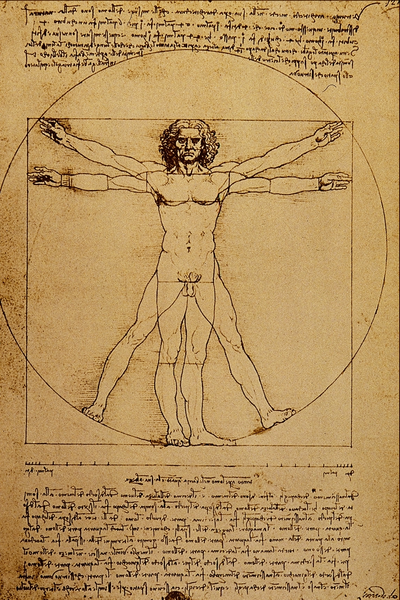
\includegraphics[scale=0.35]{img/vitruvian-man.png}
 \captionsetup{labelformat=empty}
 \caption{达$\cdot$芬奇,维特鲁威人,1490}
\end{figure}
%\end{wrapfigure}

\section{什么是对称}
对称究竟是什么?我们怎样精确地描述、甚至度量对称?让我们从最简单的左右双侧对称开始,理解什么是对称。观察《维特鲁威人》的上半部分,如果沿着中线为轴翻转,我们会得到同样的图形。将左右双侧对称的平面图形放到笛卡尔坐标平面上,让对称轴落在纵轴上,对称图形上的任何一点如果将横坐标翻转$x \mapsto -x$,则变化得到的图形和之前的叠合。而不对称的图形翻转后不会叠合。概括起来就是:

\[
f(x) = f(-x)
\]

进一步,如果把左右对称的图形抽象成一个线段,其端点为1、2,则交换端点为2、1图形仍然叠合,如图\ref{fig:reflection}所示。我们把这样的变换$(1, 2) \mapsto (2, 1)$称为一个置换。

\begin{figure}[htbp]
  \centering
  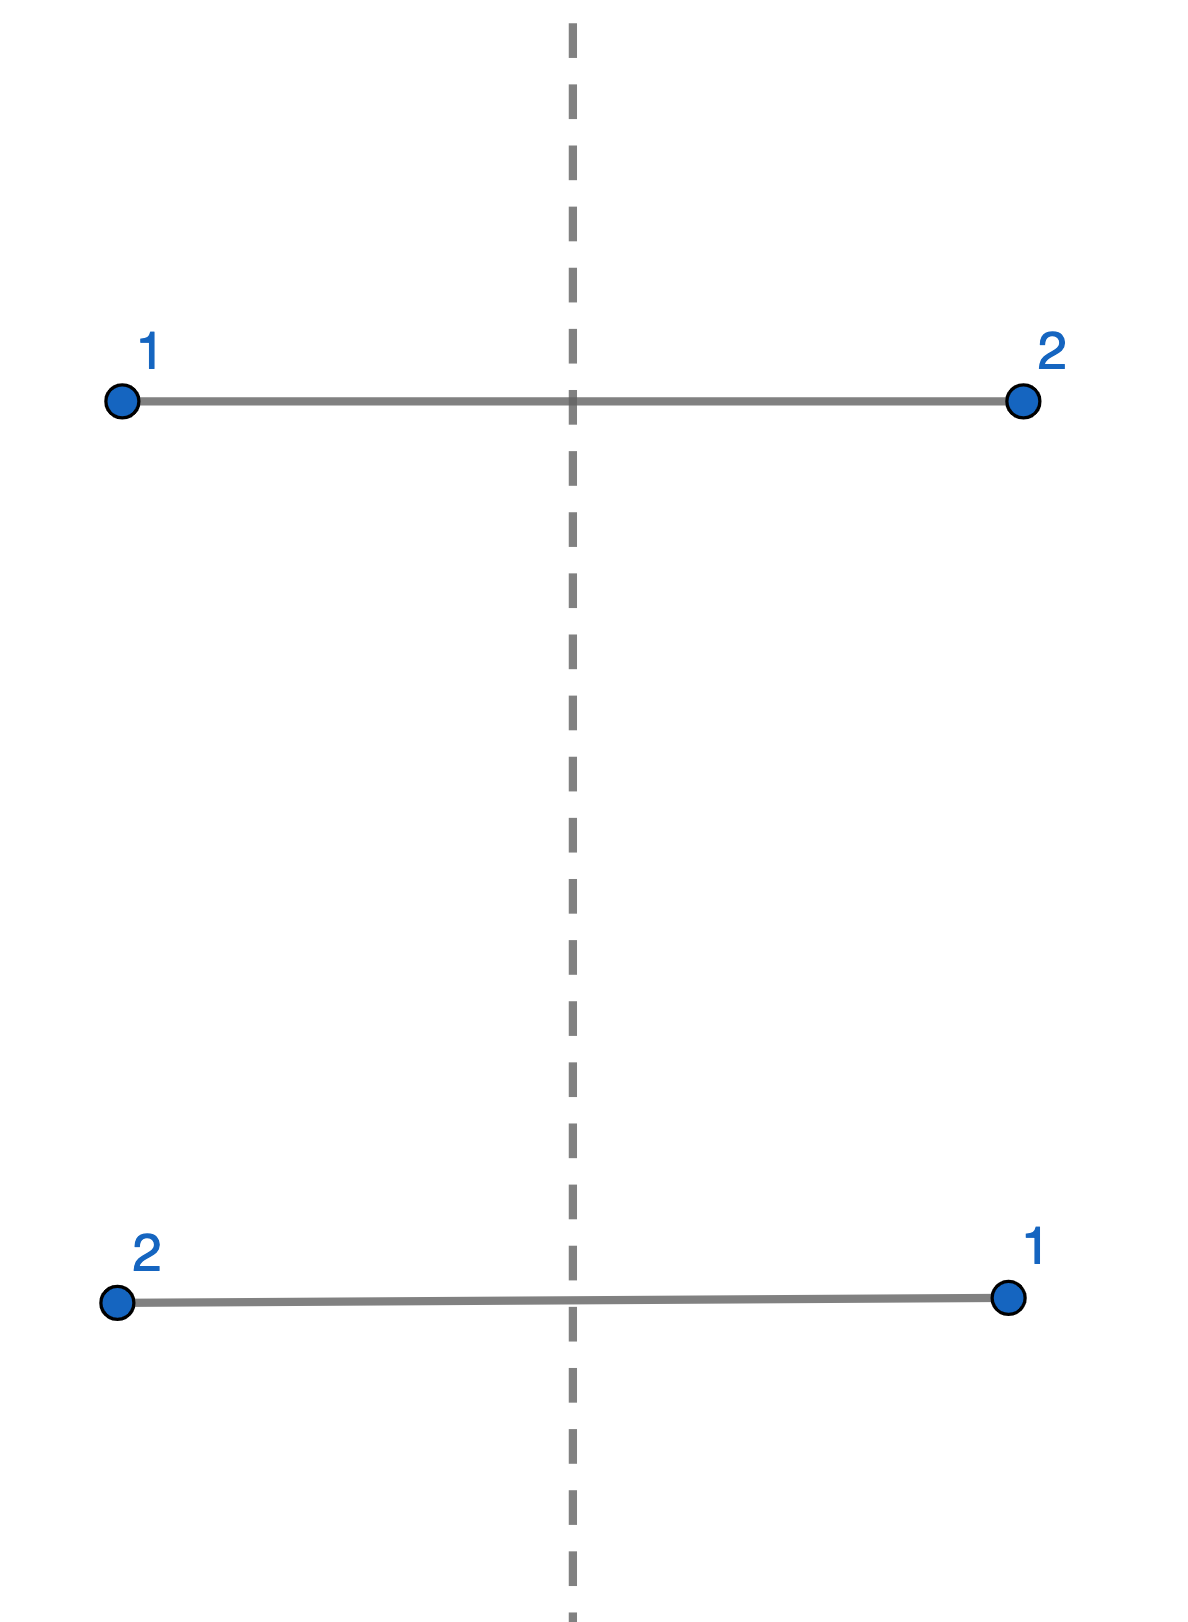
\includegraphics[scale=0.8]{img/reflection.png}
  \caption{左右双侧对称}
  \label{fig:reflection}
\end{figure}

对于两个元素的集合$\{a, b\}$,集合元素可以是任何东西,线段的两个端点,两对坐标,两个人,两段计算机程序等等。记第一个元素为1,第二个元素为2。存在两种置换:$(1, 2) \mapsto (2, 1)$和$(1, 2) \mapsto (1, 2)$。称第一种置换为“交换”,记为$s$,第二种置换为“恒等”,记为$e$。数学上常常采用下面的记法来表示置换:

\[ s = \begin{pmatrix}
1 & 2 \\
2 & 1 \\
\end{pmatrix}
,\
e = \begin{pmatrix}
1 & 2 \\
1 & 2 \\
\end{pmatrix}
\]

以置换$s$为例,它表示把第一行中的两个元素$1\ 2$,重新排列成第二行中的两个元素$2\ 1$。置换可以组合起来进行多次。$s \cdot s$表示连续交换两次:$(1, 2)  \arrowto{s} (2, 1) \arrowto{s} (1, 2)$。这样做的效果等于复原,或者说等同于恒等置换,即:$s \cdot s = e$。我们也可以说$s$相当于自己的“逆”置换:$s^{-1} = s$。我们把先执行一种置换,再执行另一种置换称为“组合”,用符号“$\cdot$”表示。对于$s$、$e$这两种置换,共存在4种组合:(1) $s \cdot e = s$、(2)  $e \cdot s = s$、(3) $s \cdot s = e$、(4) $e \cdot e = e$,可以用下面的“乘法表”形式加以总结:

\btab{c|cc}
$\cdot$  & s & e \\
\hline
s & e & s \\
e & s & e \\
\etab

这样的表格称为“凯莱”表,是英国数学家亚瑟$\cdot$凯莱提出的。点号可以省略,这样两个置换$\tau$、$\mu$的组合可以简记为$\tau\mu$。我们将上述置换的集合$\{s, e\}$及其元素之间的组合关系统称为$S_2$。它完整地描述了左右双侧对称。对于任何双侧对称的事物$a$,我们有$s(a) = a$。比如平面直角坐标$A = (-1, 0), B = (1, 0), C = (2, 0)$,因为$s(AB) = AB$,所以线段$AB$是左右对称的。而$s(AC)  \neq AC$,所以线段$AC$不是左右对称的。

把具有两个端点的线段扩展到三个端点的三角形,会有什么样的对称呢?记三个端点为1、2、3,我们发现一共存在6种置换,分别把端点置换为:$(2, 1, 3)$、$(3, 2, 1)$、$(1, 3, 2)$、$(2, 3, 1)$、$(3, 1, 2)$、$(1, 2, 3)$。其中最后一种是恒等置换,记为$e$。以图\ref{fig:triangles}中间的的三角形为例,第一种交换1、2而固定3不变,相当于以中线做镜像翻转,记为$s$。第四种置换相当于把三角形顺时针旋转,记为$r$,而第五种相当于逆时针旋转,记为$r^{-1}$。我们将这6种置换及其间的组合关系称作$S_3$。显然图中的三个三角形的对称性是不同的。最左边的三角形只在恒等置换$e$下不变。它的对称性最低;中间的等腰三角形在置换$s$和$e$下不变,对称性比左边的高;右边的正三角形在6种置换下都不变,具有最高的对称性(三条镜像对称轴、绕中心旋转$\pm\dfrac{2\pi}{3}$)。我们看到$S_3$可以度量三角形的对称性。

\begin{figure}[htbp]
  \centering
  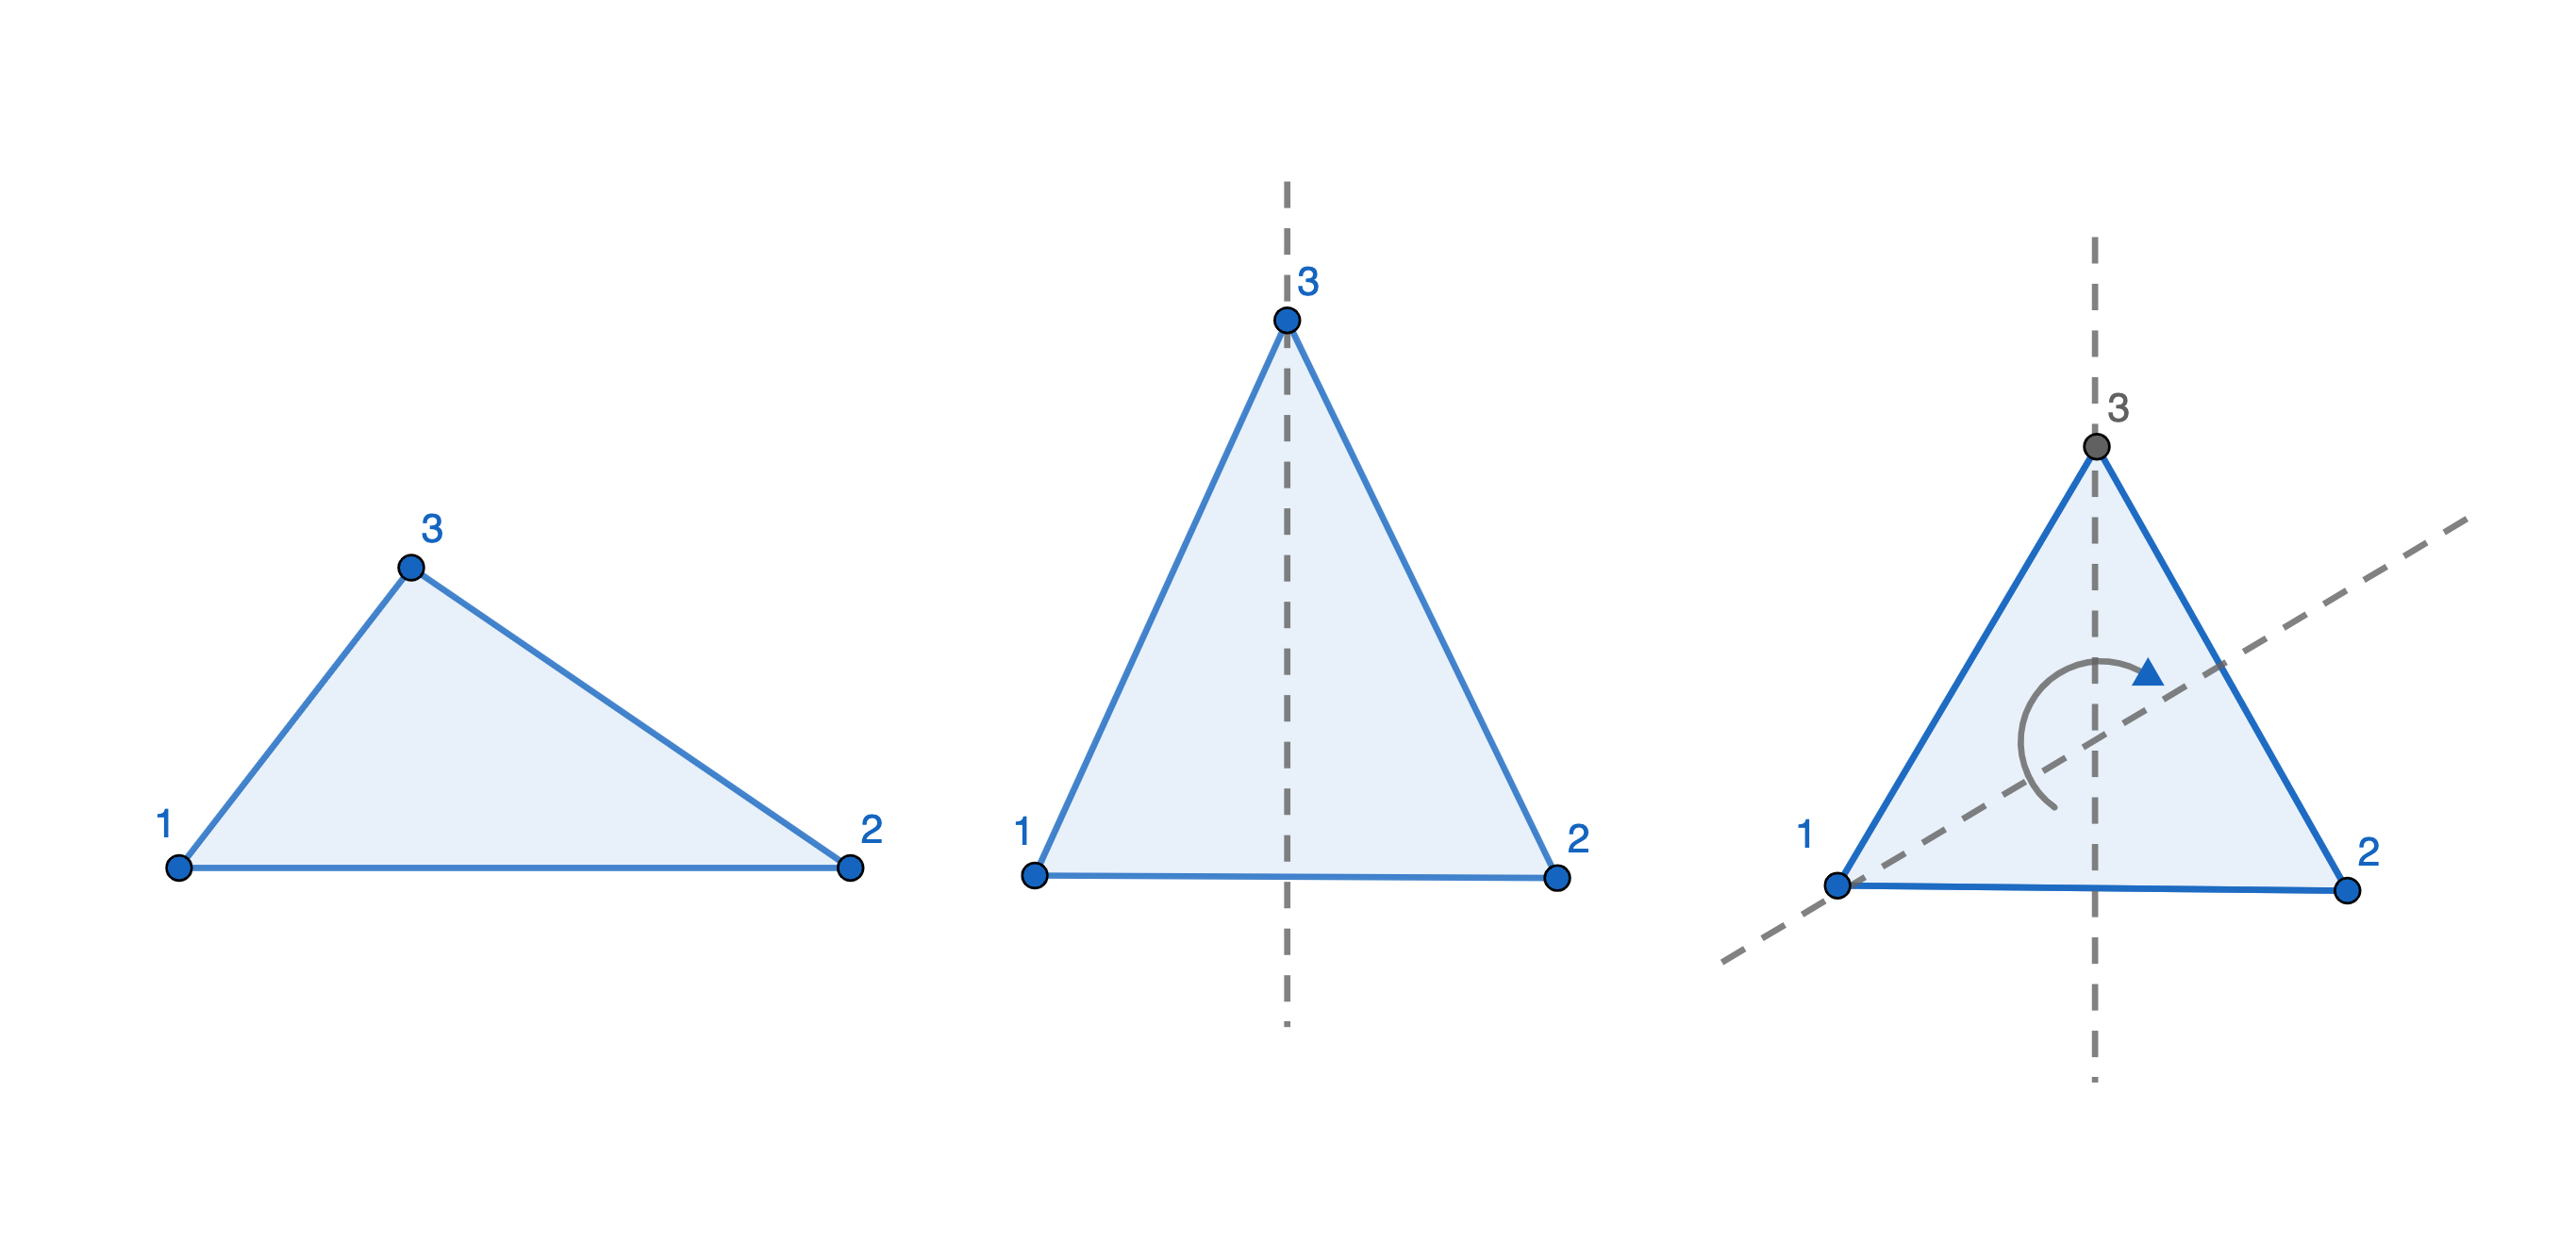
\includegraphics[scale=0.6]{img/triangles.png}
  \caption{三角形的对称}
  \label{fig:triangles}
\end{figure}

这6种置换是可以相互组合的。例如先逆时针旋转$r^{-1}$,再镜像翻转$s$,就得到了第二种置换,即:$(2, 1, 3) (3, 1, 2) = (3, 2, 1)$。而逆时针旋转可以通过两次顺时针旋转来得到,即:$r^{-1} = rr$。这6种置换,可以只用$s$、$r$、$e$来表示。下面给出了$S_6$的的凯莱表:

\btab{c|cccccc}
 & $s$ & $sr^{-1}$ & $sr$ & $r$ & $r^{-1}$ & $e$ \\
\hline
$s$ & $e$ & $r^{-1}$ & $r$ & $sr$ & $sr^{-1}$ & $s$ \\
$sr^{-1}$ & $r$ & $e$ & $r^{-1}$ & $s$ & $sr$ & $sr^{-1}$ \\
$sr$ & $r^{-1}$ & $r$ & $e$ & $sr^{-1}$ & $s$ & $sr$ \\
$r$ & $sr$ & $s$ & $sr^{-1}$ & $r^{-1}$ & $e$ & $r$ \\
$r^{-1}$ & $sr^{-1}$ & $sr$ & $s$ & $e$ & $r$ & $r^{-1}$\\
$e$ & $s$ & $sr^{-1}$ & $sr$ & $r$ & $r^{-1}$ & $e$ \\
\etab

$S_2$、$S_3$不仅可以反应线段、三角形的空间对称性,还可以刻画抽象事物的对称性。我们考虑方程$x^2 + px + q = 0$的两个解$x_1, x_2$,根据初中数学中的韦达定理,我们有:

\be
\begin{cases}
x_1 + x_2 = -p \\
x_1 x_2 = q
\end{cases}
\ee

把$S_2$应用上去,我们发现用$s$交换两个根,方程和韦达定理都仍然成立。加上恒等变换$e$,我们发现$S_2$可以描述一元二次方程的对称性。韦达进一步发现,对于三元方程$x^3 + rx^2 + px + q = 0$也有类似的定理:

\be
\begin{cases}
x_1 + x_2 + x_3 = -r \\
x_1 x_2 + x_2 x_3 + x_3 x_1 = p \\
x_1 x_2 x_3 = -q
\end{cases}
\ee

其中$x_1$、$x_2$、$x_3$是方程的三个根。不难发现在$S_3$中的6种置换下,方程和韦达定理也都成立。$S_3$描述了一元三次方程的对称性。在历史上,正是这种发现孕育出了一个全新的数学分枝。数学家们发展出了群来定义、描述、度量对称。并且发现方程可解性的问题,究其本质是方程根的对称性问题、因而一举用群的方法突破了几百年来的未解之谜,并且回答了早在古希腊时就困扰着人们的三大作图难题。本章我们以对称为线索介绍一些抽象的代数结构,它们不仅仅是对数的抽象,而且是对事物的概念、性质、关系的抽象,是很多伟大的思想和心智的结晶。有些部分难度较大,挑战我们抽象思维的极限。因此我在其中穿插介绍了前辈数学家们是如何披荆斩棘、取得突破的故事。即使读完这一章没有能领会抽象的知识,我也希望这些令人感慨的故事能不断激励我们前行。

%% 在发展抽象的方法和工具时,必须时刻关注一个问题:“某一种抽象的适用范围有多大?什么情况下这一抽象会失效?”如果忽略了这一点,就会产生令人啼笑皆非的结果。比如人们总结抽象出了无穷几何级数的累加公式:$1 + x + x^2 + x^3 + ... = 1/(1-x)$。并用它成功解决了芝诺悖论\footnote{古希腊哲学家芝诺提出了四个著名的悖论,这里是指阿基里斯与乌龟悖论。阿基里斯是古希腊著名的英雄。芝诺假设阿基里斯追赶前面的乌龟,当他跑到乌龟出发的位置时,乌龟已经向前移动了一小段距离。阿基里斯必须继续跑到乌龟的新位置,但是此时乌龟又向前移动了。重复这一过程,芝诺认为阿基里斯永远赶不上乌龟。本书在第五章详细解释芝诺悖论。}。但是17世纪的数学家们把-1代入这个公式得到了$1 - 1 + 1 - 1 + ... = 1/2$这样的结果。这时有人提出了不同的意见:$S = (1 - 1) + (1 - 1) + ... = 0$;还有人认为:$S = 1 + (-1 + 1) + (-1 + 1) + ... = 1$。有人赞同1/2的结果,因为$S = 1 - (1 - 1 + 1 - 1 + ...) = 1 -S$,解方程得$S = 1/2$。意大利数学教授格兰迪(1671 - 1742)还发现了更令人吃惊的结论。通过无穷级数:

%% \[
%% \def\arraystretch{2.2}
%% \begin{array}{l}
%% \dfrac{1}{1 + x + x^2} = 1 - x + x^3 - x^4 + x^6 - x^7 + ... \\[2ex]
%% \dfrac{1}{1 + x + x^2 + x^3} = 1 - x + x^4 - x^5 + x^8 - x^9 + ... \\
%% ...
%% \end{array}
%% \]

%% 令$x = 1$,格兰迪发现无穷级数$1 - 1 + 1 - 1 + 1 - 1 + ...$的和可以等于1/3, 1/4, ...就连大数学家莱布尼茨也主张,它的和可能是0或者1,而且概率相等,所以其“真”值应该是它们的平均值1/2。格兰迪还做出了另一个“奇妙”的解释:父亲留给两个儿子一块宝石,由兄弟二人轮流保存,每人一年。于是,交给对方保存的时候,可以说所有权是0,自己保存的时候,可以说所有权是1,而平均而言,每人的所有权为1/2\cite{HanXueTao16}。这些奇怪的问题,要等到法国数学家柯西引入无穷级数收敛性后才得以解决。

\begin{Exercise}
\Question{编程判断一棵二叉树是否是左右对称的。}
\end{Exercise}

\section{群}

\begin{figure}[htbp]
%\begin{wrapfigure}{R}{0.4\textwidth}
 \centering
 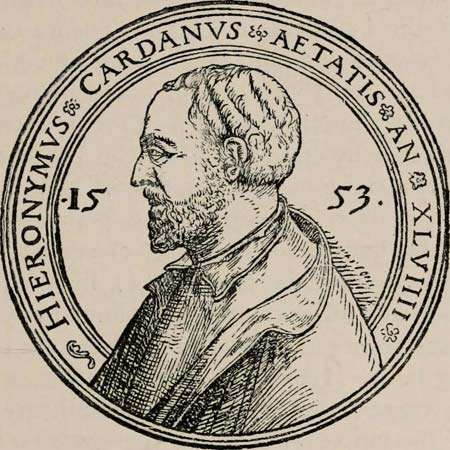
\includegraphics[scale=0.3]{img/Cardano.jpg}
 \captionsetup{labelformat=empty}
 \caption{卡尔丹(Gerolamo Cardano, 1501-1576)}
 \label{fig:Cardano}
%\end{wrapfigure}
\end{figure}

\index{卡尔丹(Gerolamo Cardano)}
\index{高斯}
\index{代数基本定理}
提到群论(Group theory),就不得不提人类解方程的历史。方程是我们祖先发展出的一个强大工具。人们从古埃及的纸草书和古巴比伦的泥板书中发现,这些古代文明已经掌握了一元一次和二次方程的解法。但是一般三次方程的解法却一直没有进展。到了16世纪,经过意大利数学家们的努力,终于得到了一般三次方程和四次方程的根式解。最终卡尔丹在他的著作《大术》中总结人类历史上这千余年的结果。这些进展并不仅仅是未知数次数的提升,我们对数还有了全新的认识。早期二次方程的负根都被舍弃了,人们认为负数没有意义。不仅如此,人们认为方程的系数也必须是正数,在我们今天看来普通的方程$x^2 - 7x + 8 = 0$,必须用$x^2 + 8 = 7x$的形式来处理。在《大术》中,卡尔丹列出了20种不同类型的四次方程,他说还有67种其它类型的四次方程没有给出,原因仅仅是因为四次方程各项的系数可以为负数和零\cite{HanXueTao2012}。直到法国数学家韦达才将方程的形式统一。在解方程时,负数的根式一直被认为是无意义的。但是卡尔丹在解三次方程,例如$x^3 = 15x +4$时,他的公式给出了$\sqrt[3]{2 + \sqrt{-121}} + \sqrt[3]{2 - \sqrt{-121}}$这样的中间结果。而我们知道这一方程有三个实根4, $-2 \pm \sqrt{3}$。这些问题拓展了我们对虚数的认识,并最终在高斯的手中,建立了代数基本定理\footnote{高斯一生多次证明了代数基本定理。1799年,22岁的高斯在其博士论文中证明了实系数一元$n$次方程至少有一个复数根。由此推出$n$次方程有且仅有$n$个复根(重根按重数计算)。高斯又在1815和1816年给出了另外两个证明。1849年,在庆祝取得博士学位50周年的纪念会上,高斯又发表了第四个证明,并把系数也推广到了复数。}。

\begin{figure}[htbp]
%\begin{wrapfigure}{R}{0.3\textwidth}
 \centering
 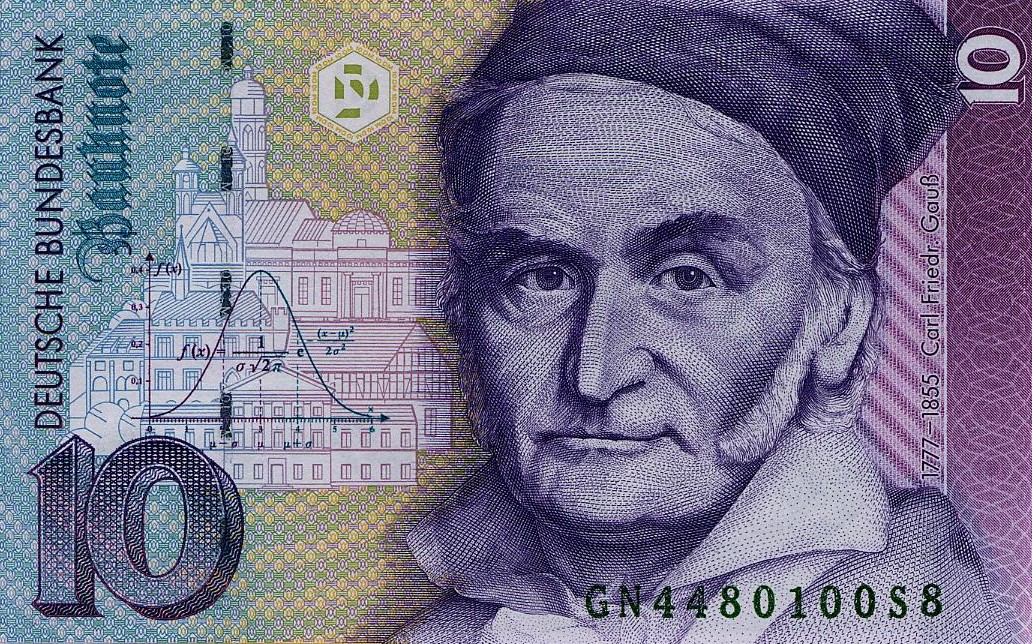
\includegraphics[scale=0.25]{img/Gaus.jpg}
 \captionsetup{labelformat=empty}
 \caption{十马克上的高斯像。高斯(1777-1855)}
 \label{fig:Gauss}
%\end{wrapfigure}
\end{figure}

然而接下来在寻找五次及以上方程的根式解时,人们遇到了前所未有的困难。经历了近300年的苦苦寻找,终于在19世纪迎来了出乎意料的结果。1799年,意大利数学家鲁菲尼转而试图证明一般的五次方程没有根式解。遗憾的是他的方法存在漏洞,在当时没有得到足够重视。1824年,挪威的青年数学家阿贝尔终于独立给出了完整的证明。这一结论现在称为“阿贝尔-鲁菲尼定理”。然而,这一定理只是说一般的五次方程没有根式解,我们知道$x^5-1=0$是有根式解的。什么情况下一个多项式方程有根式解呢?法国的天才少年伽罗瓦用他独创的想法,彻底解决了这个问题\cite{Wiki-Galois-theory}。

\begin{figure}[htbp]
%\begin{wrapfigure}{L}{0.4\textwidth}
 \centering
 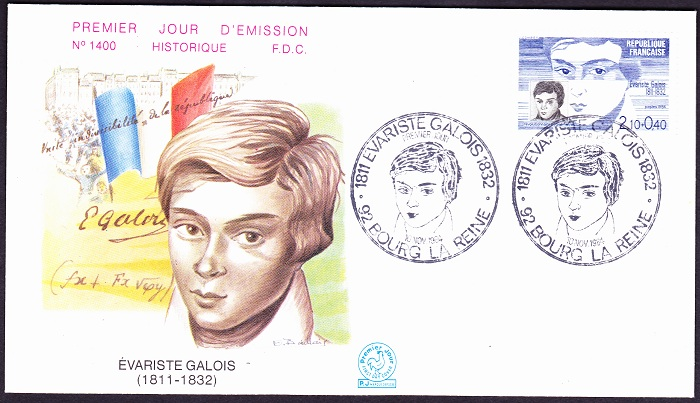
\includegraphics[scale=0.4]{img/galois.jpg}
 \captionsetup{labelformat=empty}
 \caption{伽罗瓦(1811 - 1832)}
 \label{fig:Galois}
%\end{wrapfigure}
\end{figure}

\index{伽罗瓦(Galois)}
伽罗瓦短短的20年人生上演了一幕悲剧,然而他身后却开辟了抽象代数这一数学分支。1811年10月25日,伽罗瓦生于巴黎。他的母亲精通拉丁文和古典文学。在12岁前他一直由母亲进行启蒙教育。1823年,伽罗瓦进入巴黎的“路易大帝”中学读书。到了14岁,他开始如饥似渴地学习起数学来。他找来一本勒让德改编的《几何原本》,像读小说一样迅速地掌握了。15岁时,他已经四处寻找拉格朗日的原著来读了。拉格朗日在1770年写的一遍关于方程的预解式的文章可能对伽罗瓦日后的工作产生了重要的影响。他的水平迅速超出了老师的能力范围。但是这位天才少年除了数学对其它学科都不感兴趣。

1828年6月,伽罗瓦参加了法国最富盛名的巴黎综合工科学校的入学考试。这所大学是法国大革命的产物,拿破仑对它倍加支持和保护。在数学口试中,他认为某些结论很显然,于是不进行解释,结果伽罗瓦落榜了。1829年4月,伽罗瓦发表了第一篇关于连分数的论文。在这一时期,伽罗瓦在多项式方程上取得了重大的发现。他向法国科学院提交了两篇论文。但由于种种原因,论文没有通过\footnote{有说法认为由于审稿人柯西的疏忽这些论文丢失了。柯西实际上推荐了伽罗瓦的论文,但认为不够清晰,不能发表。人们普遍认为柯西认识到了伽罗瓦工作的重要性, 他只是建议将这两篇论文合并成一个, 以便能够角逐科学院的数学大奖。柯西是当时著名的数学家, 虽然与伽罗瓦的政治观点不同, 但仍认为伽罗瓦能够赢得大奖。\cite{Wiki-Galois}}。打击接踵而至,1829年7月28日,伽罗瓦的镇长父亲因屈服于政敌的恶意攻击自杀身亡\footnote{他与村里的牧师发生了激烈的政治争执后自杀\cite{Wiki-Galois}。}。8月3日,伽罗瓦在服丧期间第二次也是最后一次参加他渴望的巴黎综合工科学校的入学考试。父亲的去世多少对他有影响。在口试阶段,主考官问他一个对数级数的结果是怎样得来的。伽罗瓦跳过了中间步骤说结果很显然,这令考官很恼火,结果他又没有通过。据说伽罗瓦愤怒地把黑板擦投到了主考官的脸上。最后他不得不参加高等师范学校的考试。当时的数学主考官写道:“该生在表达自己的想法时有时很晦涩, 但他很聪明, 表现出非凡的研究精神。”

1830年,在柯西的建议下,伽罗瓦把论文提交给了科学院秘书傅里叶以角逐法兰西科学院的数学大奖。傅里叶把论文带回家中,但未及审阅就去世了。结果伽罗瓦的论文丢失,科学院于1830年6月把大奖授予了阿贝尔\footnote{年轻的阿贝尔已于1829年4月6日在贫病交加中去世了,年仅26岁。他是椭圆函数领域的开拓者,阿贝尔函数的发现者。第一个证明了五次方程无根式解。他还研究了更广的一类代数方程,后人发现这是具有交换的伽罗瓦群的方程。为了纪念他,后人称交换群为阿贝尔群。}和雅可比\cite{HanXueTao2009}。

\begin{figure}[htbp]
%\begin{wrapfigure}{L}{0.4\textwidth}
 \centering
 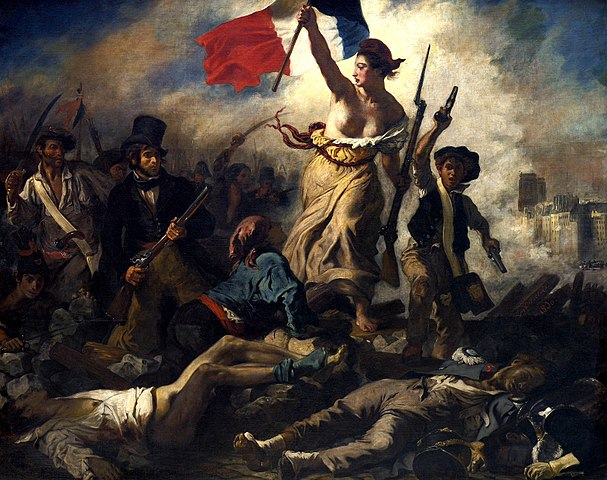
\includegraphics[scale=0.4]{img/lltp.jpg}
 \captionsetup{labelformat=empty}
 \caption{欧仁·德拉克罗瓦《自由引导人民》1830,巴黎卢浮宫收藏}
 \label{fig:Liberty-Leading-the-People}
%\end{wrapfigure}
\end{figure}

伽罗瓦生活在政治动荡时期。1830年法国爆发了七月革命\footnote{拿破仑在滑铁卢惨败后,波旁王朝复辟。查理十世清洗了军队中曾为拿破仑效力的军人,引起了人民的不满。并在政治经济、文化宗教和外交中不断失政。查理十世在7月25日颁布圣卢克法令,宣布限制出版自由,解散议会,修改选举法。直接引发了人民的武装起义,通过革命推翻波旁王朝,拥戴路易$\cdot$菲利普登上王位,建立七月王朝。}。因为激进的革命立场,伽罗瓦被学校开除了。他参加了国民自卫军,一边革命一边进行数学研究。1830年12月,国民自卫军被解散,伽罗瓦曾经一度被捕, 但于1831年6月15日被判无罪释放。1831年7月14日法国国庆,伽罗瓦穿上了被解散的国民自卫军军装,拿着上膛的长短枪支上街游行。他因此再次被判入狱6个月。在此之前的1831年1月17日,在数学家泊松的建议下,伽罗瓦又一次将他的方程理论提交给法国科学院。结果泊松也没有能理解伽罗瓦的全新思想。7月4日,负责论文审阅的泊松声称:“论证既不够清晰,又不够详尽,使我们无法判断其严格性\footnote{但是,泊松在论文审阅的报告结尾处鼓励道:“我们建议作者应公布他的全部工作, 以便形成一个明确的意见。”}。”由于伽罗瓦在7月14日被捕,直到10月份他在狱中才收到论文拒绝发表的消息。心高气傲的伽罗瓦反应强烈,他放弃了正规学术途径,转而求助于他的朋友奥古斯特$\cdot$谢瓦利耶(Auguste Chevalier)私人发表论文。伽罗瓦注意到了泊松的建议,他在狱中开始整理数学手稿,并不断完善他的思想,直到1832年4月29日出狱。

出狱后不久,伽罗瓦因为爱情卷入了一场无谓的决斗。5月29日决斗前夕,深信自己将在决斗中死去的伽罗瓦写了三封信。最长的第三封信是写给朋友谢瓦利耶的,短短7页中包含了一份数学思想纲要和三份手稿。这份纲要十分简洁,但内容却极为丰富。只有在后来人把它展开的时候,其重要性才渐渐为人所理解。而且预见了很久以后的发现,证明了伽罗瓦深刻的洞察力。数学家赫尔曼$\cdot$外尔认为:“从创新程度与思想深度来看,这封信有可能是有史以来份量最重的一篇文字。”信中还有一些后人读来无比惋惜的文字:“这些题目并非我已研究的全部……我没有时间,在我有兴趣的领域里,我已宣布但尚未证明,从而使人怀疑的定理确实是太多了。”其中最令人难忘的,也是最悲伤的话语是:“我没有时间了。”在信的末尾,他要求他的朋友“请求雅可比或者高斯就这些定理的重要性(而不是正确与否)公开发表他们的看法。我希望将来有人能意识到它们是有益的。”

\begin{figure}[htbp]
%\begin{wrapfigure}{L}{0.4\textwidth}
 \centering
 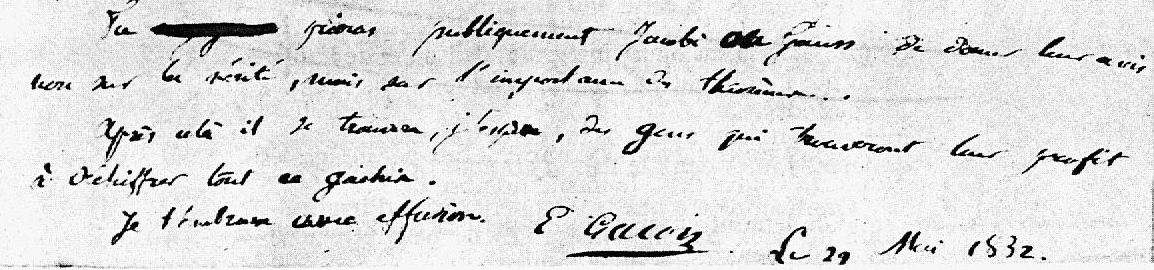
\includegraphics[scale=0.3]{img/GalSign.png}
 \captionsetup{labelformat=empty}
 \caption{伽罗瓦在决斗前夜最后一封信上的签名``E. Galois, le 29 mai 1832''}
 \label{fig:GalSign}
%\end{wrapfigure}
\end{figure}

1832年5月30日早晨,伽罗瓦在决斗受了重伤,一个路过的农民发现了他。9点半,他被送到医院。他拒绝了牧师的祈祷,对赶来的弟弟说:“阿尔弗莱德,不要哭。在20岁就死去,需要我全部的勇气。”次日上午10时,伽罗瓦停止了呼吸。关于决斗的原因,有各种不同的说法。人们不知道这是一个悲惨的爱情事件还是政治谋杀。无论是哪一种,一位世界上最杰出的数学家在他20岁时被杀死了,他研究数学只有5年,而其全部数学成果仅有67页。

谢瓦利耶和伽罗瓦的弟弟按照他的遗愿将其工作发表在《百科评论》上,但没有对当时的数学发展产生影响。也许是因为它太晦涩简略了\footnote{同样的教训也发生在阿贝尔身上,1824年他自费印刷发表关于一般五次方程没有根式解的论文。为了省钱,他拼命把论文压缩到6页纸内。结果由于太过简略晦涩,在阿贝尔生前,几乎没有人注意到这一成果。}。直到14年后的1846年,法国数学家刘维尔领悟到伽罗瓦思想的价值,将这些论文编辑发表在极有影响的《纯粹与应用数学》杂志上。在对论文的介绍中,刘维尔对伽罗瓦的悲剧进行了反思:“过分地追求简洁是导致这一缺憾的原因。人们处理像纯粹代数这样抽象和神秘的事物时,应该首先尽力避免这样做。事实上,当你试图引导读者远离习以为常的思路进入较为困惑的领域时,清晰性是绝对必须的……但是现在一切都改变了,伽罗瓦再也回不来了!我们不要再过分地做无用地批评,让我们把缺憾抛开,找一找有价值的东西……我的热心得到了好报,在填补了一些细小的缺陷后,我看出伽罗瓦用来证明这个定理的方法是美妙和完全正确的,在那个瞬间,我体验到了一种强烈的愉悦。”1870年法国数学家约当根据伽罗瓦的思想,撰写了《置换与代数方程》一书\footnote{伽罗瓦理论无疑是相当艰深,并且超越于他的时代的。刘维尔在1846年发表整理伽罗瓦的论文时,在注释中完全忽略了群的核心思想。塞雷参加了刘维尔的讲座后,在他的书中开始介绍伽罗瓦理论。约当是塞雷的学生。伽罗瓦理论在非法语国家被接受得更晚。英国要到一个世纪后,而德国直到哥廷根时代,才由戴德金在课上讲授。},伽罗瓦的最主要成就是提出了“群”的概念,并用群论彻底解决了根式求解代数方程的问题,而由此发展出了一整套关于群和域的理论。为了纪念他,人们称之为伽罗瓦理论。正是这套理论创立了抽象代数学,标志着数学发展现代阶段的开始。有人评论道:“伽罗瓦一心想要参加的是政治革命,然而实际上所引发的却是数学革命。\cite{StepanovRose15}”

\subsection{群的定义}
\index{群的定义}

我们前面提到可以描述双侧对称性的$S_2$和三角形对称性的$S_3$其实是群这个大家族中的两个成员。总结它们的共同点,我们可以得到群的定义:

\begin{definition}群是一个集合$G$与其上定义的某种二元运算“$\cdot$”。它遵循四条公理:
\begin{enumerate}
\item 封闭性公理:对任何$a, b \in G$,运算结果$a \cdot b \in G$;
\item 结合性公理:对任何$a, b, c$,有$(a \cdot b) \cdot c = a \cdot (b \cdot c)$;
\item 单位元公理:$G$中存在一个元素$e$,使得对任何$a \cdot e = e \cdot a = a$;
\item 消去公理:对任何$a \in G$,都存在一个逆元$a^{-1}$使得$a \cdot a^{-1} = a^{-1} \cdot a = e$。
\end{enumerate}
\end{definition}

方便起见,我们有时称二元运算为“乘法”,并且省略掉点,将$a \cdot b$写成$ab$。我们称$e$为单位元。一个群的元素个数可以有限也可以无限,分别称为有限群和无限群。元素的个数叫做这个群的阶。

群的“乘法”运算并不一定像数的乘法运算那样满足交换律。例如所有元素为实数的可逆矩阵与矩阵乘法组成一个群。但矩阵乘法的顺序是不可交换。如果群中的二元运算满足交换律,则称为交换群。为了纪念挪威数学家阿贝尔,人们称交换群为阿贝尔群。为了帮助理解这一抽象定义,我们来看一些具体的群的例子。

\begin{enumerate}
\item 整数加法群:群元素是全体整数,二元运算是加法。简称为整数加群;
\item 所有整数除以5的余数构成的集合,也就是$\{0, 1, 2, 3, 4\}$。二元运算是相加后再除以5取余数。例如$3 + 4 = 7 \bmod 5 = 2$。这样构成的群称为整数模5加法群,记为$Z_5$。通过取余数对整数进行分类叫做模$n$剩余类\footnote{现代记法为$\pmb{Z}/5\pmb{Z}$};
\item 转动魔方所形成的群:群元素是各种魔方转动的方式\footnote{魔方的旋转方式共有18种。可以沿着正面、反面、顶面、底面、左面、右面旋转,分别用字母$F$、$B$、$T$、$D$、$L$、$R$代表,每面可以旋转90度、180度、-90度。例如左面旋转90度、180度、-90度分别可以记为:$L$、$L^2$、$L'$\cite{Wiki-Rubik-Cube-group}。再加上恒等变换,一共19个元素。},二元运算是先进行某种转动后再进行另一种转动。这种运算常被称作转动的合成;

\begin{figure}[htbp]
%\begin{wrapfigure}{L}{0.4\textwidth}
 \centering
 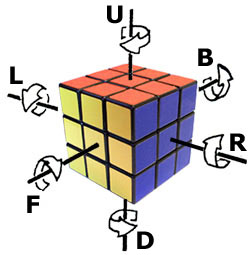
\includegraphics[scale=0.6]{img/Rubik_cube_notation.jpg}
 %\captionsetup{labelformat=empty}
 \caption{魔方六个面共有18种转动方式,再加上恒等变换。这些转动方式在合成下构成一个群。}
 \label{fig:Rubik-cube-notation}
%\end{wrapfigure}
\end{figure}

魔方的初始状态是6个面都是均一颜色。我们可以让一个小孩子通过一系列的随意转动打乱魔方。所谓还原魔方,是要求玩魔方的人,开动脑筋,通过一系列的转动恢复成6个面均一颜色的状态。如果我们把打乱过程的转动记录下来:$\{t_0, t_1, ..., t_m\}$,把还原的过程也记录下来:$\{r_0, r_1, ..., r_n\}$。打乱再还原的过程相当于:

\[
  (r_n \cdot r_{n-1} ... \cdot r_0) \cdot (t_m \cdot t_{m-1} ... \cdot t_0) = e
\]

显然,一种还原方法是把打乱过程中的每一步都反向转动,即:$r_i = t_{m-i}^{-1}$,也就是$r_i \cdot t_{m-i} = e$。这样上式一定成立。但实际中,魔方高手往往通过一定的方法,也就是所谓魔方公式,进行还原。这样尽管上式成立,但是并不是每个$r_i$都是某个$t_{m-i}$的逆元,甚至打乱和还原的步数也通常不相同。

\item 平面绕某点的所有旋转构成一个群。群元素是所有的旋转角度,二元运算是先旋转某一角度,然后再旋转另一角度。单位元是零度。

所谓平面图形的“旋转对称”,是指图形上的所有点旋转一定角度后,和原来的图形重合。例如雪花绕中心旋转$60\degree$、$120\degree$、$180\degree$、$240\degree$、$300\degree$、$360\degree$后仍然和自己重合。当然。例子中的旋转群无法描述雪花的对称。这个群揭示了这样的事实。如果两个角度的变换$r_{\alpha} \cdot r_{\beta} = e$,那么这两个角度要么相反$\alpha = -\beta$,要们它们相加是$360\degree$的整数倍。在这个旋转群下,唯一对称的一种图形是同心圆。我们将在后面小节给出雪花的对称群。

\end{enumerate}

而下面这些不是群:

\begin{enumerate}
\item 所有不等于零的整数和乘法不构成群,我们不能规定单位元为1,因为3没有逆元(1/3不是整数);
\item 同理,模5的余数集合$\{0, 1, 2, 3, 4\}$和模5的乘法不构成一个群,但如果把5的整倍数去掉,则集合$\{1, 2, 3, 4\}$和模5的乘法构成一个群。可以从下面的凯莱“乘法表”看出来:

\btab{c|cccc}
    & 1 & 2 & 3 & 4 \\
  \hline
  1 & \textbf{1} & 2 & 3 & 4 \\
  2 & 2 & 4 & \textbf{1} & 3 \\
  3 & 3 & \textbf{1} & 4 & 2 \\
  4 & 4 & 3 & 2 & \textbf{1}
\etab

因此,单位元是1,它的逆元是其本身;2和3互为逆元,4的逆元还是4;
\item 虽然模5的非零余数在模乘法下构成一个群,但是模4的非零余数在模乘下却不构成群。观察模4的凯莱乘法表:

\btab{c|cccc}
    & 1 & 2 & 3 \\
  \hline
  1 & 1 & 2 & 3 \\
  2 & 2 & \textbf{0} & 2 \\
  3 & 3 & 2 & 1 \\
\etab

注意到$(2 \times 2) \bmod 4 = 0$,不在集合$\{1, 2, 3\}$中。只有和$n$互素的余数集合,在模$n$乘法下才能构成群,这种群称为整数模$n$乘法群。自然,如果$p$是素数,则$\{1, 2, ..., p-1\}$构成模$p$乘法群。
\item 全体有理数在乘法下不构成一个群。尽管任何形如$p/q$的有理数($p, q$都不为0)都有逆元$q/p$,但是0没有逆元。所有非零有理数在乘法下才构成一个群。
\end{enumerate}

\begin{Exercise}
\Question{全体偶数在加法下是否构成一个群?}
\Question{能否找到一个整数的子集,使得它在整数乘法下构成一个群?}
\Question{所有正实数在乘法下是否构成一个群?}
\Question{整数在减法下是否构成一个群?}
\Question{举一个只有两个元素的群的例子。}
\Question{魔方群的单位元是什么?$F$的逆元是什么?}
\end{Exercise}

\subsection{幺半群与半群}
群的限制条件比较严格,从上一节的反例中,我们看到有一些常用的代数结构无法满足群的全部条件。有时我们并不需要一定能够取逆元,如果放宽条件,就可以得到幺半群(monoid)这种结构。

\index{幺半群(monoid)}
\begin{definition}
\textbf{幺半群}是一个集合$S$和其上定义的二元运算$\cdot$,它们遵循两条公理:
\begin{enumerate}
\item 结合性公理:$S$中和任何三个元素满足$(a \cdot b) \cdot c = a \cdot (b \cdot c)$;
\item 单位元公理:$S$中存在一个元素$e$,使得对任何$a \cdot e = e \cdot a = a$。
\end{enumerate}
\end{definition}

可以看到幺半群与群的定义类似,只是去掉了取逆运算的消去公理。上一节群的反例中有不少是幺半群,例如整数乘法构成幺半群,单位元是1。幺半群在编程中很常见。我们在下一章范畴论中还会再仔细介绍它。下面是一些幺半群的例子:

\begin{enumerate}
\item 给定字符集后,长度有限的字符串在拼接操作下构成幺半群。幺半群的元素是字符串,二元运算是拼接操作。单位元是空串。
\item 由字符串推广到列表(元素类型为A的列表记为:List A),在连接操作下构成幺半群。幺半群的元素是列表,二元运算是连接操作($\doubleplus$)。单位元是空列表nil。

为此,我们可以写出以下的程序,用幺半群来定义字符串和列表的代数结构。

\begin{lstlisting}
instance Monoid (List A) where
    e = nil
    (*) = (++)
\end{lstlisting}

这样针对字符串和列表的的“叠加”操作,完全可以将抽象程度提升到幺半群上来\footnote{我们将在下一章讲解范畴论时介绍如何实现这样的抽象叠加操作}。例如下面的“合并”操作定义对任何幺半群都有效:

\[
concat = foldr\ e\ (*)
\]

这样就可以用$concat$合并列表,如

$concat\ [[1], [2], [3], [1, 2], [1, 3], [2, 3], [1, 2, 3], [1, 3, 2]]$的结果是[1, 2, 3, 1, 2, 1, 3, 2, 3, 1, 2, 3, 1, 3, 2]。

\index{堆(heap)}
\index{斜堆(skew heap)}
\item 堆(heap)是编程中一种常见的数据结构,堆顶元素总是最小的堆称为最小堆(或小顶堆、小根堆)。有一种“斜堆”(skew heap)可以用上一章定义的二叉树来实现(\cite{LiuXinyu2017}第7.3节):

\begin{lstlisting}
data SHeap A = nil | node (SHeap A, A, SHeap A)
\end{lstlisting}

可以看出,除了名称,斜堆的定义和二叉树完全一样。非空堆的最小元素在树的根节点中。定义斜堆的“归并”(merge)运算如下:

\[
\begin{array}{rcl}
merge(nil, h) & = & h \\
merge(h, nil) & = & h \\
merge(h_1, h_2) & = &
  \begin{cases}
  k_1 < k_2 : & node(merge(r_1, h_2), k_1, l_1) \\
  \text{否则}: & node(merge(h_1, r_2), k_2, l_2)
  \end{cases}
\end{array}
\]

如果其中任一堆为空,则归并结果为另一个堆。非空情况下,$h_1$和$h_2$分别可以表示为 $node(l_1, k_1, r_1)$ 和 $node(l_2, k_2, r_2)$。我们比较根节点,选择较小的作为新的根。然后把含有较大元素的树合并到某一子树上。最后再把左右子树交换。若$k_1 < k_2$,选择$k_1$作为新的根。我们既可以将$h_2$和$l_1$合并,也可以将$h_2$和$r_1$合并。不失一般性,我们合并到$r_1$上。然后交换左右子树,最后的结果为$(merge(r_1, h_2), k_1, l_1)$。注意这个归并的二元运算是递归的。这样所有斜堆组成的集合,在这一归并运算下构成一个幺半群。单位元是空堆nil。

\index{配对堆(pairing heap)}
\item 堆也可以用上一章介绍的多叉树实现。有一种堆叫做配对堆(pairing heap)它的定义如下(\cite{LiuXinyu2017}第9.4节):

\begin{lstlisting}
data PHeap A = nil | node (A, List (PHeap A))
\end{lstlisting}

除了名称外,这个定义和上一章的多叉树的结构完全相同。这是一个递归定义,一个配对堆要么为空,要么是一棵多叉树,包含一个根节点和一组子树。非空堆的最小元素在多叉树的根节点中。我们可以定义配对堆的归并操作:

\[
\begin{array}{rcl}
merge(nil, h) & = & h \\
merge(h, nil) & = & h \\
merge(h_1, h_2) & = &
  \begin{cases}
  k_1 < k_2 : & node(k_1, h_2 : ts_1)) \\
  \text{否则} : & node(k_2, h_1 : ts_2)) \\
  \end{cases}
\end{array}
\]

如果任一堆为空,则归并结果为另一个堆。非空情况下,两个堆$h_1$和$h_2$分别可以表示为 $node(k_1, ts_1)$ 和 $node(k_2, ts_2)$。我们比较两个堆的根节点元素,令根节点较大的一个作为另一个的新子树。这样所有的配对堆组成的集合,在归并操作下构成一个幺半群,单位元是空堆nil。

\end{enumerate}

\index{半群(semigroup)}
如果再进一步把单位元的限制也去掉,我们就得到了半群(semigroup)这种代数结构。

\begin{definition}
半群是一个集合和定义在其上的可结合的二元运算。
\end{definition}

半群的二元运算是可结合的,所以满足结合律:半群中的任何三个元素$a$、$b$、$c$满足$(ab)c = a(bc)$。半群的条件更为宽松,下面是一些半群的例子:

\begin{enumerate}
\item 全体正整数构成的加法半群、乘法半群;
\item 全体偶数构成的加法半群、乘法半群。
\end{enumerate}

如前所述,人们常将定义在群、幺半群、半群上的二元运算叫做“乘法”,因此我们可以用“乘方”来表示连续的二元运算。如:$x \cdot x \cdot x = x^3$。一般地,群和幺半群的“幂”可以递归地定义如下:

\[
x^n = \left .
  \begin{cases}
  n = 0 : & e \\
  \text{其它}: & x \cdot x^{n-1}
  \end{cases}
\right .
\]

但是半群没有单位元,所以$n$必须是非零正整数:

\[
x^n = \left .
  \begin{cases}
  n = 1 : & x \\
  \text{其它}: & x \cdot x^{n-1}
  \end{cases}
\right .
\]

\begin{Exercise}
\Question{布尔值构成的集合\{True, False\},在“逻辑或”运算$\lor$下构成一个幺半群。称为任意(Any)逻辑幺半群。它的单位元是什么?}
\Question{布尔值构成的集合\{True, False\},在“逻辑与”运算$\land$下构成一个幺半群。称为全部(All)逻辑幺半群。它的单位元是什么?}
\Question{对可比类型的元素进行比较时,会有三种结果,我们把它们抽象为$\{<, =, >\}$\footnote{一些编程语言,如C、C++、Java用负数、零、正数表示这三种关系。Haskell中用GT, EQ, LE表示。},针对这个集合,定义一个二元运算使得它们构成一个幺半群。这个幺半群的单位元是什么?}
\Question{证明群、幺半群、半群的幂满足交换律:$x^mx^n = x^nx^m$}
\end{Exercise}

\subsection{群的性质}

抽象代数最强大的思想在于我们可以不关心抽象概念所代表的实际物体,而研究抽象结构间内在的规律。这些规律对所有被抽象的物体都适用。如果我们了解了一般群的内在规律,而群元素代表几何的点、线、面,则我们就获得了几何的规律;如果群元素是魔方的旋转,我们就获得了魔方变换的规律;如果群元素是编程中的某种数据结构,我们就得到了这种数据结构上的算法。这一节介绍一些群上的性质。

\begin{theorem}
群的单位元是唯一的。
\end{theorem}

\begin{proof}
假设存在另一单位元$e'$,使得对任意元素$a$满足$e'a = ae' = a$。我们有$e = ee'= e'$。这样就证明了单位元的唯一性。
\end{proof}

不仅群的单位元是唯一存在的,而且每个元素的逆也是唯一存在的。我们有下面的定理。

\begin{theorem}
逆元唯一存在。对群中的任意元素$a$,都存在且仅存在一个$a^{-1}$使得$aa^{-1} = a^{-1}a = e$。我们称$a^{-1}$为$a$的逆元。
\end{theorem}

\begin{proof}
根据群的消去公理,我们知道逆元存在。所以我们只需要证明逆元唯一。假设存在另一元素$b$,也满足$ab = ba = e$,我们在等式右侧“乘以”$a^{-1}$得:
\[
\begin{array}{rll}
aba^{-1} & = baa^{-1} = ea^{-1} & \\
& \Rightarrow be = a^{-1} & \text{对第二项用结合律} \\
& \Rightarrow b = a^{-1} & \text{逆元唯一}
\end{array}
\]
\end{proof}

\begin{figure}[htbp]
%\begin{wrapfigure}{L}{0.4\textwidth}
 \centering
 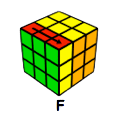
\includegraphics[scale=1.0]{img/Rubik-cube-F.png}
 %\captionsetup{labelformat=empty}
 \caption{魔方的F变换,连续转动4次回到原位。}
 \label{fig:Rubik-cube-F}
%\end{wrapfigure}
\end{figure}

\index{群元素的阶}
我们在前面定义了群的阶,群的元素也可以定义阶。对群中的一个元$a$,能够满足$a^m = e$的最小正整数$m$叫做$a$的阶。如果这样的$m$不存在,我们说$a$的阶是无限的。例如前面例子中魔方旋转群中,$F$旋转4次就回到了原位,所以$F$的阶是4,而$F'$旋转两次回到原位,所以它的阶是2。再比如整数模5的乘法群,除了1以外,其它元素的4次幂都模5余1,所以他们的阶都是4。我们有如下有趣的定理。

\begin{theorem}
有限群的每个元素都有有限的阶。
\end{theorem}

\begin{proof}
如果有限群$G$的阶是$n$,对任意元素$a$,构造集合$\{a, a^2, ..., a^{n+1}\}$。这个集合有$n+1$个元,但是群的阶是$n$,所以根据鸽笼原理,一定有两个元素是相等的, 不妨记这两个元素为$a^i$和$a^j$,其中$0 < i < j \leq n + 1$。我们有:
\[
\begin{array}{rcll}
a^ja^{-i} & = & a^{i}a^{-i} & \text{由} a^i = a^j \\
a^ja^{-i} & = & e & \text{$a^i$和$a^{-i}$互为逆元} \\
a^{j-i} & = & e & a\text{的阶为} j - i
\end{array}
\]
所以$a$的阶为$j-i$是有限的。
\end{proof}

在第一章,我们比较随意地使用了“同构”一词来形容具有相同内在结构的事物。现在我们可以给出同态和同构的概念了。假设存在从某个集合$A$到另一个集合$B$的映射$f$。$a$和$b$是$A$中的两个元,$f(a)$和$f(b)$是它们在$B$中的像。我们考虑$A$上的二元封闭运算产生的元$a \cdot b$,在映射下在$B$中的像$f(a \cdot b)$。如果对$B$上的二元封闭运算总有

\[
f(a) \cdot f(b) = f(a \cdot b)
\]

\begin{figure}[htbp]
\centering
\begin{tikzpicture}[scale=0.8]
\draw (0, 0) circle[x radius=1cm, y radius=3cm]
      (5, 0) circle[x radius=1cm, y radius=3cm];
\path (0, 3) node[above] {$A$:自然数乘法半群}
      (5, 3) node[above] {$B$:平方数乘法半群};
\path (0, 0) node (b) {}
      (5, 0) node (fb) {}
      (0, 1.5) node (a) {}
      (5, 1.5) node (fa) {}
      (0, -1.5) node (c) {}
      (5, -1.5) node (fc) {};
\filldraw (0, 0) circle (1pt) node[above] {$b$}
      (5, 0) circle (1pt) node[above] {$f(b)$}
      (0, 1.5) circle (1pt) node[above] {$a$}
      (5, 1.5) circle (1pt) node[above] {$f(a)$}
      (0, -1.5) circle (1pt) node[above] {$ab$}
      (5, -1.5) circle (1pt) node[above] {$f(ab)$};
\draw[dashed, ->] (b) to node [above] {$f: x \to x^2$} (fb)
      (a) to [bend left] (fa)
      (c) to [bend right] (fc);
\end{tikzpicture}
\[
\begin{array}{rl}
a = 2 & f(a) = 4 \\
b = 3 & f(b) = 9 \\
ab = 6 & f(ab) = f(a)f(b) = 36
\end{array}
\]
\caption{同构}
\label{fig:isomorphism}
\end{figure}

\index{同态映射(homomorphism)}
我们就说$f$是从$A$到$B$的\textbf{同态映射}(homomorphism)。如果$f$是满射(surjection,即$B$中所有元素都在$A$中有原像),则称为同态满射。举一个例子,考虑一个奇偶判定函数$odd: Z \to Bool$,它接受一个整数,如果是奇数就返回真值True,否则返回假False。整数在加法下构成一个群。而布尔集合$\{True, False\}$在逻辑异或运算下也构成一个群。我们可以很容易验证:

\begin{enumerate}
\item $a$和$b$都是奇数,$odd(a)$和$odd(b)$都为真。它们的和是偶数,$odd(a+b)$为假。满足$odd(a) \oplus odd(b) = odd(a+b)$;
\item $a$和$b$都是偶数,$odd(a)$和$odd(b)$都为假。它们的和也是偶数,$odd(a+b)$也为假。满足$odd(a) \oplus odd(b) = odd(a+b)$;
\item $a$和$b$一奇一偶,$odd(a)$和$odd(b)$一真一假。它们的和为奇数,$odd(a+b)$为真。满足$odd(a) \oplus odd(b) = odd(a+b)$;
\end{enumerate}

\index{同构(isomorphism)}
\index{自同构(automorphism)}
如果$f$不仅是满射,还是单射(injection)。那么它就是一一映射。这种情况下,我们称$f$是从$A$到$B$的同构映射,简称\textbf{同构}(isomorphism)。记为$A \cong B$。同构是一种非常强大的关系,不仅两个群可以同构,半群、幺半群以及其它代数结构也可以同构,如图\ref{fig:isomorphism}所示。如果$A$和$B$同构,那么抽象地来看,它们没有什么区别,只有命名上的不同。如果$A$上有一个代数性质,那么在$B$上也有一个完全类似的性质\cite{ZhangHeRui1978}(25页)。另外,$A$与$A$之间的同构映射称为$A$的\textbf{自同构}(automorphism)。例如整数加群在取相反数下成为自同构。

%% \begin{figure}[htbp]
%% \centering
%% \begin{tikzpicture}
%% \path (0, 0) node[below] {猫}
%%       (0, 2) node[above] {羊}
%%       (-2, 2) node[above] {狗}
%%       (-2, 0) node[below] {牛};
%% \filldraw (0, 0) circle (4pt) node (cat) {} --
%%    (0, 2) circle (4pt) node (sheep) {} --
%%    (-2, 2) circle (4pt) node (dog) {} --
%%    (-2, 0) circle (4pt) node (cow) {};
%% \draw (dog) -- (cat) -- (cow);

%% \filldraw[fill=gray, draw=black, pattern=north west lines]
%%     (3, 0) circle (4pt) node (collar) {} --
%%     (5.6, 0) circle (4pt) node (bell) {} --
%%     (4.3, 2.3) circle (4pt) node (milk) {} -- (collar) --
%%     (4.3, 1) circle (4pt) node (wool) {} -- (bell);
%% \path (3, 0) node[below] {项圈}
%%       (5.6, 0) node[below] {铃铛}
%%       (4.3, 2.3) node[above] {奶}
%%       (4.3, 1) node[below] {毛};

%% \draw[dashed, ->] (dog) .. controls (-2.5, 1.5) .. (collar)
%%     (sheep) to[bend left] (wool)
%%     (cat) to[bend right] (bell)
%%     (cow) .. controls (-3, 3) ..(milk);
%% \end{tikzpicture}
%% \[
%% \begin{array}{rl}
%% f(狗) = 项圈 & f(猫) = 铃铛 \\
%% f(羊) = 毛 & f(牛) = 奶
%% \end{array}
%% \]
%% \caption{图的同构(graph isomorphsim)具有不同的定义。它反映了看似不同的两个图,具有相同的结构。}
%% \label{fig:graph-isomorphism}
%% \end{figure}

面对群这种抽象的代数结构时,具体的例子可以帮助我们理解。我们会不自觉地选出一个自己熟悉的代表,例如整数加群,然后看看各种概念,性质在其上是怎样的。但有时这容易形成一种错觉。感觉群的元素大多是一些实体,例如各种数;并且二元运算大多像普通加法、乘法那样可以交换。我们接下来介绍的“变换群”是一个例外,一方面,它不是阿贝尔群,运算不可交换;另一方面群元素不是数,而是变换。

所谓变换,就是一个集合$A$到$A$自身的映射。记为$\tau : A \to A$。它把集合$A$的元素$a$映射为$\tau(a)$,即$a \to \tau(a)$。一个集合可以有多个不同的变换,例如下面是布尔集合的全部变换,我们记真为$T$、假为$F$。

\[
\begin{array}{rll}
\tau_1 : & T \to T, & F \to T \\
\tau_2 : & T \to F, & F \to F \\
\tau_3 : & T \to T, & F \to F \\
\tau_4 : & T \to F, & F \to T
\end{array}
\]

其中变换$\tau_3$和$\tau_4$是一一变换。针对一个集合$A$,我们将它的全体变换放到一起构成一个新的集合:

\[
S = \{\tau, \lambda, \mu, ...\}
\]

现在我们要规定一个S的二元代数运算,把它叫做乘法。为了方便起见,我们将$\tau(a)$用另一个符号表达:

\[
\tau: a \to a^\tau = \tau(a)
\]

这里$a^\tau$不是$a$的$\tau$次方的意思,它只是一个符号记法,表示变换的意思。我们观察$S$的两个元$\tau$和$\lambda$,

\[
\tau: a \to a^\tau,  \lambda: a \to a^\lambda
\]

那么$a \to (a^\tau)^\lambda = \lambda(\tau(a))$显然也是$A$的一个变换,现在我们规定把这个变换叫做$\tau$和$\lambda$的乘积。

\[
\tau\lambda: a \to (a^\tau)^\lambda = a^{\tau\lambda}
\]

读者不妨从前面布尔变换的集合里取几个变换来计算它们的乘积,不难验证这一乘法适合结合律,因为:

\[
\begin{array}{rl}
\tau(\lambda\mu): & a \to (a^\tau)^{\lambda\mu} = ((a^\tau)^\lambda)^\mu \\
(\tau\lambda)\mu: & a \to (a^{\tau\lambda})^\mu = ((a^\tau)^\lambda)^\mu
\end{array}
\]

现在不难看出当初我们选择乘方符号来表达变换的好处了。选择一套强大的符号系统是多年来数学发展的传统和法宝。欧拉、莱布尼茨都是选择和使用符号的大师。对这个乘法来说,$S$的单位元就是$A$的恒等变换$\epsilon: a \to a$。不难验证:

\[
\begin{array}{rl}
\epsilon\tau: & a \to (a^\epsilon)^\tau = a^\tau \\
\tau\epsilon: & a \to (a^\tau)^\epsilon = a^\tau
\end{array}
\]

所以$\epsilon\tau = \tau\epsilon = \tau$。这样$S$对这个乘法来说差不多已经构成一个群了。可惜,虽然说是差不多,到底还是差一点。因为任意变换$\tau$不一定有逆元。例如布尔变换集合中的$\tau_1$,它把任何布尔值都变换成真,不管用这4个变换中的哪一个,都无法把$\tau_1$变换回去。所以$\tau_1$没有逆元。

虽然$S$无法构成群,但是峰回路转,是它的一个子集$G$却有可能构成群。事实上,如果$G$只包含$A$的一一变换,则它在这个乘法下构成群。

\index{变换群(transformation group)}
我们称,一个集合$A$的若干个一一变换对于上述规定的乘法所作成的群叫做$A$的一个\textbf{变换群}(transform group)。并且我们有以下重要的定理:

\begin{theorem}
一个集合$A$的所有一一变换构成一个变换群$G$。
\end{theorem}

变换群一般不是交换群(阿贝尔群),我们可以很容易地找到反例。考虑$\tau_1$是平面上的平移,它把原点(0, 0)移动到(1, 0),变换$\tau_2$是绕原点旋转$\pi/2$,但是:

\[
\begin{array}{rl}
\tau_1\tau_2: & (0, 0) \to (0, 1) \\
\tau_2\tau_1: & (0, 0) \to (1, 0)
\end{array}
\]

\begin{figure}[htbp]
\centering
\begin{tikzpicture}[scale=1]
\draw[->] (-0.5, 0) -- (2, 0) node[right] (x axis) {$x$};
\draw[->] (0, -1.5) -- (0, 1.5) node[above] (y axis) {$y$};
\path (0, -1) node[left] {$a$}
      (1, -1) node[right] {$b$}
      (1, 1) node[above] {$c$};
\filldraw (0, -1) circle(1pt) node (a) {}
          (1, -1) circle(1pt) node (b) {}
          (1, 1) circle(1pt) node (c) {};
\draw[dashed, ->] (a) -- (b);
\draw[dashed, ->] (b) .. controls (1.4, 0) .. (c);
\draw (0, 0) -- (1.2, -1.2)
      (0, 0) -- (1.2, 1.2)
      (1, 0) arc (0:45:1)
      (1, 0) arc (0:-45:1);

\draw[->] (3.5, 0) -- (6.5, 0) node[right] (x axisr) {$x$};
\draw[->] (4, -1.5) -- (4, 1.5) node[above] (y axisr) {$y$};
\filldraw (4, -1) circle (1pt) node[left] (a1) {$a$}
      (5, 0) circle (1pt) node[above] (b1) {$b'$}
      (6, 0) circle (1pt) node[above] (c1) {$c'$};
\draw[dashed, ->] (a1) .. controls (4.7, -0.7) .. (b1);
\draw[dashed, ->] (b1) -- (c1);
\draw (5, 0) arc (0:-90:0.8);
\end{tikzpicture}
\caption{变换顺序不同,结果也不同的例子}
\label{fig:transform-not-abelian}
\end{figure}

因此这一变换群不是阿贝尔群。变换群应用极广,十分重要,我们有一个很强的结论:

\begin{theorem}
任何一个群都同一个变换群同构。
\end{theorem}

我们这里略去了证明过程。这个定理告诉我们,任意一个抽象的群都能在变换群里找到一个具体的实例。换一句话说,我们不必害怕,将来会找到一个抽象群,这个群完全是我们脑子里造出来的空中楼阁\cite{ZhangHeRui1978}(49页)。

\begin{Exercise}
\Question{奇偶判断函数在整数加群$(Z,+)$和布尔逻辑与群$(Bool, \land)$下是否构成同态?去除0元素的整数乘法群呢?}
\Question{假定两个群$G$和$G'$在映射下同态,群$G$中的元$a \to a'$,那么$a$和$a'$的阶是否相同?}
\Question{证明一个变换群的单位元一定是恒等变换。}
\end{Exercise}

\subsection{置换群}
\label{permutation group}
\label{symmetric group}
\index{置换群} \index{对称群}

我们现在介绍$S_2$、$S_3$所在的群家族——置换群。伽罗瓦利用它们思考方程根的对称性,并最早将它们命名为“群”。它们是变换群的一种特例。我们首先定义置换的概念。一个有限集合的一一变换叫做一个\textbf{置换}。一个有限集合的若干个置换作成的一个群叫做一个\textbf{置换群}(permutation group,它相当于对集合的元素进行重新排列)。进一步,一个包含$n$个元素的集合的全体置换作成的群叫做$n$次\textbf{对称群}(symmetric group)。这个群用$S_n$来表示。

由高中的排列组合我们知道,$n$个元素的排列一共有$n!$个。所以对称群$S_n$的的阶是$n!$。一个置换把集合的元素$a_i$变换为$a_j$,我们可以把每个元素置换前后位置的编号按顺序列列出来:$(1, k_1), (2, k_2), ..., (n, k_n)$,或者写成两行的形式:

\[
\begin{pmatrix}
1 & 2 & ... & n \\
k_1 & k_2 & ... & k_n
\end{pmatrix}
\]

例如

\[
\begin{pmatrix}
1 & 2 & 3 & 4 & 5 \\
2 & 5 & 4 & 3 & 1
\end{pmatrix}
\]

就表示了一个置换。明显这样第一行总是$1, 2, ..., n$的形式,所以可以进一步将置换的记法简化为$(2, 5, 4, 3, 1)$。表示原来第1个元素的位置,置换后变成了2个元素;原来第2的位置上,现在变成了第5个元素等等。我们可以按照这种方法列出3个元素集合的全部置换,也就是$S_3$群的元素:

\[
(1, 2, 3), (1, 3, 2), (2, 1, 3), (2, 3, 1), (3, 1, 2), (3, 2, 1)
\]

计算乘法,也就是两个置换的复合时,我们可以这样确定每个位置上元素。针对第$i$个位置,我们先看在第一个置换上它被映射到几,例如$j$,然后再到第二个置换中看第$j$个位置被映射到哪里,例如$k$,这样乘法的结果中,第$i$个位置上的元素就是$k$。我们可以进一步取两个元素相乘,举例看一下$S_3$是否是可交换的:

\[
\begin{array}{l}
(1, 3, 2) (2, 1, 3) = (2, 3, 1) \\
(2, 1, 3) (1, 3, 2) = (3, 1, 2)
\end{array}
\]

所以$S_3$不是阿贝尔群。它是一个最小的有限非阿贝尔群。一个有限非阿贝尔群至少要有6个元素。我们观察5个元素的一个置换$(2, 3, 1, 4, 5)$,发现只有前三个元素变化了,而后两个元素保持不变。而前三个元素的变化很有特点,如图\ref{fig:cycle-permutation}所示,恰好是循环地画了个圈。

\begin{figure}[htbp]
\centering
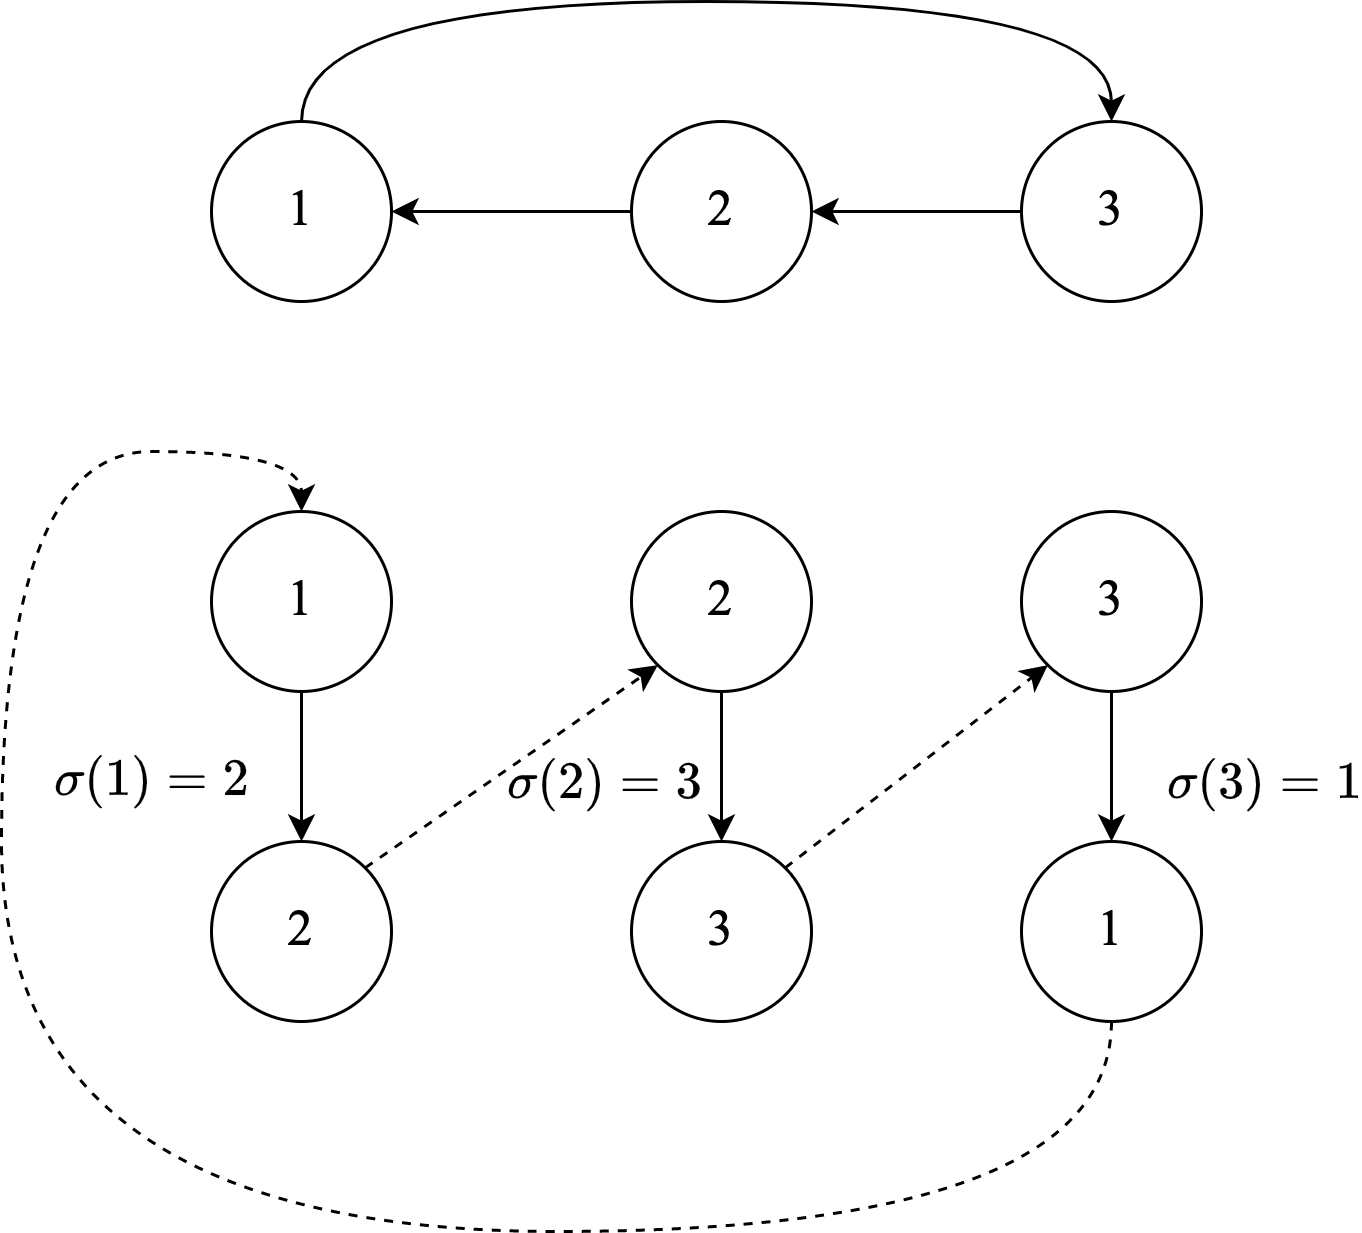
\includegraphics[scale=0.6]{img/3-cycle}
\caption{3循环置换$(1\ 2\ 3)$}
\label{fig:cycle-permutation}
\end{figure}

为此我们可以把置换$(2, 3, 1, 4, 5)$进一步简写为$(1\ 2\ 3)$。注意这种写法元素间没有逗号,并且认为$(1\ 2\ 3)$、$(2\ 3\ 1)$、$(3\ 1\ 2)$都表示同一个3循环置换\footnote{如果少于10个元素,也可用不带空格的$(123)$来表示。超过10个时应加入空格避免歧义,如:$(12\ 3)$}。这种记法称为$k$-循环置换,表示$k$个元素组成一个循环:$(i_1\ i_2\ ...\ i_k)$,它将每个元素映射成下一个元素,最后一个元素映射成第一个元素:

\[
i_1 \to i_2 \to i_3, ..., i_{k-1} \to i_k \to i_1
\]

这个解释用的是映射的观点,如图\ref{fig:cycle-permutation}下方所示。令置换为$\sigma$,按照图中箭头的顺序:$1 \to \sigma(1) = 2$, $2 \to \sigma(2) = 3$,$3 \to \sigma(3) = 1$。另一种解释使用移动的观点,$k$-循环置换把后一个元素移动到前一个的位置,第一个元素移动到最后,组成循环,如图\ref{fig:cycle-permutation}上方所示。$k$-循环的元素并不一定相邻,例如$(3\ 9\ 4)$,也不一定有固定的顺序,例如$(2\ 4\ 1\ 3)$。如果循环只有两个元素$(i\ j)$称其为对调(transposition)。有个特殊情况,就是恒等置换,我们把它记为$e = (1)$。并且有:

\[
e = (1) = (2) = ... = (n)
\]

现在我们观察置换$(2, 1, 4, 5, 3)$,它有两个循环,一个是2循环置换$(1\ 2)$,另一个是3循环置换$(3\ 4\ 5)$。为此我们可以将它表示为两个置换的乘法:

\[
(2, 1, 4, 5, 3) = (1\ 2)(3\ 4\ 5)
\]

事实上,每一个$n$元的置换$\pi$都可以写成若干个互相没有共同数字的循环置换的乘积。采用这种方法的好处是,虽然一般的置换是不可交换的,但是由于$k$-循环置换彼此没有共同数字,所以它们是可交换的。例如$(1\ 2)(3\ 4\ 5) = (3\ 4\ 5)(1\ 2)$。下面是$S_3$的全体循环置换用这种记法的列表,1个恒等,3个对调,2个循环(顺、逆时针):

\[
(1), (1\ 2), (1\ 3), (2\ 3), (1\ 2\ 3), (1\ 3\ 2)
\]

任给一个置换$(k_1, k_2, ..., k_n)$,如何将其转化为若干个不相连的循环置换乘积呢?我们可以按照这样的规则来操作。首先从左到右依次比较置换的每个元素,如果$k_i$和$i$相等,说明这个元素无需置换;否则先写下左括号,然后将第$k_i$个元素的值$k_j$写到括弧中,接着顺着$k_j$继续寻找,将其和$j$比较,如果不等,就写入括弧。重复这个步骤直到发现某个元素形成了循环,此时$k_i = i$。这时可以写下右括号,完成一个循环。此后再继续从左向右比较置换中的元素,直到处理完所有的\cite{Armstrong1988}(27页)。如果所有的$k_i$都和$i$相等,我们可以写下$(1)$表示恒等置换。这一过程特别适合用编程的方法实现,下面是相应的算法。

\begin{algorithmic}[1]
\Function{k-cycles}{$\pi$}
  \State $r \gets [\ ], n \gets |\pi|$
  \For{$i \gets 1$ to $n$}
    \State $p \gets [\ ], j \gets i$
    \While{$j \neq \pi[j]$}
      \State $p \gets p \doubleplus [j]$
      \State $j \gets \pi[j]$
    \EndWhile
    \If{$p \neq [\ ]$}
      \State $r \gets r \doubleplus [p]$
    \EndIf
  \EndFor
  \If{$r \neq [\ ]$}
    \State \Return r
  \Else
    \State \Return $[[1]]$ \Comment{返回恒等变换}
  \EndIf
\EndFunction
\end{algorithmic}

由上一小节的定理,我们有

\begin{theorem}
每一个有限群都与一个置换群同构。
\end{theorem}

这样对于任何有限群,例如方程的根,我们都可以用置换群加以研究。而置换群又是一种比较容易计算的群,这正是伽罗瓦解决方程根式解问题的方法。

\begin{Exercise}
\Question{证明,如果置换$\sigma$将第$i$个元素映射为第$j$个,即$\sigma(i) = j$,则$k$循环可写成$(\sigma(i_1)\ \sigma(\sigma(i_1))\ ...\ \sigma^k(i_1))$。}
\Question{列出$S_4$的全体元素。}
\Question{将$S_3$的所有元写成不相连的循环置换的乘积。}
\Question{编程将$k$-循环的乘积转换回置换。}
\end{Exercise}

\subsection{群与对称}

为什么包含集合元素的全体置换作成的群叫做“对称群”呢?因为这个群揭示了对称的本质。我们考虑一个正三角形的对称性。记正三角形的三个顶点为1、2、3,我们取$S_3$中的三个元素(1 2), (1 2 3)和(1 3 2)对正三角形进行变换:

\begin{figure}[htbp]
 \centering
 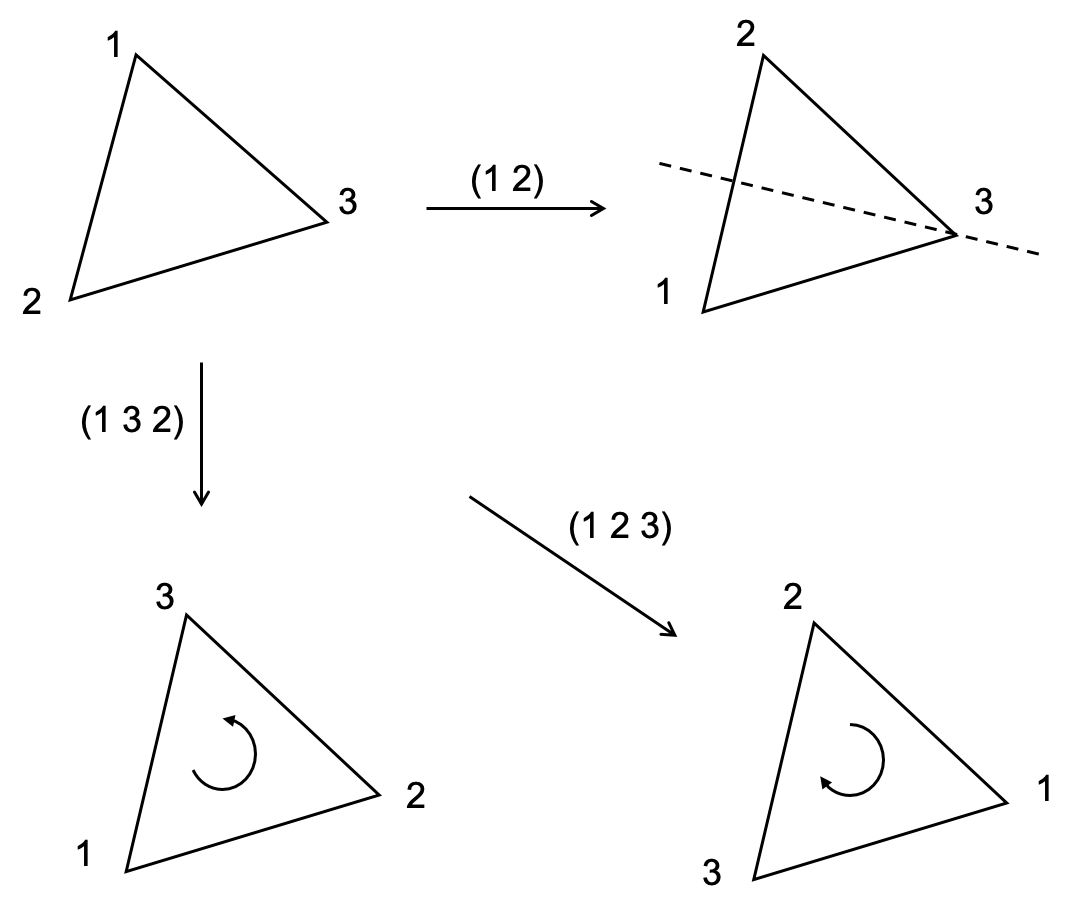
\includegraphics[scale=0.4]{img/s3-examples.png}
 %\captionsetup{labelformat=empty}
 \caption{正三角形的对称变换}
 \label{fig:S3-examples}
\end{figure}

\begin{enumerate}
\item 图中右侧图形是(1 2)变换的结果,三角形的三个顶点从123变为213,它恰恰是以过点3的对称轴进行翻转变换的结果。由于变换前后的图形重合,这说明正三角形是轴对称的。除了(1 2)外,它还有另外两个轴对称,分别对应群元素(1 3)、(2 3)。相应的对称轴是过点2和点1的高。

\item 图中右下是(1 2 3)变换的结果。三角形的三个顶点从123变为231。它等价于绕中心顺时针旋转120度。由于变换前后图形重合,这说明正三角形具有120度旋转对称性。

\item 图中下方是(1 3 2)变换的结果。三角形的三个顶点从123变为312。它等价于绕中心逆时针旋转120度,或者顺时针旋转240度。由于变换后图形重合,这说明正三角形具有240度旋转对称性。
\end{enumerate}

这样正三角形的每种对称性(3个轴对称、加上2个旋转对称性,以及恒等变换)恰好被对称群$S_3$的每个元素唯一精确描述了。这就是群与对称间的美妙关系。

我们把这些不改变物体大小的变换称为叠合。存在着两种叠合,一种称为真叠合(proper)一种称为非真叠合(improper)。为什么会有这种差别呢?考虑下面图中的两种海螺,左边的那种多在北半球发现,右边的那种多在南半球发现。尽管它们摆在一起如此对称,我们却发现无论怎样旋转、翻转、移动,都无法让左侧的海螺和右侧的完全相合。左侧的海螺是左螺旋的,而右侧的是右螺旋的。两个互为镜像。

\begin{figure}[htbp]
 \centering
 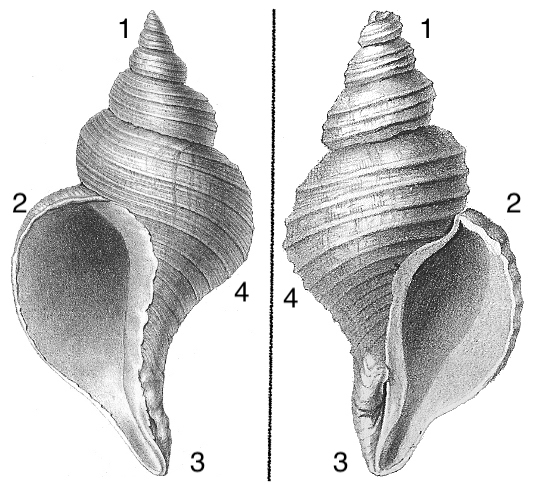
\includegraphics[scale=0.3]{img/chirality.jpg}
 %\captionsetup{labelformat=empty}
 \caption{真叠合与非真叠合}
 \label{fig:chirality}
\end{figure}

在现实世界中,我们无法通过运动将左螺旋变成镜子中的右螺旋。这就是真与非真叠合的区别:真叠合不改变螺旋的方向,将左螺旋变为左螺旋,右螺旋变为右螺旋;非真叠合改变螺旋的方向,将左螺旋变为右螺旋,右螺旋变为左螺旋。非真叠合又称为反射\cite{Weyl1952}。它把任一点$P$变成它关于$O$点的对应点$P'$:先连接$PO$,然后将其延长一倍使得$|PO| = |OP'|$。对$O$的反射,通常也称为反演。
对于海螺图中的4点,对称群$S_4$中的变换(2 4)就是一个非真叠合。它将左侧的海螺变换成右侧的。因此对称群既可以描述现实世界,也可以描述镜中世界的对称。

\begin{Exercise}
对称群$S_4$描述了什么几何形状的哪些对称性?
\end{Exercise}

\subsection{旋转对称与循环群}
\index{循环群(cyclic group)}

\begin{figure}[htbp]
 \centering
 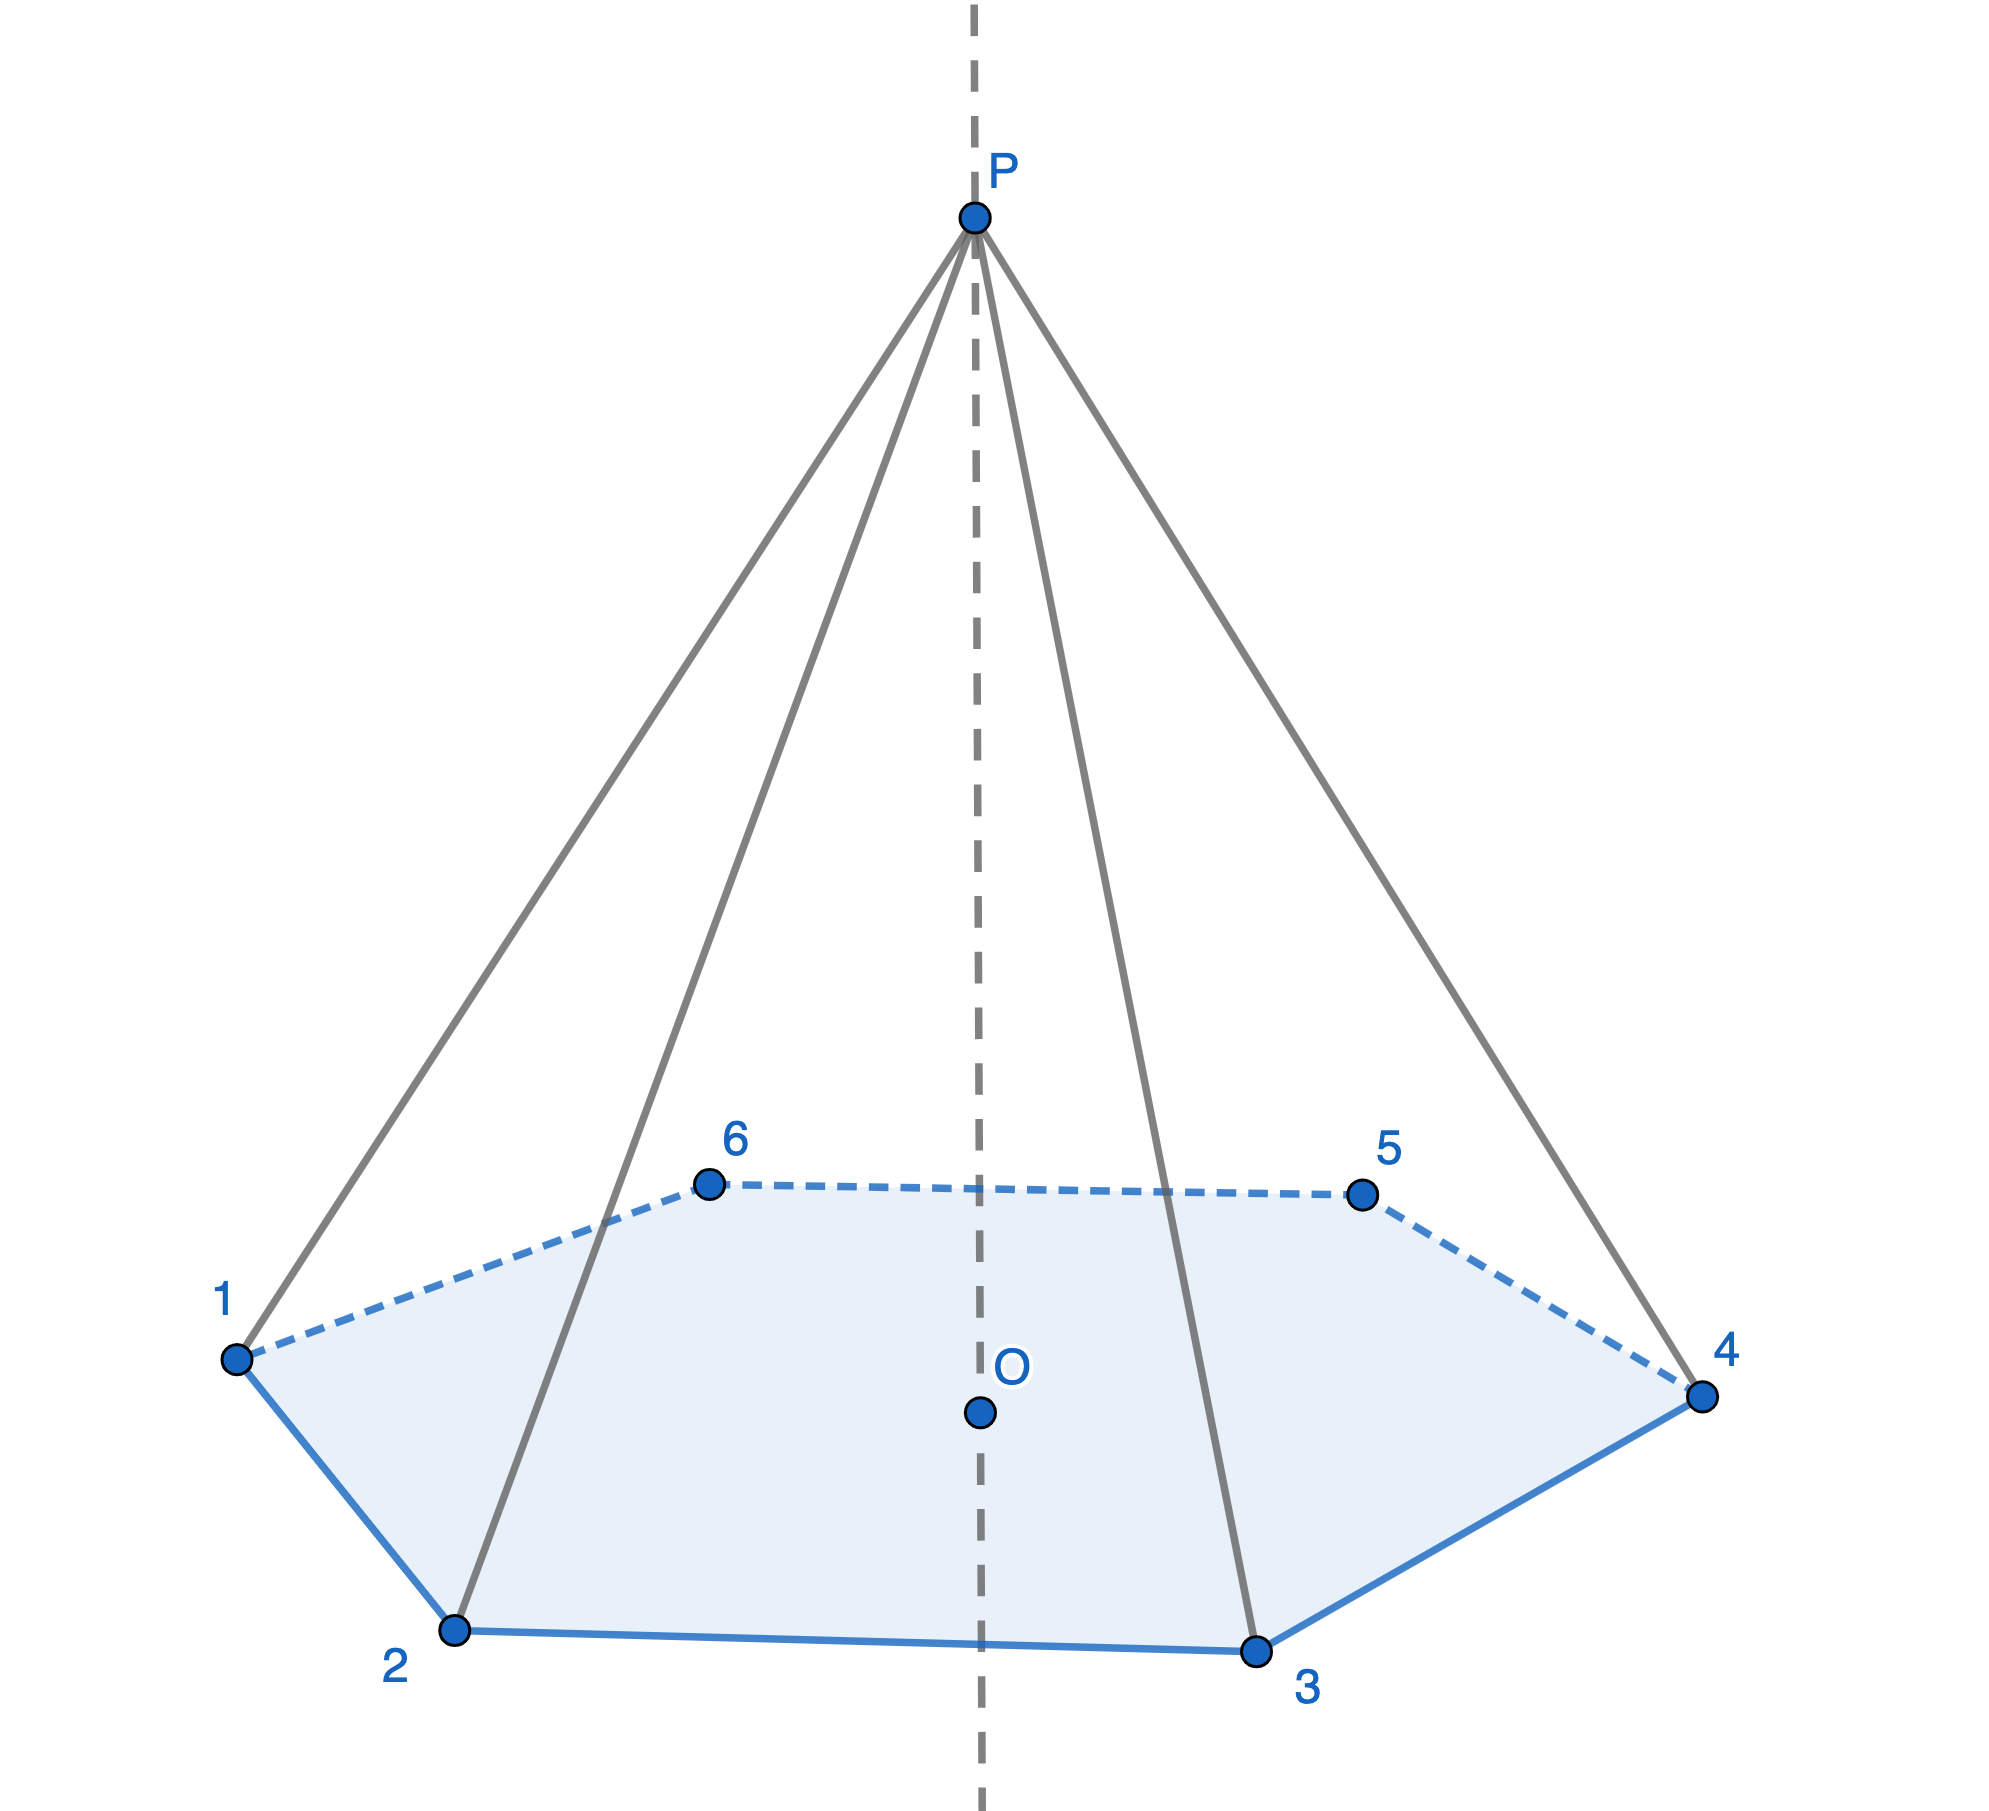
\includegraphics[scale=0.8]{img/hexagonal-pyramid.png}
 \caption{正六棱锥}
 \label{fig:regular-hexagonal-pyramid}
\end{figure}

正六棱锥也是对称的,它围绕通过锥顶垂直底面的对称轴OP旋转60度、120度、180度、240度、300度、360度和这些度数的整数倍和自己重合。我们称这种对称为旋转对称\footnote{除旋转对称外,正六棱锥还有镜面对称,过中心轴和任意边中点的3个对称平面,过中心轴和底面顶点的3个对称平面。}。虽然底面的正六边形有6个端点,但$S_6$并非描述正六棱锥对称性的群。$S_6$有$6! = 720$个置换,但正六棱锥本质上只有6种旋转对称。如果定义绕中心轴旋转60度为$r$,旋转120度相当于旋转60度后再次旋转60度,即:$r \cdot r = r^2$,类似的旋转180度相当于$r^3$……旋转360度后恢复原位,所以$r^6 = e$。这样描述六棱锥旋转对称性的变换集合包含6个元素:$C_6 = \{e, r, r^2, r^3, r^4, r^5\}$。不难验证它们构成一个群,并且同构于$S_6$的子集$\{(1), (1\ 2\ 3\ 4\ 5\ 6), ..., (5\ 6\ 1\ 2\ 3\ 4)\}$。比较$C_6$和$S_3$,虽然它们都含有6个元素,可是这两个群的结构是不同的,$S_3$并不能描述六棱锥的旋转对称性。

$C_6$只是一个代表,它也是一族群中的某个成员。我们可以想像出$C_n$这样的群以描述正$n$棱锥的旋转对称性。这种群称为循环群(cyclic group)。他是最简单的,人们已经完全解决了的一类群。一个群$G$中的所有元素都是某一个固定元素的乘方。例如,我们看去掉0元素的模5乘法群。它包含4个元素\{1, 2, 3, 4\},其中2的各个乘方模5的结果如下:

\[
\begin{array}{l}
2^1 \bmod 5 = 2 \\
2^2 \bmod 5 = 4 \\
2^3 \bmod 5 = 3 \\
2^4 \bmod 5 = 1
\end{array}
\]

所以2的乘方生成了这个群中的所有元素。为此我们定义:

\begin{definition}
若一个群的每个元素都是某个固定元素$a$的乘方,称$G$为\textbf{循环群}。我们也说,$G$是由元$a$所生成的,并且用符号

\[
G = (a)
\]

来表示,$a$叫做$G$的一个生成元。
\end{definition}

我们举两个循环群的重要例子:

\begin{example}
整数加群中的全体整数都是1的“乘方”,这里的二元运算是加法,所以乘方就是不断进行相加。我们看任意正整数$m$:

\[
\begin{array}{rcll}
1^m & = & 1 \cdot 1 \cdot 1 \cdot ... \cdot 1 & \text{$m$次} \\
    & = & 1 + 1 + ... + 1 & \text{整数加群中乘法为+} \\
    & = & m &
\end{array}
\]

在整数加群中,1的逆元是-1,这是因为1 + (-1) = 0,而0是单位元。所以对任意负整数$-m$有:

\[
\begin{array}{rcll}
1^{-m} & = (-1)^m & \text{逆元} & \\
(-1)^m & = & (-1) \cdot (-1) \cdot (-1) \cdot ... \cdot (-1) & \text{$m$次} \\
       & = & -1 + (-1) + ... + (-1) & \text{整数加群中乘法为+} \\
       & = & -m &
\end{array}
\]

最后0是单位元,按照定义有$0 = 1^0$。综合上述三种情况,我们有$Z = (1)$。
\end{example}

这是一个无限循环群的例子,我们再举一个有限循环群的例子。

\begin{example}
我们看整数模$n$剩余类。我们用符号$[a]$表示整数$a$所在的剩余类。定义二元运算为模$n$的加法。

\[
[a] + [b] = [a + b]
\]

例如[3] + [4] 在模5时,结果为[2]。我们不难验证它符合结合律,单位元是[0],并且每个元素都存在逆。我们把这个群叫做整数模$n$的剩余类加群。包含元素[0], [1], ..., [$n$-1]。这个群是一个循环群,因为每个元[$i$]都可以写成$i$个[1]的乘方。

\[
[i] = [1] + [1] + ... + [1] \quad \text{$i$个}
\]
\end{example}

这两个例子不是随便选的。实际上,由这两个例子,我们已经认识了所有的循环群!因为有如下定理:

\begin{theorem}
若$G$是由元素$a$所生成的循环群,那么$G$的构造完全可以由$a$的阶来决定:
\begin{itemize}
\item 如果$a$的阶无限,那么$G$与整数加群同构;
\item 如果$a$的阶是整数$n$,那么$G$与整数模$n$剩余类加群同构。
\end{itemize}
\end{theorem}

\begin{proof}
如果$a$的阶无限,我们有$a^h = a^k$当且仅当$h = k$。否则,如果$h \neq k$,不妨令$h > k$,我们有$a^{h - k} = e$,这与$a$的阶无限矛盾。所以我们可以构造一一映射:

\[
f: a^k \to k
\]
从而建立循环群$G=(a)$到整数加群$Z$之间的同构。即:$a^ha^k \to h + k$。

如果$a$的阶是整数$n$,即$a^n = e$。这时$a^h = a^k$当且仅当$h \equiv k \mod n$的时候。我们可以构造一一映射:

\[
f: a^k \to [k]
\]

从而建立循环群$G = (a)$到整数模$n$剩余类加群间的同构。即:

\[
a^ha^k = a^{h + k} \to [h + k] = [h] + [k]
\]
\end{proof}

正是这个原因,我们有时把循环群$C_n$写成$\mathbb{Z}/n\mathbb{Z}$。所以,抽象地来看,生成元的阶是无限大的循环群只有一个,生成元的阶是某个正整数的群也只有一个。至于这些循环群的构造,我们也知道得很清楚:

\begin{itemize}
\item $a$的阶无限大
  \begin{itemize}
  \item 群元素是:..., $a^{-2}, a^{-1}, a^0, a^1, a^2$, ...
  \item 群乘法是:$a^ha^k = a^{h + k}$
  \end{itemize}
\item $a$的阶是$n$
  \begin{itemize}
  \item 群元素是:$a^0, a^1, a^2, ..., a^{n-1}$
  \item 群乘法是:$a^ha^k = a^{(h + k) \bmod n}$
  \end{itemize}
\end{itemize}

% https://en.wikipedia.org/wiki/Wilson_Bentley
\begin{figure}[htbp]
 \centering
 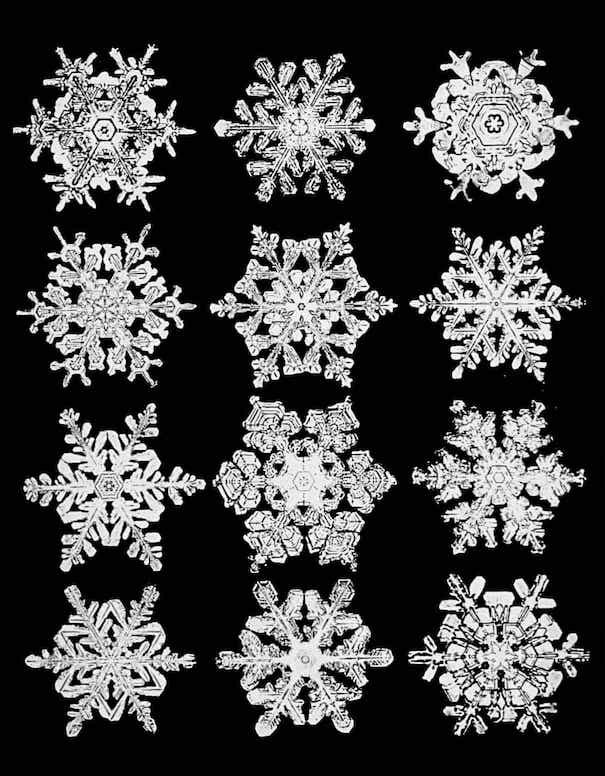
\includegraphics[scale=0.3]{img/snowflakes.jpg}
 \caption{美国摄影家威尔逊$\cdot$本特利于1902年前后拍摄的雪花晶体}
 \label{fig:snowflakes}
\end{figure}


现在我们可以揭示雪花的旋转对称性了。它可以被循环群$C_6$描述。它们表示雪花旋转60度、120度、180度、240度、300度、360度的整数倍和自己重合,每种旋转恰好是6阶循环群中的一个元素。概括地说,$n$阶循环群描述了正$n$边形的旋转对称。正$n$棱柱截面上的旋转对称性也可以用循环群来描述。美国摄影家威尔逊$\cdot$本特利一生拍摄了超过5000张雪花晶体照片。他把这些艺术与科学的结晶捐赠给了博物馆。从这些照片中,他得出了孩子们熟知的结论:“每一片雪花都是不同的。”

\subsubsection{分圆方程}

如果把代表雪花旋转对称性的六边形放到复平面上,将大小缩放到内接于单位圆。我们发现六边形的顶点对应于方程$x^6 - 1 = 0$的六个根。如图\ref{fig:cyclotomic-6}所示。显然$x = \pm 1$是方程的两个解。剩下的解是什么呢?根据高中数学中的棣莫弗公式:

\begin{figure}[htbp]
 \centering
 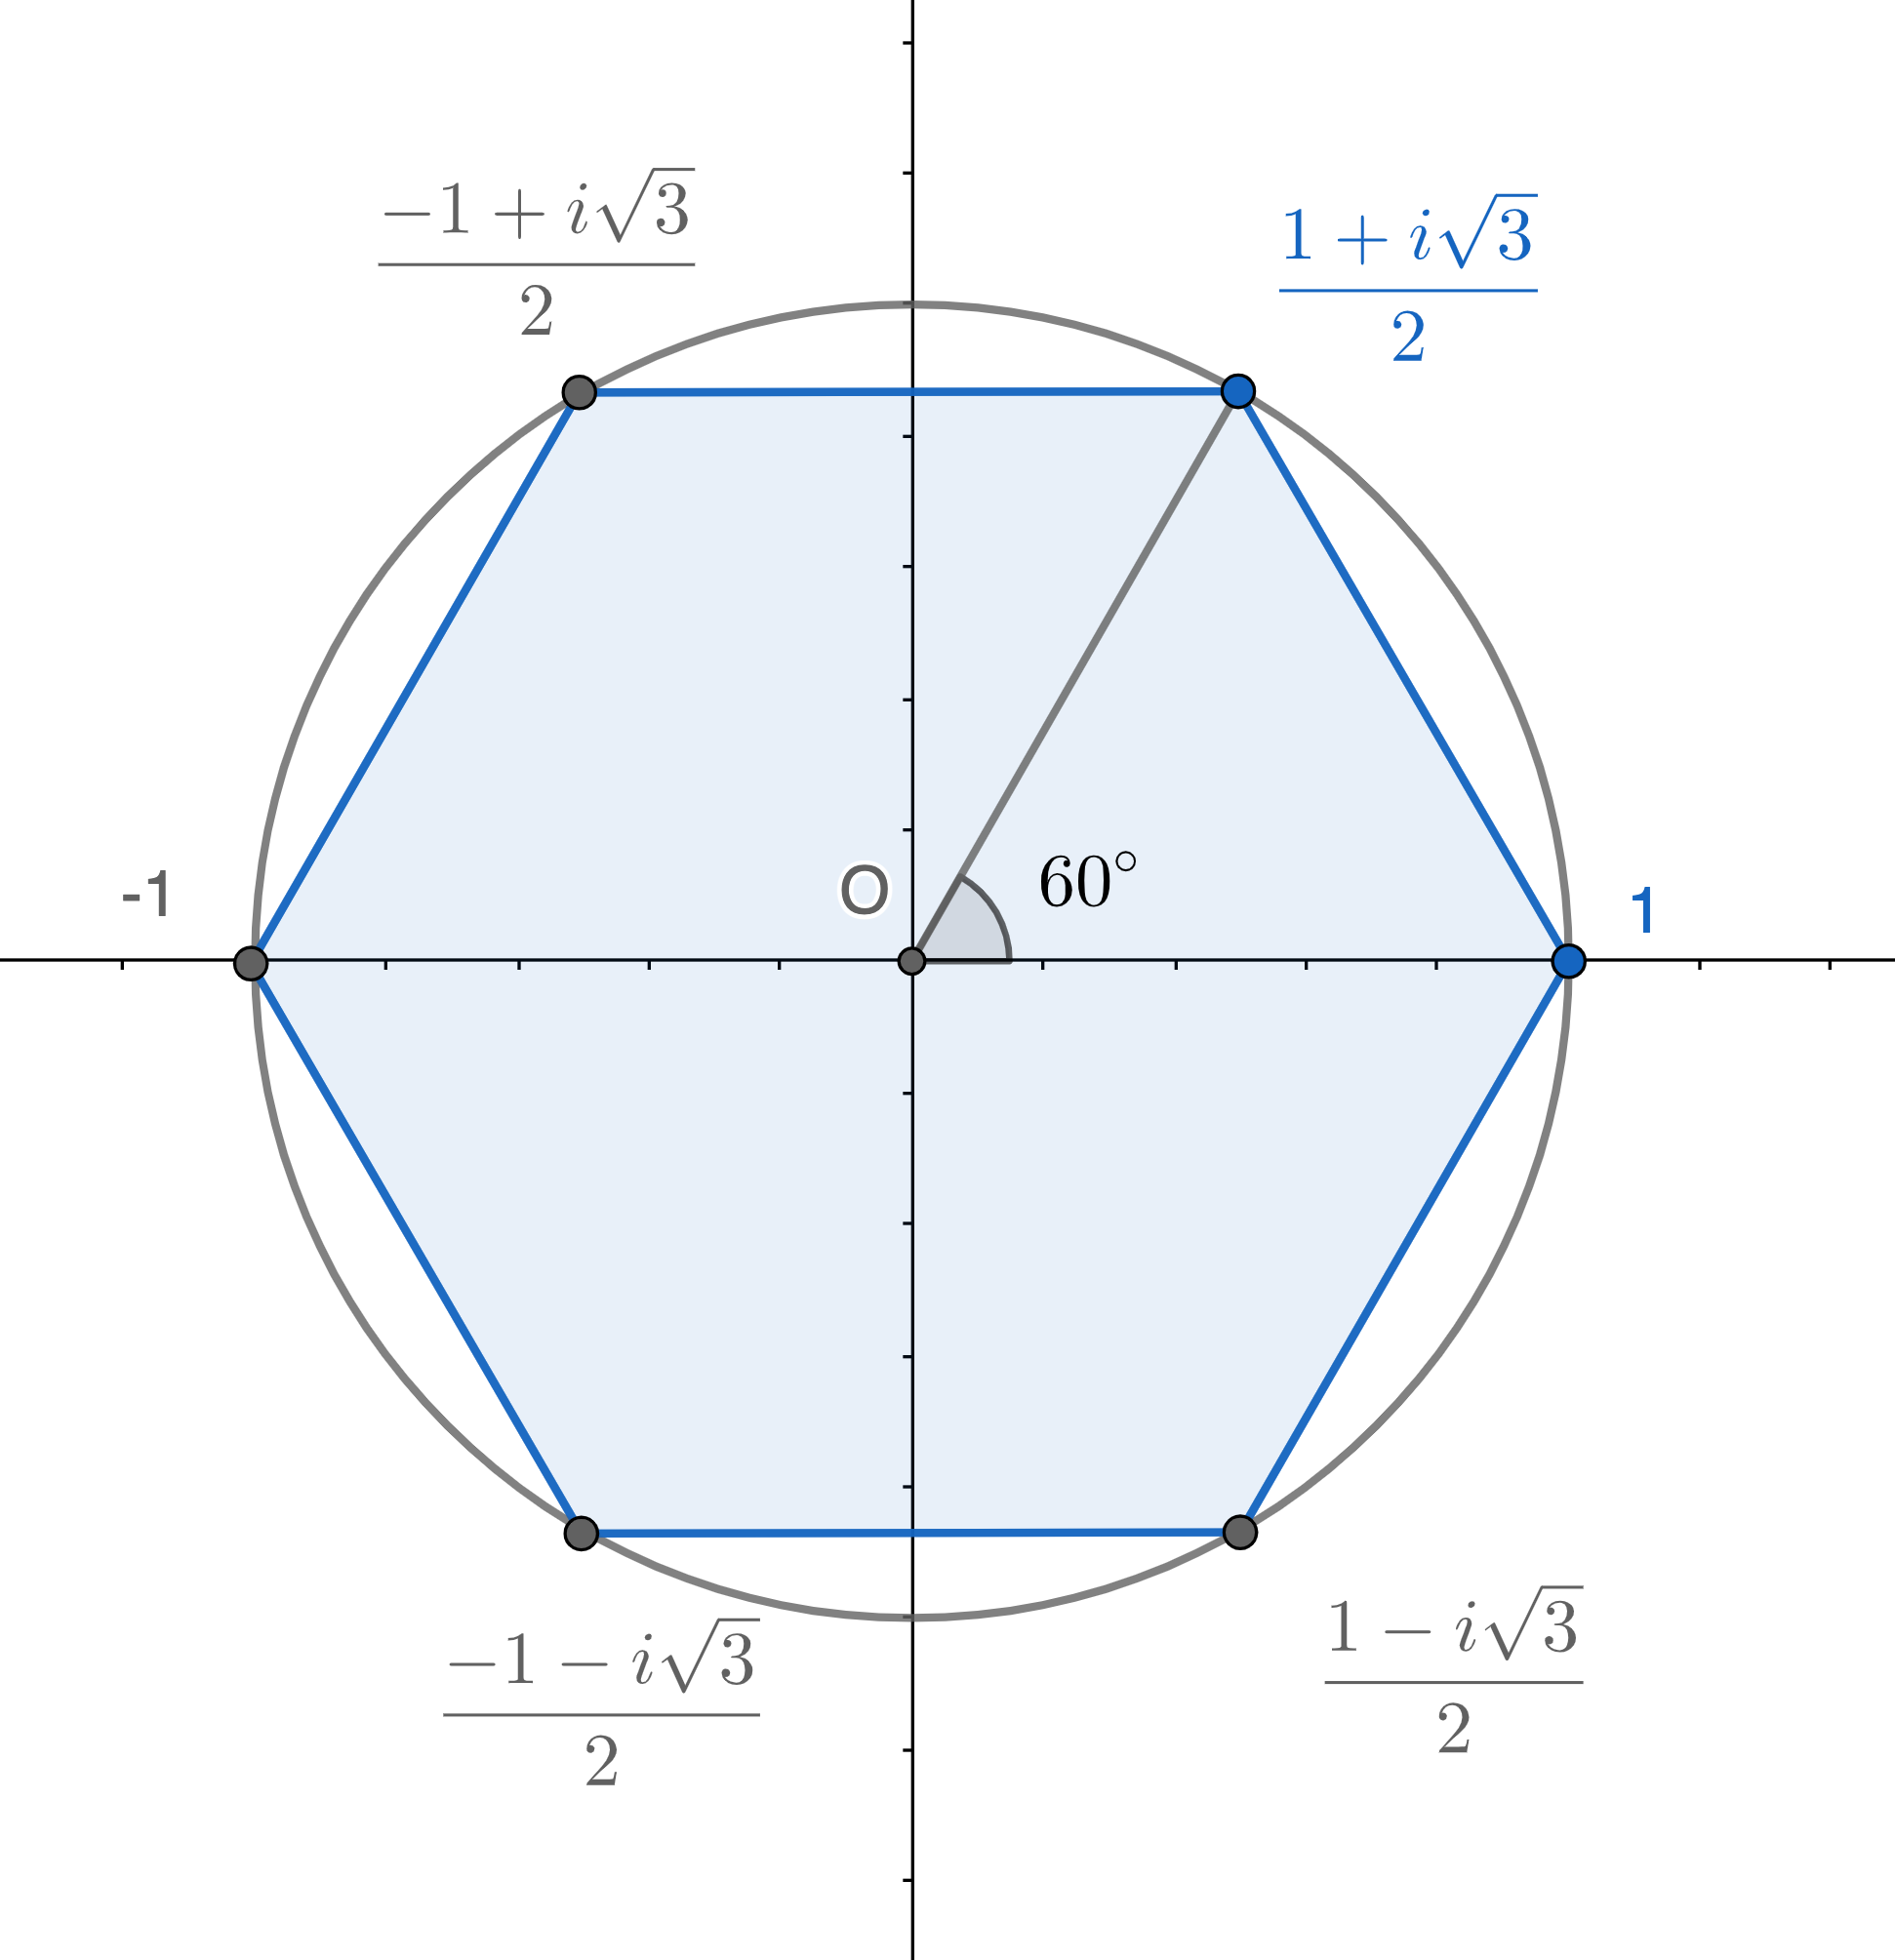
\includegraphics[scale=2]{img/cyclotomic-6.png}
 \caption{$x^6 - 1 = 0$的解}
 \label{fig:cyclotomic-6}
\end{figure}

\be
e^{i n \theta} = \cos n \theta + i \sin n \theta = (\cos \theta + i \sin \theta)^n
\ee

我们可以给出方程的全部6个解为:$\zeta_0 = 1, \zeta_1 = e^{i\frac{\pi}{3}}, \zeta_2 = e^{i\frac{2\pi}{3}}, \zeta_3 = e^{i\pi}, \zeta_4 = e^{i\frac{4\pi}{3}}, \zeta_5 = e^{i\frac{5\pi}{3}}$。它们平均地把单位圆分成6等分。也正是出于这个原因,我们把形如$x^n - 1 = 0$的方程称为“分圆方程”。$n$个解中的每个可以表示为$\zeta_k = e^{i\frac{2k\pi}{n}}$。可是这样的解并非是分圆方程代数解,我们也无从得知是否可以通过尺规作出正$n$边形。我们下面思考$n$等于2, 3, 4, 6, 12时分圆方程的解。

$n = 2$,因式分解$x^2 - 1 = (x + 1)(x - 1)$,所以分圆方程的两个根为$\pm 1$。$n=3$,我们知道$x = 1$是一个根,所以$x^3 - 1$一定可以被$x - 1$整除,我们用多项式除法得到:$x^3 - 1 = (x - 1)(x^2 + x + 1)$。进一步解一元二次方程$x^2 + x + 1 = 0$得到全部的三个解:1、$\dfrac{-1 \pm i \sqrt{3}}{2}$。通常人们命名$\omega = \dfrac{-1 + i \sqrt{3}}{2}$,这样三次分圆方程的根可以记为:$1, \omega, \omega^2$。

\begin{center}
\polylongdiv{x^3-1}{x-1}
\end{center}

$n = 4$,因式分解$x^4 - 1 = (x^2 - 1)(x^2 + 1) = (x - 1)(x + 1)(x - i)(x + i)$。四次分圆方程的四个根分别是$\pm 1, \pm i$。

%% $n = 5$,由于$x - 1$是因子,我们再次用多项式除法$x^5 - 1 = (x - 1)(x^4 + x^3 + x^2 + x + 1)$。为了解方程$x^4 + x^3 + x^2 + x + 1 = 0$,令$y = x + 1/x$,这样就转化为解一元二次方程$y^2 + y - 1 = 0$。得到两个解:$y = \dfrac{-1 \pm \sqrt{5}}{2}$。代回方程$x^2 - yx + 1 = 0$,得到全部五个解:

%% \[
%% 1, \dfrac{\sqrt{5} - 1 \pm \sqrt{-2 \sqrt{5} - 10}}{4},
%%    \dfrac{-\sqrt{5} - 1 \pm \sqrt{2 \sqrt{5} - 10}}{4}
%% \]

$n = 6$,因式分解得$x^6 - 1 = (x^3 - 1)(x^3 + 1)$。所以三次分圆方程的解也全部是6次分圆方程的解。容易验证$x = -1$也是一个解,所以$x^3 + 1$必然含有$(x + 1)$这个因式。利用多项式除法,我们得到:$x^3 + 1 = (x + 1)(x^2 - x + 1)$。进一步解一元二次方程$x^2 - x + 1 = 0$,我们得到6次分圆方程的全部6个解:$\pm 1, \dfrac{\pm 1 \pm i \sqrt{3}}{2}$。如图\ref{fig:cyclotomic-6}所示。

%% \begin{center}
%% \polylongdiv{x^3+1}{x+1}
%% \end{center}

6次分圆方程的解包含3次分圆方程的所有解,这种现象并非特殊。4次分圆方程包含2次分圆方程的所有解,并且6次分园方程也包含2次分圆方程的所有解。这样就引出了两个不同的概念:

\begin{enumerate}
\item $n$次单位根: $n$次方等于1的数,即$x^n = 1$;
\item $n$次本原单位根:$n$次方后第一次等于1的数。即$x^n = 1$,但对于任何$m = 1, 2, ..., n - 1$,都有$x^m \neq 1$。
\end{enumerate}

比如$-1$是2次本原单位根,尽管它也是4次单位根,但它不是4次本原单位根。观察我们对$x^n - 1$分解因式的过程,例如$x^3 - 1 = (x - 1)(x^2 + x + 1)$。这两个因式都不可继续分解了,其中$x - 1$的根是1次本原单位根,而$x^2 + x + 1$的根(两个)是3次本原单位根。我们称它们为分圆多项式。$k$次本原单位根对应的分圆多项式记为$\Phi_k(x)$。分圆方程和分圆多项式之间有一个重要的结论:

\be
x^n - 1 = \displaystyle \prod_{d | n} \Phi_d(x)
\ee

也就是说,整数$n$有哪些因子,$x^n - 1$就可以因式分解为这些因子对应分圆多项式。分圆方程和循环群之间存在有趣的联系:所有$n$次单位根在乘法下构成一个循环群$C_n$,而$n$次本原单位根$\zeta_k$是这个群的生成元,即$C_n = (\zeta_k)$。

\btab{|c|c|c|c|c|c|}
\hline
$n$ & 分圆方程 & 根 & 本原单位根 & 分圆多项式$\Phi_n(x)$ & 循环群 \\
\hline
1 & $x - 1 = 0$ & 1 & 1 & $x - 1$ & $C_1$ \\
\hline
2 & $x^2 - 1 = 0$ & $\pm 1$ & -1 & $x + 1$ & $C_2$ \\
\hline
3 & $x^3 - 1 = 0$ & $1, \omega, \omega^2$ & $\omega, \omega^2$ & $x^2 + x + 1$ & $C_3$ \\
\hline
4 & $x^4 - 1 = 0$ & $\pm 1, \pm i$ & $\pm i$ & $x^2 + 1$ & $C_4$ \\
\hline
6 & $x^6 - 1 = 0$ & $\pm 1, \dfrac{\pm 1 \pm i \sqrt{3}}{2}$ & $\dfrac{1 \pm i \sqrt{3}}{2}$ & $x^2 - x + 1$ & $C_6$ \\
\hline
\etab

\begin{Exercise}
\Question{证明循环群一定是阿贝尔群。}
\Question{证明素数$p$阶的群一定循环群,从而一定是阿贝尔群。}
\label{ex:p-grp-abelian}
\Question{编程实现多项式长除法。}
\Question{将$x^{12} - 1$分解为分圆多项式。}
\Question{试求5次分圆方程的代数解。提示:分圆多项式$x^4 + x^3 + x^2 + x + 1 = 0$除以$x^2$后是对称的:$x^2 + x + 1 + x^{-1} + x^{-2} = 0$。}
% let y = x + 1/x => y^2 + y - 1 = 0
% from: https://crypto.stanford.edu/pbc/notes/numbertheory/cyclo.html
\end{Exercise}

\subsection{子群}
\index{子群}

我们接下来介绍子群的概念。它可以帮助我们通过一个群的子集来推测整个群的性质。

\begin{definition}
一个群$G$的一个子集$H$叫做$G$的一个\textbf{子群},如果$H$对于$G$的乘法也构成一个群。
\end{definition}

对于任何群$G$,至少有两个子群,一个是$G$本身,另外是只包含一个单位元的集合$\{e\}$。这两个子群称为平凡子群。对于整数加群来说,偶数加群构成一个子群,而奇数和加法不构成子群(为什么?)。我们再举一个例子,考虑上一节介绍的置换群$S_3$的子集$H = \{(1), (1\ 2)\}$,$H$在置换复合乘法下构成一个子群。我们下面来验证一下:

\begin{enumerate}
\item 乘法的封闭性。$(1)(1) = (1)$, $(1)(1\ 2) = (1\ 2)$, $(1\ 2)(1) = (1\ 2)$, $(1\ 2) (1\ 2) = (1)$;其中最后一个乘法表示头两个元素对调后再对调会相当于恒等置换。
\item 结合律对$S_3$的所有元素都成立,故对$H$的元素也成立;
\item 单位元$(1) \in H$;
\item 每个元素的逆元都存在:$(1)(1) = (1)$、$(1\ 2) (1\ 2) = (1)$。
\end{enumerate}

这样依次验证群的所有性质比较麻烦,我们有一个方便的工具:

\begin{theorem}
一个群$G$的非空子集$H$构成子群的充分必要条件是:
\begin{enumerate}
\item 若任意$a, b \in H$,则$ab \in H$;
\item 任意元素$a \in H$,有$a^{-1} \in H$。
\end{enumerate}
\label{theorem:subgroup}
\end{theorem}

我们把这一定理的证明留作练习。这个定理可以直接得到一个推论,如果$H$是$G$的子群,那么$H$的单位元就是$G$的单位元,$H$中任意元素$a$的逆元就是它在$G$中的逆元。上述定理中的两个条件也可以用一个合并的条件来代替:

\begin{theorem}
一个群$G$的非空子集$H$构成子群的充分必要条件是。若任意$a, b \in H$,则$ab^{-1} \in H$。
\label{theorem:subgroup-2}
\end{theorem}

\begin{proof}
首先证明充分性,设$a, b \in H$,由上一定理的条件2,有$b^{-1} \in H$。再由条件1,有$ab^{-1} \in H$;

现在反过来证明必要性。设$a \in H$,根据单位元公理$aa^{-1} = e \in H$。因为$e, a \in H$,所以$ea^{-1} = a^{-1} \in H$。这就是前面定理中的条件2;接下来若$a, b \in H$,由刚刚证明的结果,$b^{-1} \in H$。所以$a(b^{-1})^{-1} = ab \in H$。这就证明了前面定理中的条件1。
\end{proof}

假如子集$H$是有限集,那么$H$构成子群的条件要更简单:

\begin{theorem}
一个群$G$的非空有限子集$H$构成子群的充分必要条件是。若任意$a, b \in H$,则$ab \in H$。
\end{theorem}

我们再看一个例子。$n$个对象的全部置换所组成的对称群$S_n$中,一个最重要的子群\footnote{也称为$n$次交代群。}就是\textbf{交错群}$A_n$。这个子群是由这样一些置换组成的,当把置换应用于$x_1, x_2, ..., x_n$时,函数

\[
\Delta = \displaystyle \prod_{i < k} (x_i - x_k)
\]

保持不变。这种置换称为偶置换。它改变$\Delta$的符号偶数次,故而不变。而其余的置换称为奇置换。显然两个偶置换或两个奇置换的积是偶置换,而一奇一偶的积是奇置换。两种置换一样多,都是$n!/2$个。

我们曾经利用一个整数$n$把全体整数分成模$n$的剩余类。我们可以把类似的思路扩展抽象到群上。我们把整数加群叫做$Z$,把所有包含$n$的倍数的集合叫做$H$,即$H = \{ kn \}$,其中$k = 0, \pm 1, \pm 2, ...$。那么对于$H$的任意两个元$hn$和$kn$来说,$hn + (-k)n = (h - k)n \in H$。而$-kn$恰好是$kn$在$Z$中的逆元,并且$+$是整数加群上的二元运算。所以由上述定理\ref{theorem:subgroup-2},$H$是$Z$的子群。

当我们把整数划分成模$n$剩余类时,所利用的等价关系是这样规定的:

\[
a \equiv b \mod n, \text{当且仅当} n | (a - b)
\]

利用子群$H$,这一等价关系也可以这样定义:

\[
a \equiv b \mod n, \text{当且仅当} (a - b) \in H
\]

这样,我们就利用子群$H$实现了$Z$的剩余类划分。我们现在将这一情形推广到利用子群$H$对一个群$G$进行分类。为此,我们需要先用子群定义元素的一种等价关系$\sim$:

\[
a \sim b, \text{当且仅当} ab^{-1} \in H
\]

给了$a$和$b$,我们可以唯一确定$ab^{-1}$是不是属于$H$。为什么说$\sim$是一种等价关系呢?因为它满足等价关系的全部三条性质:

\begin{enumerate}
\item 因为$aa^{-1} = e \in H$,所以$a \sim a$。也就是自反性成立;
\item 如果$ab^{-1} \in H$,则它的逆$(ab^{-1})^{-1}= ba^{-1} \in H$,所以$a \sim b \Rightarrow b \sim a$。也就是对称性成立;
\item 若$ab^{-1} \in H, bc^{-1} \in H$,我们有$(ab^{-1})(bc^{-1}) = ac^{-1} \in H$,所以$a \sim b, b \sim c \Rightarrow a \sim c$。也就是传递性成立。
\end{enumerate}

\index{右陪集(right coset)}
\begin{definition}
由这一等价关系$\sim$所决定的类叫做子群$H$的\textbf{右陪集}(right coset),包含元素$a$的右陪集用符号$Ha$来表示。
\end{definition}

具体来说,用$a$从右边去乘$H$的每个元素,就得到了包含$a$的类。所以$Ha$正好包含所有可以写成$ha$,其中$h \in H$形式的$G$中的元素,即:

\[
Ha = \{ha | h \in H\}
\]

\begin{figure}[htbp]
\centering
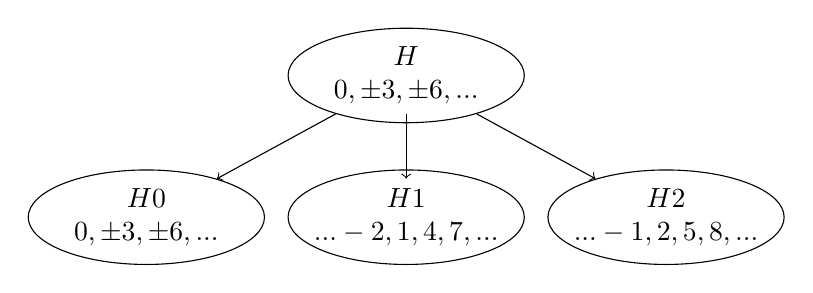
\begin{tikzpicture}[scale=0.6]
\draw (0, 3) circle[x radius=2.5cm, y radius=1cm] node[align=center] (H) {$H$ \\ $0, \pm 3, \pm 6, ...$}
      (-5.5, 0) circle[x radius=2.5cm, y radius=1cm] node[align=center] (H0) {$H0$ \\ $0, \pm 3, \pm 6, ...$}
      (0, 0) circle[x radius=2.5cm, y radius=1cm] node[align=center] (H1) {$H1$ \\ $... -2, 1, 4, 7, ...$}
      (5.5, 0) circle[x radius=2.5cm, y radius=1cm] node[align=center] (H2) {$H2$ \\ $... -1, 2, 5, 8, ...$};
\draw[->] (H) edge (H0)
          (H) edge (H1)
          (H) edge (H2);
\end{tikzpicture}
\caption{右陪集。整数加群的子群$H$包含所有3的倍数,用0、1、2分别加所有3的倍数可以得到三个互不相交子集。它们恰好是整数的一个分类。}
\label{fig:right-cosets-Z3}
\end{figure}

如图\ref{fig:right-cosets-Z3}所示,令$Z$为整数加群,$H$为所有3的倍数$0, \pm 3, \pm 6, ...$,它在加法下构成一个子群。我们用$Z$中的元素0从右侧加\footnote{由于整数加群是阿贝尔群,加法满足交换律,所以左右陪集相同。}$H$中的每个元素得到$H0$,显然这一结果还等于$H$,是所有模3余0的整数,记为[0];用$Z$中的元素1从右侧加$H$中的每个元素得到$H1$,它包含所有模3余1的整数,记为[1];用$Z$中的元素2从右侧加$H$中的每个元素得到$H2$,它包含所有模3余2的整数,记为[2]。如果用3加所有$H$的元素,结果和$H0$一样。事实上,如果我们用$H0$中的任何元素$a$获得的右陪集$Ha$都等于$H0$;用$H1$中的任何元素$b$获得的右陪集$Hb$都等于$H1$,用$H2$中的任何元素$c$获得的右陪集$Hc$都等于$H2$。$H0$、$H1$、$H2$三个右陪集放在一起恰好是全体整数$Z$。它们的确是$Z$的一个分类:[0], [1], [2]。

%% \begin{figure}[htbp]
%% \centering
%% \begin{tikzpicture}[scale=0.6]
%% \draw (0, 3) circle[x radius=2.5cm, y radius=1cm] node[align=center] (H) {$H$ \\ $(1), (1\ 2)$}
%%       (-5.5, 0) circle[x radius=2.5cm, y radius=1cm] node[align=center] (H1) {$H(1)$ \\ $(1), (1\ 2)$}
%%       (0, 0) circle[x radius=2.5cm, y radius=1cm] node[align=center] (H13) {$H(1\ 3)$ \\ $(1\ 3), (1\ 2\ 3)$}
%%       (5.5, 0) circle[x radius=2.5cm, y radius=1cm] node[align=center] (H23) {$H(2\ 3)$ \\ $(2\ 3), (1\ 3\ 2)$};
%% \draw[->] (H) edge (H1)
%%           (H) edge (H13)
%%           (H) edge (H23);
%% \end{tikzpicture}
%% \caption{有限非阿贝尔群的右陪集。}
%% \label{fig:right-cosets-S3}
%% \end{figure}

我们再看一个有限非阿贝尔群的例子。考虑置换群$S_3$

$S_3 = \{(1), (1\ 2), (1\ 3), (2\ 3), (1\ 2\ 3), (1\ 3\ 2)\}$,

它的子群$C_{2a} = \{(1), (1\ 2)\}$本质上和二阶循环群同构。我们用单位元恒等置换$(1)$,和另外两个置换$(1\ 3)$、$(2\ 3)$右乘$C_{2a}$得到3个右陪集:

\[
\begin{array}{rcl}
C_{2a} (1) & = & \{(1), (1\ 2)\} \\
C_{2a} (1\ 3) & = & \{(1\ 3), (1\ 2\ 3)\} \\
C_{2a} (2\ 3) & = & \{(2\ 3), (1\ 3\ 2)\}
\end{array}
\]

我们也可以用另外三个元来作右陪集:$C_{2a} (1\ 2)$、$C_{2a} (1\ 2\ 3)$、$C_{2a} (1\ 3\ 2)$。同样由于
$(1\ 2) \in C_{2a} (1)$、$(1\ 2\ 3) \in C_{2a} (1\ 3)$、$(1\ 3\ 2) \in C_{2a} (2\ 3)$,所以一定有

\[
\begin{array}{l}
C_{2a} (1) = C_{2a} (1\ 2) \\
C_{2a} (1\ 3) = C_{2a} (1\ 2\ 3) \\
C_{2a} (2\ 3) = C_{2a} (1\ 3\ 2)
\end{array}
\]

这样,子群$C_{2a}$把整个群$G = S_3$分成$C_{2a} (1)$、$ C_{2a} (1\ 3)$、$C_{2a} (2\ 3)$三个不同的右陪集,这三个右陪集放在一起正是$G$,它们是$G$的一个分类。

\index{左陪集}
与右陪集对称,我们也可以定义左陪集。规定对称的等价关系$\sim'$:

\[
a \sim' b \text{当且仅当} b^{-1}a \in H
\]

这样,由等价关系$\sim'$所决定的类叫做子群$H$的左陪集。包含元素$a$的左陪集用符号$aH$来表示。它包含所有形如:$ah, h \in H$形式的$G$的元。因为一个群的乘法不一定满足交换律,所以一般来说$\sim$和$\sim'$两个等价关系并不相同,$H$的左右陪集也不相同。但是一个子群的左右陪集之间有一个共同点:

\begin{theorem}
子群$H$的左右陪集个数相等,他们或者都是无限大,或者都有限并相等。
\end{theorem}

要想证明这一点,我们可以构造一个从$H$的右陪集到左陪集间的映射:$f: Ha \to a^{-1}H$。容易验证,这是一个一一映射。任意$Ha = Hb$,都有$ab^{-1} \in H$,所以$(ab^{-1})^{-1} = ba^{-1} \in H$。因此$a^{-1}H= b^{-1}H$。既然一一映射存在,自然左右陪集的个数是相等的。

\index{子群的指数}
为此,我们可以将子群$H$的陪集个数(左或者右)定义为$H$在$G$中的\textbf{指数}。

上述$S_3$的例子中,我们用了子群$C_{2a} = \{(1), (1\ 2)\}$作为等价关系,实现了对$S_3$中元素的分类。$S_3$还有另外一个子群$C_3 = \{(1), (1\ 2\ 3), (1\ 3\ 2)\}$,即三阶循环群。我们也可以用它作为等价关系对$S_3$中的置换进行分类。

\[
\begin{array}{l}
C_3 (1) = C_3 \\
C_3 (1\ 2) = \{(1\ 2), (1\ 3), (2\ 3)\}
\end{array}
\]

这两种不同的分类如图\ref{fig:S3-Cayley}和\ref{fig:S3-Cayley-aH}所示。它们存在一个重要的不同点。子群$C_3$产生的左右陪集是相同的,而$C_{2a}$产生的左右陪集是不同的。

\begin{figure}[htbp]
 \centering
 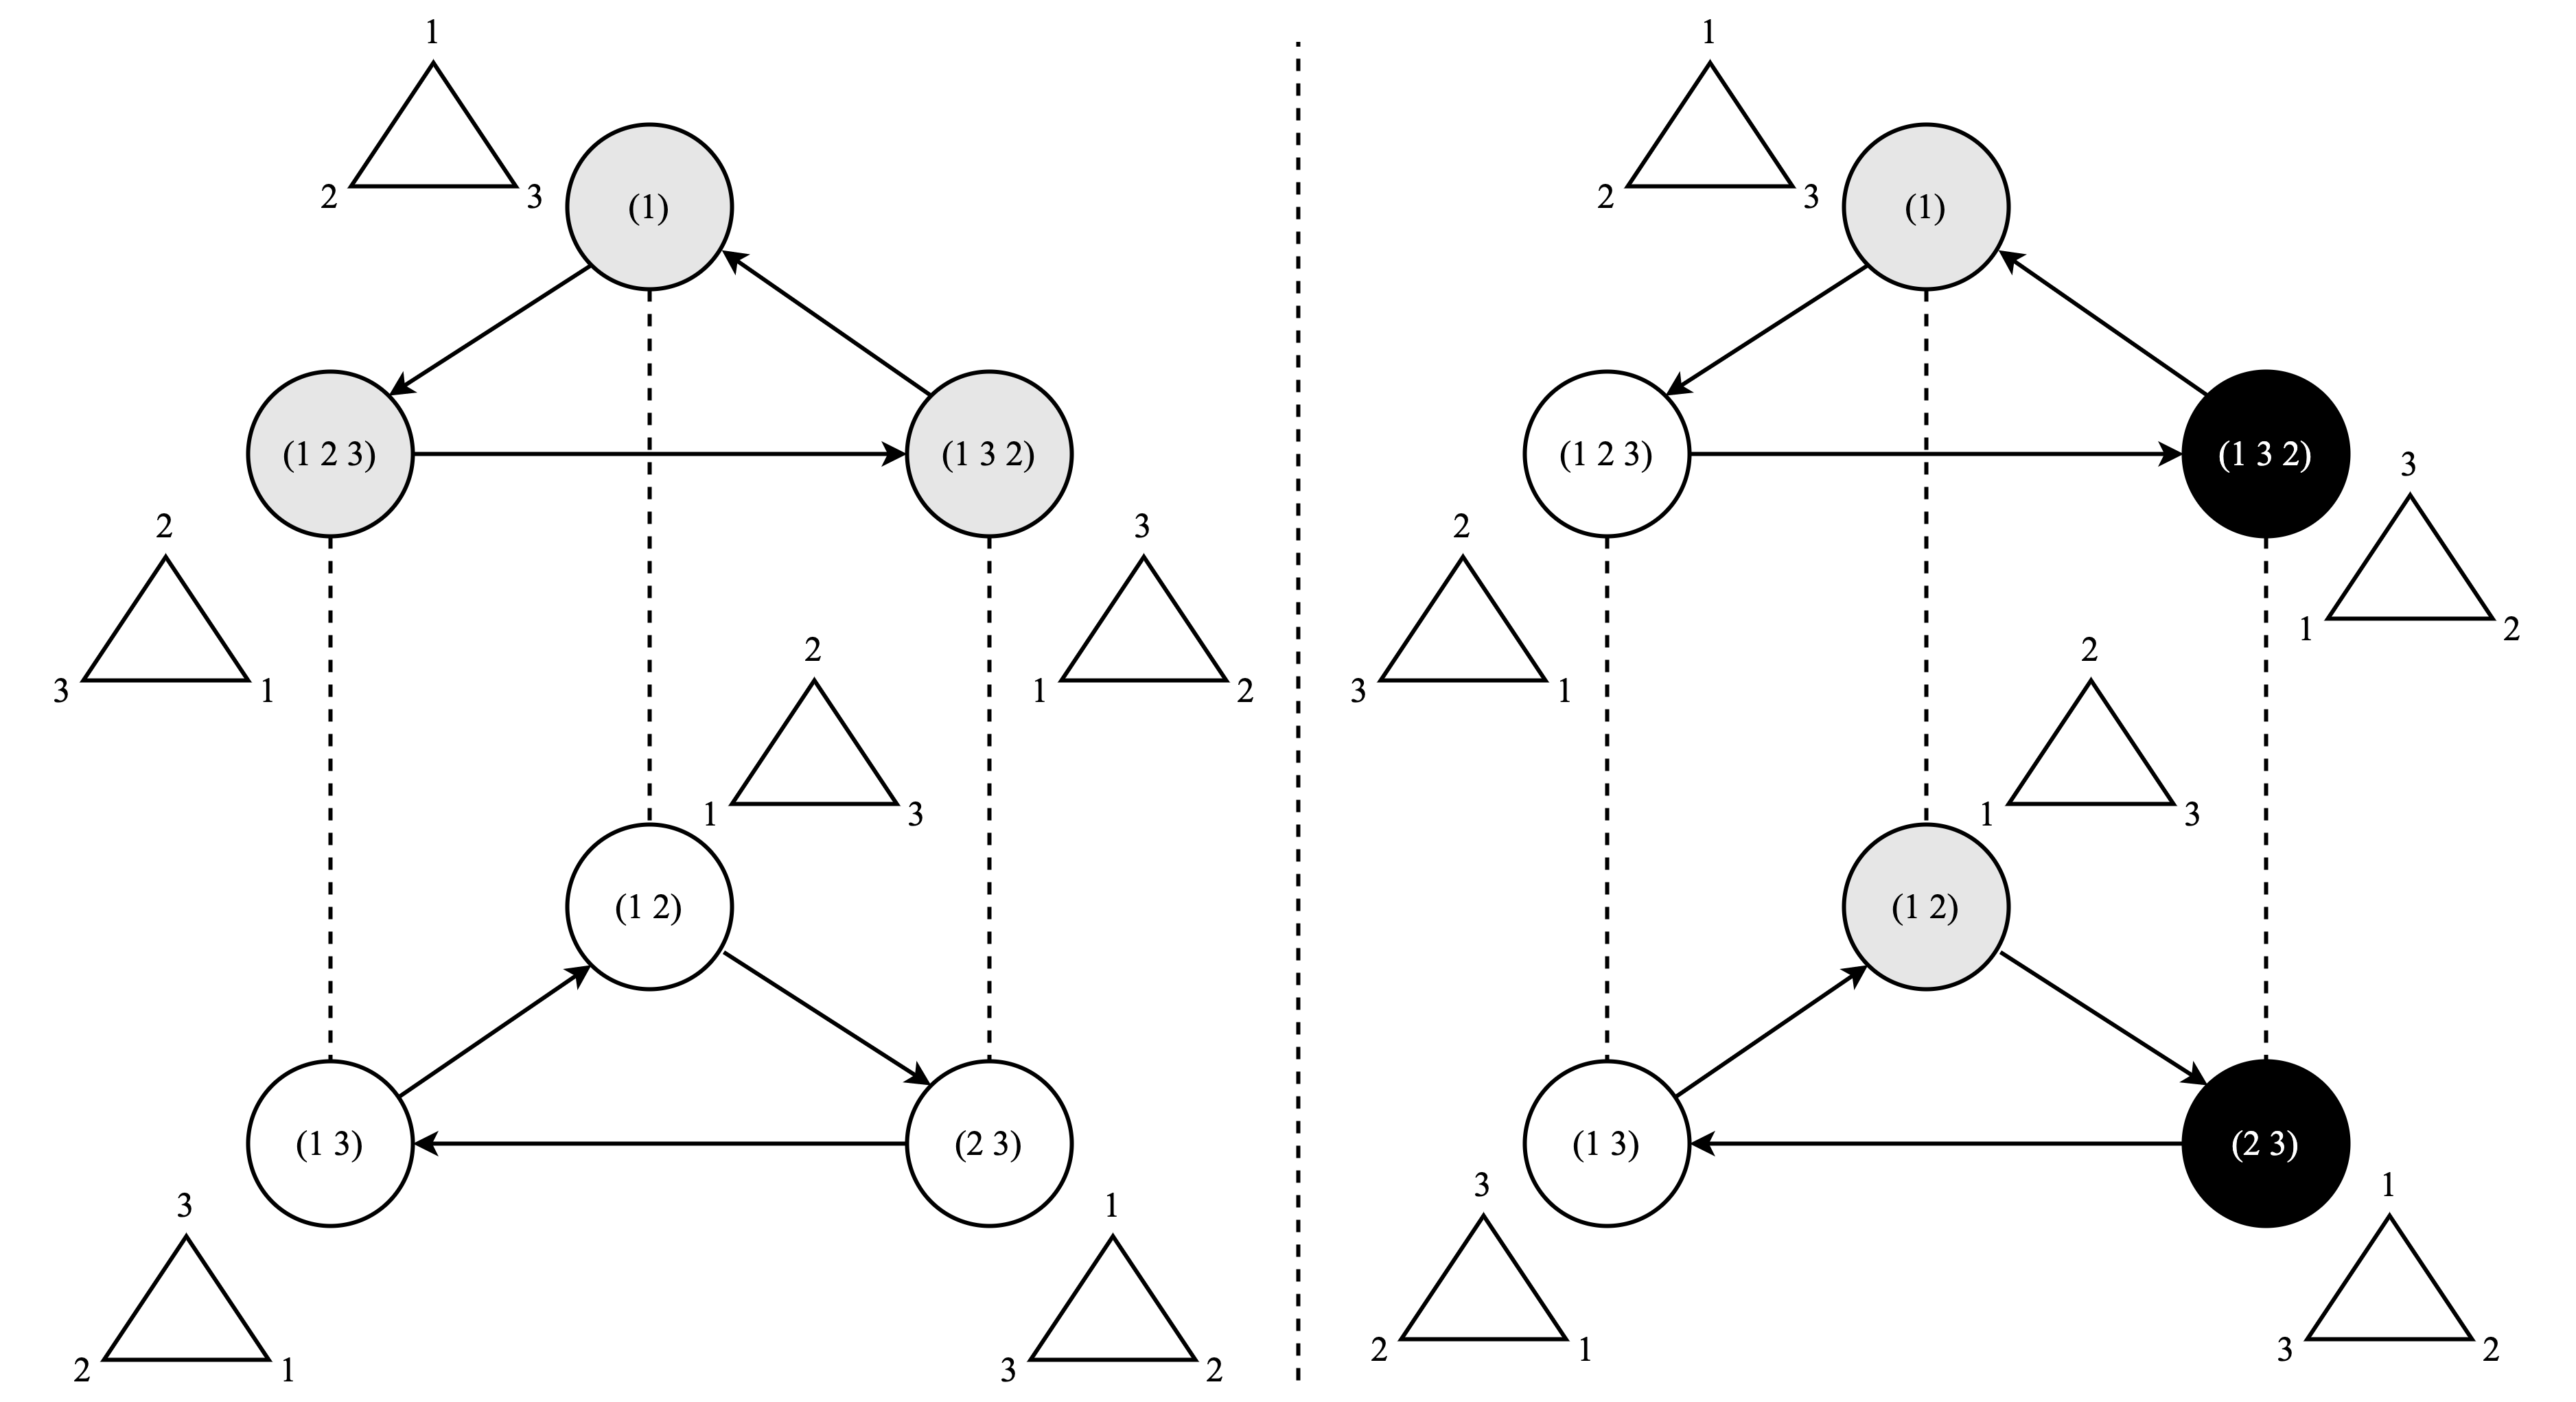
\includegraphics[scale=0.4]{img/S3-Cayley}
 \caption{用$S_3$的不同子群产生的右陪集}
 \label{fig:S3-Cayley}
\end{figure}

\btab{|c|c|c|}
\hline
子群 & $C_3$ & $C_{2a}$ \\
\hline
左陪集 & $C_3 + \{(1\ 2), (1\ 3), (2\ 3)\}$ & $C_{2a} + \{(1\ 3), (1\ 3\ 2)\} + \{(2\ 3), (1\ 2\ 3)\}$ \\
\hline
右陪集 & $C_3 + \{(1\ 2), (1\ 3), (2\ 3)\}$ & $C_{2a} + \{(1\ 3), (1\ 2\ 3)\} + \{(2\ 3), (1\ 3\ 2)\}$ \\
\hline
\etab

\begin{figure}[htbp]
 \centering
 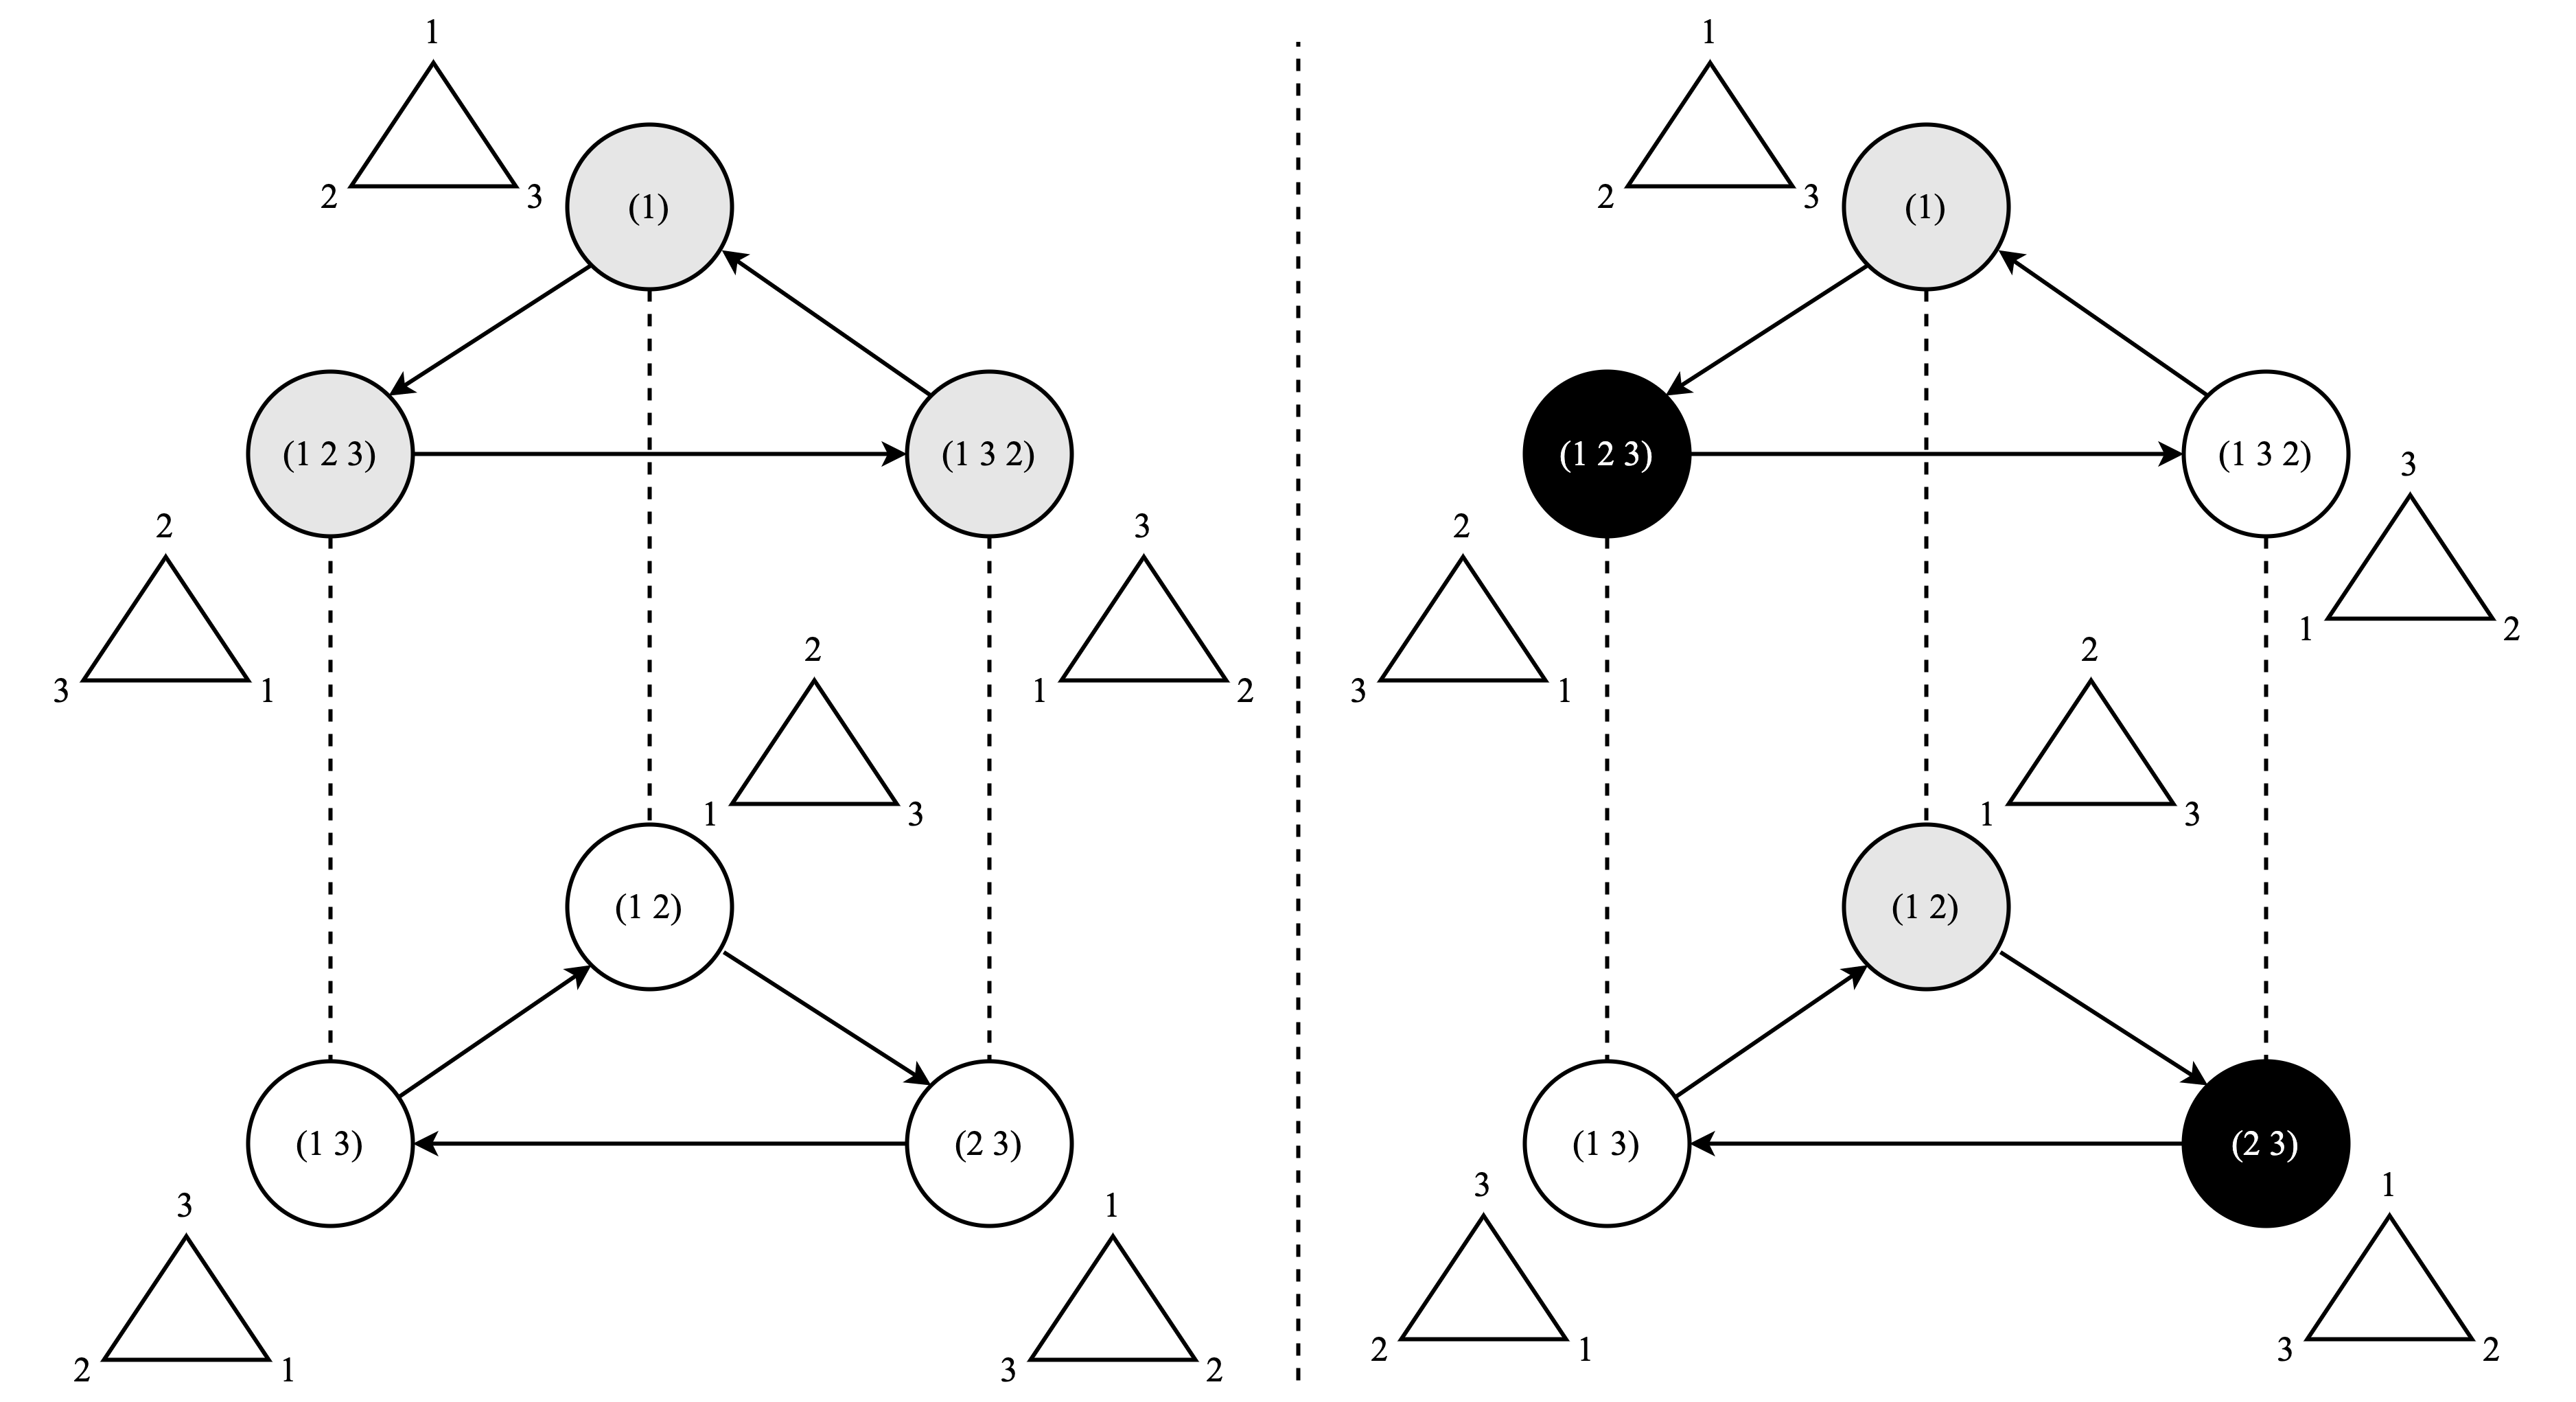
\includegraphics[scale=0.4]{img/S3-Cayley-aH}
 \caption{用$S_3$的不同子群产生的左陪集}
 \label{fig:S3-Cayley-aH}
\end{figure}

一般情况下,子群的右陪集$Ha$未必等于左陪集$aH$,如果相等,这时的子群叫做正规子群。正是伽罗瓦第一个引入了正规子群来分析方程的可解性。伽罗瓦最初称这样特殊的子群为“不变子群”,因为它使得$G$的两种分解不变:

\[
G = H a_1 + H a_2 + ... = a_1 H + a_2 H + ...
\]

\index{正规子群} \index{不变子群}
\begin{definition}
一个群$G$的子群$N$叫做一个\textbf{正规子群}(或者不变子群),假如对$G$的每个元$a$都有:
\[
Na = aN
\]
记作:$N \lhd G$或$G \rhd N$。一个正规子群的左(或右)陪集叫做$N$的\textbf{陪集}。
\label{normal-subgroup}
\end{definition}

由于其对称性,正规子集也叫做群的中心。判断一个群是否是正规子群,我们有以下两个定理:

\begin{theorem}
一个群$G$的子群$N$是一个不变子群的充分必要条件是对$G$中的任何一个元$a$都有:
\[
aNa^{-1} = N
\]
\end{theorem}

\begin{theorem}
一个群$G$的子群$N$是一个不变子群的充分必要条件是对$G$中的任何一个元$a$,$N$中的任何一个元$n$都有:
\[
ana^{-1} \in N
\]
\end{theorem}

我们可以把正规子群$N$的所有陪集做成一个集合$\{aN, bN, cN, ...\}$,并且定义这个集合上的乘法为:

\[
(xN)(yN) = (xy)N
\]

\index{商群}
可以验证,正规子群的陪集在这个乘法下构成一个群,叫做\textbf{商群},用$G/N$表示。在正规子群、商群和同态映射之间存在着重要的关系。首先一个群$G$同它的每个商群$G/N$同态。要证明这一点,我们可以构造一个映射$a \to aN, a \in G$。这显然是一个从$G$到商群的满射,对于$G$中任何两个元素$a, b$,都有$ab \to abN = (aN)(bN)$。所以它是一个同态满射。这样我们既可以通过正规子群,也可以通过商群推测群$G$的性质。为了做到这一点,我们定义一下“核”的概念。

\index{核}
\begin{definition}
若$f$是群$G$到另一个群$G'$的同态满射,$G'$的单位元$e'$在映射$f$之下的逆像集合是$G$中的一个子集。这个子集叫做同态满射$f$的\textbf{核}。
\end{definition}

我们有如下定理,如果$G$和$G'$同态,那么这个同态满射的核$N$是$G$的正规子群。并且其商群$G/N \cong G'$。这样一个群不仅和和它的每一个商群同态,并且抽象地来看,$G$只能和它的商群同态。有时候,我们发现群$G$和$G'$同态,但是$G'$的性质我们并不清楚,这时候,我们一定能找到$G$的一个正规子群$N$,使得$G'$的性质和商群$G/N$完全一样。从这里我们能看出不变子群和商群的意义。伽罗瓦正是通过这一点,想出并定义了方程的群的可解性。

\begin{Exercise}
\Question{证明子群的判定定理\ref{theorem:subgroup}。}
%\Question{列出图\ref{fig:right-cosets-S3}中$H$的左陪集。}
\end{Exercise}

\subsection{拉格朗日定理}
\index{拉格朗日}

拉格朗日定理是特别体现抽象代数特点的一个定理。在完全无须了解群中元素和运算的具体意义的情况下,我们仍可以揭示抽象结构的内在规律。

%\begin{figure}[htbp]
\begin{wrapfigure}{R}{0.4\textwidth}
 %\raggedright
 \centering
 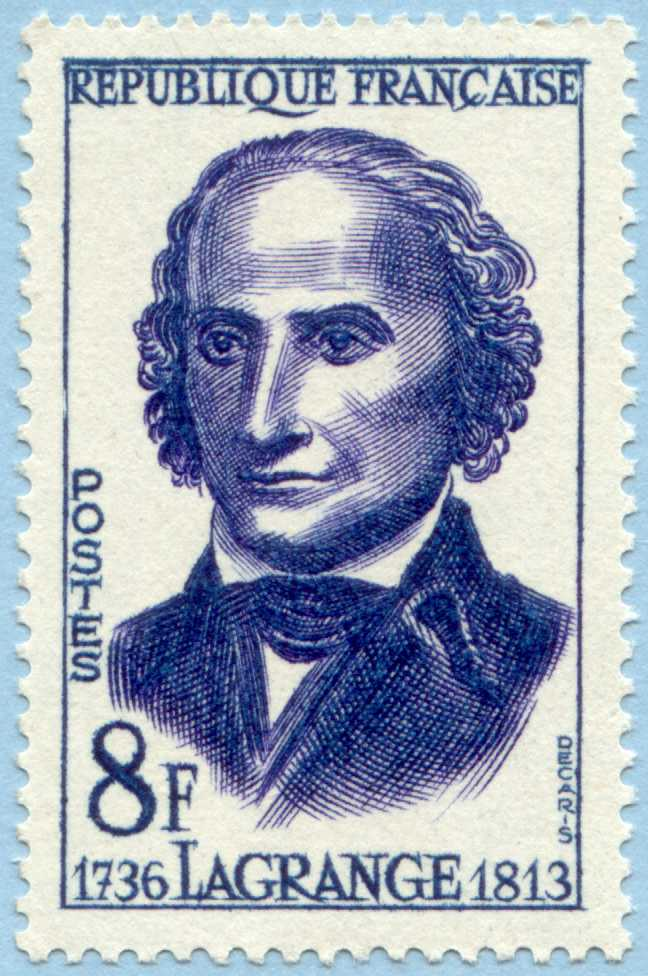
\includegraphics[scale=1.5]{img/lagrange.jpg}
 \captionsetup{labelformat=empty}
 \caption{拉格朗日纪念邮票}
 \label{fig:Lagrange}
\end{wrapfigure}
%\end{figure}

% 拉格朗日(Joseph-Louise Lagrange)
拉格朗日全名为约瑟夫$\cdot$路易斯$\cdot$拉格朗日,是著名数学家、物理学家。1736年1月25日生于意大利都灵。拉格朗日的祖先是法国军官,到意大利后与罗马家族的人结婚定居。他的父亲曾任都灵的公共事务和防务局会计,但后来由于经商破产,家道中落。据拉格朗日本人回忆,如果幼年时家境富裕,他也就不会作数学研究了,因为父亲一心想把他培养成为一名律师。拉格朗日在都灵大学读书时,并没有对数学发生兴趣,他觉得欧几里得几何很枯燥。

17岁时,拉格朗日碰巧看到了英国天文学家哈雷的一篇介绍牛顿微积分的文章。他一下子被吸引住了。开始全身心投入学习数学。1755年拉格朗日19岁时,在探讨数学难题“等周问题”的过程中,他以欧拉的思路和结果为依据,用纯分析的方法求变分极值。第一篇论文“极大和极小的方法研究”,发展了欧拉所开创的变分法,为变分法奠定了理论基础。变分法的创立,使拉格朗日在都灵声名大振,并使他在19岁时就当上了都灵皇家炮兵学校的教授,成为当时欧洲公认的第一流数学家。1756年,受欧拉的举荐,拉格朗日被任命为普鲁士科学院通讯院士。

1766年德国的腓特烈大帝向拉格朗日发出邀请时说,在“欧洲最大的王”的宫廷中应有“欧洲最大的数学家”。于是他应邀前往柏林,任普鲁士科学院数学部主任,居住达20年之久,开始了他一生科学研究的鼎盛时期。在此期间,他完成了《分析力学》一书,这是牛顿之后的一部重要的经典力学著作。书中运用变分原理和分析的方法,建立起完整和谐的力学体系,使力学分析化了。

腓特烈大帝非常欣赏拉格朗日,常常和他谈论规律生活的重要性。在皇帝的影响下,拉格朗日每天晚上都想好明天要完成的具体任务。每当工作取得进展,他都写一段简短的分析看看哪里还能进一步改进。拉格朗日在撰写论文前总是深思熟虑,他通常能一气呵成而不用修改。但拉格朗日不太习惯柏林的气候,他的身体一直不太好。1783年,他的妻子维多利亚因病去世。

1786年一直支持他的腓特烈大帝也去世了。拉格朗日接受了路易十六的邀请来到巴黎。他得到了特别的接待,国王甚至在卢浮宫里为他安排了一处住所。1792年,拉格朗日的朋友,天文学家勒莫尼埃(LeMonnier)的女儿,24岁蕾妮(Renée Francoise Adelaide)坚持要嫁给孤单一人的拉格朗日。他们结婚后虽未生儿女,但家庭幸福。

这时法国大革命爆发了。1793年9月革命政府决定逮捕所有在敌国出生的人,著名化学家拉瓦锡在身处危险的情况下竭力奔走相助,终于才把拉格朗日作为例外。1794年5月4日法国雅各宾派开庭审判波旁王朝税务人员,把包括拉瓦锡在内的28名成员全部处以死刑。拉格朗日等人尽力地挽救,请求赦免,但是遭到了革命法庭副长官考费那尔(J.B.Coffinhal)的拒绝,全部予以驳回,并宣称,“共和国不需要学者,而只需要为国家而采取的正义行动!”5月8日早晨,拉格朗日痛心地说:“他们可以一眨眼就把拉瓦锡的头砍下来,但他那样的头脑一百年也再长不出一个来了。”\cite{Wiki-Lagrange}

1799年雾月政变后,拿破仑热情支持法国的科学研究。他提名拉格朗日等著名科学家成为上议院议员及新设的勋级会荣誉军团成员,封为伯爵;还在1813年4月3日授予他帝国大十字勋章。此时拉格朗日已重病在身,终于在4月11日晨逝世。在葬礼上,由议长拉普拉斯代表上议院,院长拉赛佩德(Lacépède)代表法兰西研究院致悼词。意大利各大学都举行了纪念活动。

拉格朗日是18世纪的伟大科学家,在数学、力学和天文学三个学科中都有历史性的重大贡献。但他主要是数学家,拿破仑曾称赞他是“一座高耸在数学界的金字塔”,他最突出的贡献是在把数学分析的基础脱离几何与力学方面起了决定性的作用。使数学的独立性更为清楚,而不仅是其它学科的工具。同时在使天文学力学化、力学分析化上也起了历史性作用,促使力学和天文学(天体力学)更深入发展。

拉格朗日在柏林的前十年,把大量时间花在代数方程和超越方程的解法上。他在代数方程解法中有历史性贡献。他把前人解三、四次代数方程的各种解法,总结为一套标准方法,而且还分析出一般三、四次方程能用代数方法解出的原因。三次方程有一个二次辅助方程,其解为三次方程根的函数,在根的置换下只有两个值;四次方程的辅助方程的解则在根的置换下只有三个不同值,因而辅助方程为三次方程。拉格朗日称辅助方程的解为原方程根的预解函数(是有理函数)。他继续寻找5次方程的预解函数,希望这个函数是低于5次的方程的解,但没有成功。尽管如此,拉格朗日的想法已蕴含着置换群概念,而且使预解(有理)函数值不变的置换构成子群,子群的阶是原置换群阶的因子。这正是群论中著名的拉格朗日定理。拉格朗日是群论的先驱。他的思想为后来的阿贝尔和伽罗瓦采用并发展,终于解决了五次以上的一般方程为何不能用代数方法求解的问题。

在介绍拉格朗日定理前,我们首先看一个引理:

\begin{lemma}
一个子群$H$与其每一个右陪集$Ha$之间都存在一一映射。
\end{lemma}

由于陪集的左右对称性,这一结论对于左陪集也成立。要想证明它,我们可以构造映射$f: h \to ha$,它就是一个从子群到右陪集的一一映射,因为:

\begin{enumerate}
\item $H$中的每个元素$h$都有一个唯一的像$ha$;
\item $Ha$中的每个元素$ha$都是子群$H$中元素$h$的像;
\item 任意$h_1a = h_2a$,都有$h_1 = h_2$。
\end{enumerate}

由于一一映射的存在,我们知道有限群$G$中,陪集中元素的个数一定与子群$H$的阶相等。而且由于陪集的分类特性,我们知道群中的每个元素都可以在某一个陪集中找到。这样我们就可以利用陪集发现子群$H$与有限群$G$之间的一个关系:

\index{拉格朗日定理}
\begin{theorem}
\textbf{拉格朗日定理}:有限群$G$的阶,能够被其子群$H$的阶整除。
\end{theorem}

\begin{proof}
首先,我们知道$G$能够为$H$的陪集全部覆盖;并且由于陪集之上定义的等价关系,我们知道陪集之间是没有交集的。如果存在元素$c$既属于$Ha$,也属于$Hb$,那么$c \sim a$,$c \sim b$,所以$a \sim b$,所以$Ha = Hb$。再加上子群$H$与陪集存在一一映射的引理,我们知道每个陪集的大小都等于$H$的阶$|H|=n$,如果陪集的个数(也就是$H$的指数)等于$m$,一定有
\[
|G| = mn
\]
\end{proof}

注意,拉格朗日定理的逆定理不一定成立。我们无法将群的阶做任意因子分解,然后对每个因子都找到子群和陪集。我们在本章结尾的图\ref{fig:group-graph}(c)中会看到这样一个反例。交错群$A_4$含有12个元素,但是却没有阶为6的子群。从拉格朗日定理,我们可以得到很多有用的推论。

\begin{corollary}
一个有限群$G$中的任意元素$a$的阶都能整除$G$的阶。
\end{corollary}

这是因为$a$生成一个阶为$n$的子群,所以$n$能整除$|G|$。

\begin{corollary}
如果$G$的阶是素数,那么$G$是循环群。
\end{corollary}

这是因为任何不等于单位元的元素$a$,它所生成的子群的阶一定等于$G$的阶。所以$a$是$G$的生成元,即$G = (a)$。

\begin{corollary}
有限群$G$中的任何元素$a$,都有$a^{|G|} = e$。
\label{corollary:Lagrange-elem-order}
\end{corollary}

这是因为$a$的阶$n$能够整除$G$,不妨令$|G| = nk$。所以
\[
a^{|G|} = a^{nk} = (a^n)^k = e^k = e
\]

群论中的拉格朗日定理可以用来证明数论中著名的费马小定理和欧拉定理。费马小定理是法国数学家费马于1636年发现的。他在1640年10月18日写给友人\footnote{费马的朋友法国数学家贝西(Bernard Frénicle de Bessy)}的信中首次提出了这个定理。1736年,欧拉给出了费马小定理的一个证明。但从莱布尼茨未发表的手稿中发现他在1683年以前已经得到几乎相同的证明。之所以命名为“小定理”是为了区别于举世闻名的费马大定理。

\index{费马小定理}
\begin{theorem}
\textbf{费马小定理}:若$p$是素数,对任何满足$0 < a < p$的整数$a$都有,$a^{p-1}-1$能被$p$整除。
\end{theorem}

\begin{proof}
考虑整数模$p$乘法群。这个群的元素由所有模$p$的非零余数构成,因为$p$是素数,所以群元素为1, 2, ..., $p-1$,单位元$e = 1$,群的阶为$p-1$。根据拉格朗日定理的推论\ref{corollary:Lagrange-elem-order},有:
\[
a^{p-1} = e
\]
因为单位元为1,所以上式可写为:
\[
a^{p-1} \equiv 1 \mod p
\]
故$p$整除$a^{p-1} - 1$。
\end{proof}

和这一证明对比,初等数论方法的证明要复杂得多(\cite{StepanovRose15}第5.2到5.4)。我们再介绍另一种有趣的“项链”证法\cite{Wiki-FLT-proof},供读者参考。

\begin{proof}
考虑有$a$种不同颜色的珍珠,我们要串一条长为$p$的珍珠串。其中$p$为素数。显然一共有$a^p$种不同的串,这是因为串中每个位置都可以在$a$种颜色的珍珠中选择,共选$p$次。

例如有两种颜色$A$红、$B$绿的珍珠,要串长度为5的串。即$a = 2, p = 5$,一共有$2^5 = 32$种不同的串:

\begin{verbatim}
  AAAAA, AAAAB, AAABA, ..., BBBBA, BBBBB.
\end{verbatim}

对应:红红红红红, 红红红红绿, 红红红绿红, ..., 绿绿绿绿红, 绿绿绿绿绿.

我们要证明,在这$a^p$串珍珠中,如果去掉$a$个颜色完全相同的串(在上述例子中是串\texttt{AAAAA}和\texttt{BBBBB}),剩下的$a^p - a$串珍珠可以分成若干组,每个组恰好有$p$串珍珠。也就是说$p$整除$a^p - a$。

如果把每串珍珠首尾连接起来做成项链。原来有些不同的串会变成相同的项链。如果一个串可以通过旋转变换成另一个,这两个串必然做成相同的项链。例如下面的5串珍珠可以做成相同的项链:

\begin{verbatim}
  AAAAB, AAABA, AABAA, ABAAA, BAAAA.
\end{verbatim}

\begin{figure}[htbp]
  \centering
  \subcaptionbox{一串含3种颜色的项链代表7种不同的串:\texttt{ABCBAAC}, \texttt{BCBAACA}, \texttt{CBAACAB}, \texttt{BAACABC}, \texttt{AACABCB}, \texttt{ACABCBA}, \texttt{CABCBAA}}[0.45\linewidth]{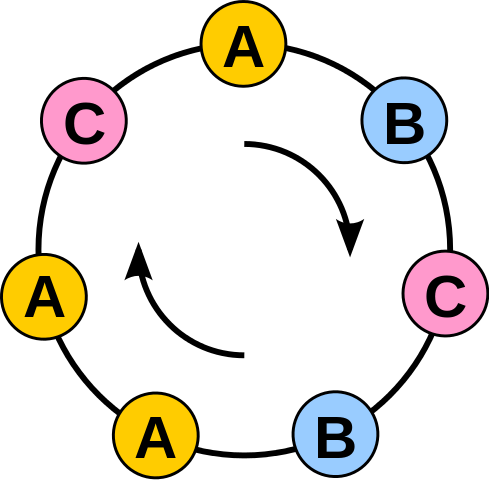
\includegraphics[scale=0.2]{img/bracelet-rotate.png}} \quad
  \subcaptionbox{相同颜色珍珠串成的项链只代表一种串:\texttt{AAAAAAA}}[0.45\linewidth]{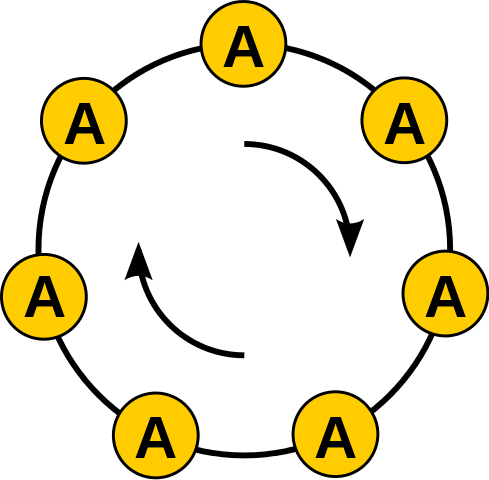
\includegraphics[scale=0.2]{img/bracelet-identical.png}}
  \caption{通过项链对珍珠串进行分类}
  \label{fig:bracelet}
\end{figure}

用这种方法,上面例子中的32串珍珠可以分成5种不同颜色的项链和2种同色的项链:

\begin{verbatim}
  [AAABB, AABBA, ABBAA, BBAAA, BAAAB];
  [AABAB, ABABA, BABAA, ABAAB, BAABA];
  [AABBB, ABBBA, BBBAA, BBAAB, BAABB];
  [ABABB, BABBA, ABBAB, BBABA, BABAB];
  [ABBBB, BBBBA, BBBAB, BBABB, BABBB];
  [AAAAA];
  [BBBBB].
\end{verbatim}

一串项链可以代表多少种不同的串呢?如果一个串$S$由若干相同的子串$T$复制连接而成,而$T$无法再继续分拆成相同的子串,则由$S$构成的项链可代表$|T|$种不同的串,其中$|T|$表示串$T$的长度。例如串$S=$\texttt{ABBABBABBABB},由相同的子串$T=$\texttt{ABB}复制多次而成,如果我们一次旋转一颗珍珠,一共可以得到3串不同的结果:

\begin{verbatim}
  ABBABBABBABB,
  BBABBABBABBA,
  BABBABBABBAB.
\end{verbatim}

除去这3种之外,不可能再有其它不同种类的串了。\texttt{ABB}的长度为3,再次旋转必然会循环得到相同的结果。这样,所有的$a^p$串珍珠可分成两类。一类是$a$串颜色相同的串;另一类颜色不同,但是由于这些串的长度$p$是素数,它绝不可能由若干子串复制连接出来。所以任何一个这样的串连成的项链,总共代表$p$种不同的串。而这样的串总共有$a^p - a$种,它们可以通过连成项链后分组,每组恰好$p$个串,代表一种不同的项链。因此$a^p-a = a(a^{p-1}-1)$一定可以被$p$整除。由于$a$和$p$互素,所以$p$一定整除$a^{p-1}-1$。
\end{proof}

项链证明法可能是费马小定理已知证法中最容易的,它不需要太多的数学知识。核心思想是利用两种不同的方式数数的结果必然是一样的。

%\begin{figure}[htbp]
\begin{wrapfigure}{L}{0.35\textwidth}
  \centering %\raggedleft
 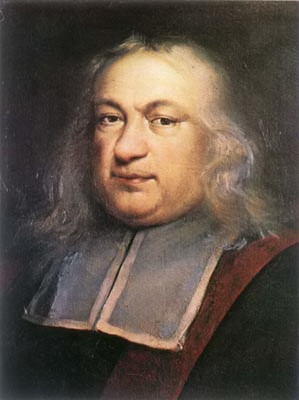
\includegraphics[scale=0.4]{img/Fermat.jpg}
 \captionsetup{labelformat=empty}
 \caption{皮埃尔$\cdot$德$\cdot$费马 1601-1665}
 \label{fig:Fermat}
\end{wrapfigure}
%\end{figure}

费马小定理从提出到欧拉成功证明经过了整整100年。这是费马的一贯风格,费马大定理(也称费马的最后定理)难住了无数天才数学家,历经358年才由英国数学家安德鲁$\cdot$怀尔斯在1995年成功攻克。而怀尔斯的主要武器包括椭圆曲线、模形式和伽罗瓦表示\cite{HanXueTao2009}。可以说费马留下的这些猜想是一笔丰富的数学遗产。

\vspace{5mm}

\index{费马(Pierre de Fermat )}
费马是法国著名数学家,1601年8月生于法国图卢兹一个富有的皮革商人家中。他是一位全职律师,一直在司法部门工作,后来还当过图卢兹最高法院的大法官。费马在成年后才开始利用业余时间研究数学。但费马取得的数学成就,堪称那个时代的高峰。1629年,费马独立得到了解析几何的基本原理\footnote{费马的8页论文《平面与立体轨迹引论》在1630年完成,但在1679年费马死后14年才出版。},因而与笛卡尔分享创立解析几何的荣誉;他与帕斯卡在一段漫长而有趣的通信中一起奠定了古典概率论的基础,提出了数学期望的概念,因而与帕斯卡被公认为是概率论的创始人;他提出光学中的“费马原理”\footnote{又称最小作用原理,或最短时间作用原理。},给后来变分法的研究以极大的启示;他是创建微积分学的杰出先驱者。而费马本人最感兴趣的领域是数论。

费马对数论的兴趣是由古希腊数学家丢番图的名著《算术》启发的。1621年,巴谢(Bachet)校订注释的希腊——拉丁文对照本在法国出版。费马在巴黎买到此书,并被其中的数论问题深深吸引。值得庆幸的是,这一版的每一页都留有宽大的空白页边,于是这书同时成了费马的笔记本。在研究丢番图的问题和解答时,他会受到启发去思考和解决更多、更深入的问题,并草草地在这些空白书边上写下自己的评注。

费马在其生前,几乎没有公开发表过任何他的数学成果。这在“不发表就发霉”的今天是很难被理解的。除了把自己的研究成果写在书籍的页边,费马也常常按照当时流行的风气,以书信的形式向一些学者朋友报告。究其原因,费马是被“发现新的数学奥秘”这类强烈的念头所驱使的。研究数学对于他是一种消遣,纯粹是由于他对数学的爱好。当创造出他从未触及的结果时,费马会获得真正的愉悦与自我满足。因而公开发表和被人们承认对他而言没有多大意义\cite{HanXueTao2009}。有趣的是,这位缄默的天才有时喜好捉弄人,他经常在信中向其他数学家发出挑战,要求他们证明自己发现的某些数学结果。

\begin{wrapfigure}{R}{0.33\textwidth}
%\begin{figure}[htbp]
 \centering
 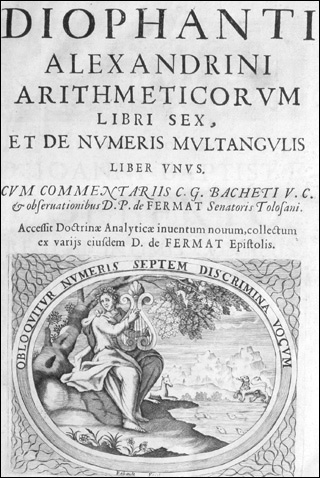
\includegraphics[scale=0.4]{img/Arithmetica.jpg}
 \captionsetup{labelformat=empty}
 \caption{丢番图《算术》1670年版,带有费马评注}
 \label{fig:Arithmetica}
%\end{figure}
\end{wrapfigure}

当费马在1665年1月去世时,他的研究成果散落各处。费马的长子塞缪尔(Samuel)花了5年时间整理信件收集注记,1670年将他父亲的成果出版为一个特殊版本的《算术》。在封面图片上方,写着“附有费马的评注”的小字。这一版本包括费马所做的48个评注。1679年,他又整理了出版了费马的第二卷著作。费马生前的这些研究成果终于得以流传,极大地丰富了十七世纪的数学宝库,推动了后来的数学发展。

在费马之前,数论基本上是一些相关问题的汇集。费马振兴了数论的研究,系统地提出了数量众多的数论定理,并引入了一般化的方法和原理,从而把数论引上了近代发展的轨道。可以说,正是费马的系统化工作,数论才真正开始成为一门数学分支。费马也因此奠定近代数论的基础,而被称为“近代数论之父”。在高斯的《算术研究》出版之前,数论的发展始终是跟费马的推动联系在一起的。

然而,费马生前提出的种种结论常常仅含有证明的一些关键部分,有时甚至根本没有证明。有些内容后来发现是错误的\footnote{例如费马数。费马在1640年宣称$2^{2^n}+1$形式的数都是素数,并且当$n$为0, 1, 2, 3, 4时都是对的。它们分别是3, 5, 17, 257, 65537。但欧拉在1732年算出$2^{2^5} + 1 = 641 \times 6700417$。目前(2017年)人们已经找到243个反例,却没有再发现第6个费马素数。是否还有其它费马素数至今没有人能够解决。}。因此在找到严格的数学证明前,这些结论只能称之为“猜想”。这些猜想有很多是被欧拉攻克的,不仅如此,欧拉还在费马的基础上发展了更多的结果。

我们接下来要介绍的数论中的欧拉定理,就是比费马小定理更加普遍的结果。在成功证明了费马小定理后,欧拉并不满足,如果$p$不是素数会怎样呢?欧拉仔细研究了合数的情况,得出并证明了下面的定理。

\index{欧拉定理} \index{欧拉函数}
\begin{theorem}
\textbf{欧拉定理}:如果$0 < a < n$且$a$与$n$互素,那么$a^{\upphi(n)} - 1$能够被$n$整除。
\end{theorem}

其中$\upphi(n)$是欧拉函数\footnote{也称为欧拉总计函数(Euler totient function)或者欧拉$\upphi$函数},它的定义是所有小于$n$且与$n$互素的正整数个数。即:

\[
\upphi(n) = |\{i | 0 < i < n\ \text{且}\ gcd(i, n) = 1 \}|
\]

欧拉使用初等数论的方法证明了这一定理。我们展示如何利用群论和拉格朗日定理给出一个简洁的证明。

\begin{proof}
考虑整数模$n$的非零余数。我们把模$n$乘法之下可以互逆的所有余数挑选出来。它们构成一个模$n$乘法群。按照欧拉$\upphi$函数的定义,$\upphi(n)$的值,是所有小于$n$且与$n$互素的正整数的个数。而这些正整数,恰好对应这个乘法群中的元素。所以这个群的阶就是$\upphi(n)$。根据拉格朗日定理的推论\ref{corollary:Lagrange-elem-order},有:

\[
a^{\upphi(n)} = e
\]

故而$a^{\upphi(n)} \equiv 1 \mod n$,所以$n$一定整除$a^{\upphi(n)} - 1$。
\end{proof}

我们举个例子,下表是模10的非零余数的乘法表。我们可以从表中找到单位元1,用下划线标出。然后从其所对应的行列找到模乘的两个数,加粗标出。这些数都和10互素。反之,那些不和10互素的余数所在的行列中都有0元素,而0不是群中的元。可以看到和10互素的余数恰好是群中的元素1, 3, 7, 9。

\vspace{5mm}
\begin{center}
\definecolor{Gray}{gray}{0.9}
\newcolumntype{g}{>{\columncolor{Gray}}c}
\begin{tabular}{c|g|c|g|c|c|c|g|c|g|}
  & \textbf{1} & 2 & \textbf{3} & 4 & 5 & 6 & \textbf{7} & 8 & \textbf{9} \\
\hline
\rowcolor{Gray}
\textbf{1} & \cellcolor{gray} \underline{1} & 2 & 3 & 4 & 5 & 6 & 7 & 8 & 8 \\
\hline
2 & 2 & 4 & 6 & 8 & 0 & 2 & 4 & 6 & 8 \\
\hline
\rowcolor{Gray}
\textbf{3} & 3 & 6 & 9 & 2 & 5 & 8 & \cellcolor{gray}\underline{1} & 4 & 7 \\
\hline
4 & 4 & 8 & 2 & 6 & 0 & 4 & 8 & 2 & 6 \\
\hline
5 & 5 & 0 & 5 & 0 & 5 & 0 & 5 & 0 & 5 \\
\hline
6 & 6 & 2 & 8 & 4 & 0 & 6 & 2 & 8 & 4 \\
\hline
\rowcolor{Gray}
\textbf{7} & 7 & 4 & \cellcolor{gray} \underline{1} & 8 & 5 & 2 & 9 & 6 & 3 \\
\hline
8 & 8 & 6 & 4 & 2 & 0 & 8 & 6 & 4 & 2 \\
\hline
\rowcolor{Gray}
\textbf{9} & 9 & 8 & 7 & 6 & 5 & 4 & 3 & 2 & \cellcolor{gray} \underline{1} \\
\hline
\end{tabular}
\end{center}
\vspace{5mm}

任给一个整数$n$,如何求出其欧拉函数的值呢?因为任何大于1的整数都可以写成素数幂的乘积形式,我们首先来看,对于素数$p$的$m$次幂,$\upphi(p^m)$如何计算。也就是求出从1到$p^m-1$中,有多少个数和$p^m$互素。显然我们只要把$p$的倍数这些数除去即可。这些数分别是:$p, 2p, 3p, ..., p^m - p$,我们把它们分别除以$p$,就可以得到自然数序列:$1, 2, 3, ..., p^{m-1} - 1$。显然共有$p^{m-1} - 1$个。于是素数的整数次幂的欧拉函数值为:

\begin{align*}
\upphi(p^m) &= (p^m - 1) - (p^{m-1} - 1) \\
            &= p^m - p^{m-1} \\
            &= p^m(1-\dfrac{1}{p})
\end{align*}

接下来我们考虑$n = p^uq^v$,也就是两个不同素数幂的积。我们首先从1到$n-1$中,减去$p$的所有倍数,然后再减去$q$的所有倍数,但是有些整数既是$p$的倍数,也是$q$的倍数,所以最后要把这些$pq$的倍数再加回来(组合中的容斥原理)。这样有:

\begin{align*}
\upphi(p^uq^v) &=  (n - 1) - (\dfrac{n}{p} - 1) - (\dfrac{n}{q} - 1) + (\dfrac{n}{pq} - 1) \\
          &=  n(1 - \dfrac{1}{p})(1 - \dfrac{1}{q}) \\[5pt]
          &=  p^u(1 - \dfrac{1}{p})q^v(1 - \dfrac{1}{q}) \\[5pt]
          &=  \upphi(p^u)\upphi(q^v)
\end{align*}

特别地,当指数$u$, $v$都是1的时候,我们有$\upphi(pq) = \upphi(p)\upphi(q)$。并且我们可以把这个结果推广到多个素数幂的情况,如果$n = p_1^{k_1}, p_2^{k_2}...p_m^{k_m}$,则其欧拉函数的值为:

\begin{align*}
\upphi(n) &= n(1-\dfrac{1}{p_1})(1-\dfrac{1}{p_2})...(1-\dfrac{1}{p_m}) \\[5pt]
    &= \upphi(p_1^{k_1})\upphi(p_2^{k_2})...\upphi(p_m^{k_m})
%\end{array}
\end{align*}

根据这一结论,我们可以找到快速求欧拉函数的方法,读着可以通过本节的习题实现这一算法。

\vspace{5mm}

\index{欧拉}
欧拉是伟大的瑞士数学家和自然科学家。人们一般把他与阿基米德、牛顿、高斯并列为数学史上最伟大的四位数学家。1707年4月15日欧拉出生于瑞士的巴塞尔。牧师家庭的父亲曾希望他学习神学。欧拉13岁考入巴塞尔大学神学院,主修哲学和法律。欧拉很快在数学方面表现出兴趣,每周六下午都和当时欧洲最优秀的数学家约翰$\cdot$伯努利学习数学。16岁时,欧拉取得了他的哲学硕士学位。之后,他遵从了父亲的意愿进入了神学系,并准备成为一名牧师。但最终约翰$\cdot$伯努利说服欧拉的父亲允许欧拉学习数学,并使他相信欧拉注定能成为一位伟大的数学家。

%\begin{wrapfigure}{R}{0.4\textwidth}
\begin{figure}[htbp]
 \centering
 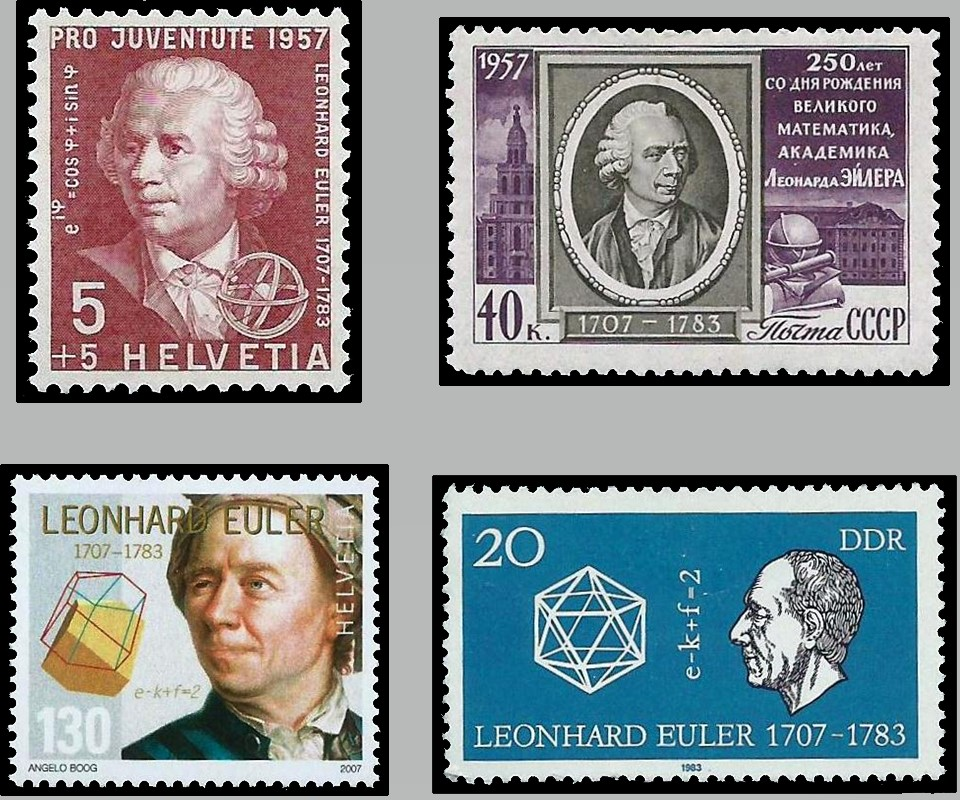
\includegraphics[scale=0.4]{img/euler.jpg}
 \captionsetup{labelformat=empty}
 \caption{各国发行的欧拉纪念邮票。欧拉(Leonhard Euler)1707 - 1783}
 \label{fig:Leonhard-Euler}
\end{figure}
%\end{wrapfigure}

1727年,欧拉成为俄罗斯圣彼得堡科学院的成员。他以旺盛的精力投入研究,在俄国的14年中,他在分析学、数论和力学方面作了大量出色的工作。1741年受腓特烈大帝的邀请到柏林科学院工作,达25年之久。在柏林期间他的研究内容更加广泛,涉及行星运动、刚体运动、热力学、弹道学、人口学,这些工作和他的数学研究相互推动。欧拉这个时期在微分方程、曲面微分几何以及其它数学领域的研究都是开创性的。1766年,叶卡捷琳娜二世在位期间,欧拉应邀重新返回圣彼得堡,并在那里直到逝世。

欧拉渊博的知识,无穷无尽的创作精力和空前丰富的著作,都是令人惊叹不已的。他从19岁开始发表论文,直到76岁,半个多世纪写下了浩如烟海的书籍和论文。几乎每一个数学领域都可以看到欧拉的名字。欧拉是科学史上最多产的一位杰出的数学家,一生发表论文共计856篇,专著31部。这还不包括1771年圣彼得堡火灾中失去的一部分。(欧拉的记录直到20世纪才由匈牙利数学家保罗·埃尔德什打破。后者发表的论文1525篇,著作32部。\cite{Wiki-Euler})

欧拉具有超出常人的坚强意志。1735年,他的右眼开始失明。1771年原本正常的左眼也完全失明了。正如失聪没有阻止贝多芬的音乐创作一样,失明也同样没有阻止欧拉的数学探索\cite{HanXueTao2009}。在书记员的帮助下,欧拉在多个领域的研究其实变得更加高产了。在1775年,他平均每周就完成一篇数学论文。欧拉一生中有一半著作都是在双目完全失明后口述完成的。欧拉的多产并不是偶然的,他有着惊人的记忆力。不但能够记住前100个素数,而且还能记住它们的平方、立方甚至更高次方。他还可以进行复杂的心算。法国物理学家阿拉戈(François Arago)说“欧拉计算时就像人在呼吸、鹰在翱翔一样轻松”。欧拉可以在任何不良的环境中工作,他常常抱着孩子在膝上完成论文,也不顾孩子在旁边喧哗。

欧拉的著作中既有难度很高的专著,也有专为普通大众所写的读物。他还特意为青少年写过一本书——《给德国公主的信》。并为非数学专业的读者写了一本初等代数教程,这本书至今仍在印刷。欧拉特别重视表达的清晰易懂。我们今天很多熟知的数学符号,都是欧拉精心选用的,例如$\pi$(1736年),虚数单位$i$(1777年),$e$(1748年),三角函数$sin$和$cos$(1748年),$tg$(1753年),$\Delta x$(1755年),求和$\sum$(1755年),表示函数的$f(x)$(1734年)等\cite{HanXueTao2009}。

1783年9月18日,欧拉与朋友们吃饭。那天天王星刚发现不久,欧拉列出计算天王星轨道的要领。晚餐后,欧拉一边喝着茶,一边和小孙女玩耍,突然之间,烟斗从他手中掉了下来。他说了一声:“我的烟斗”,并弯腰去捡,结果再也没有站起来,他喃喃地说了一句:“我死了……”就这样“停止了计算和生命”\footnote{法国数学家孔多塞语}。

\vspace{5mm}

\index{RSA算法}
今天,费马小定理已经走进人们的日常生活中,不管是网络购物还是电子交易。1976年,美国斯坦福大学的教授马丁$\cdot$赫尔曼(Martin Hellman)和惠特菲尔德$\cdot$迪菲(Whitfield Diffie)提出了非对称公钥加密算法的思想。1977年美国麻省理工学院的罗纳德$\cdot$李维斯特(Ron Rivest)、阿迪$\cdot$萨莫尔(Adi Shamir)和伦纳德$\cdot$阿德曼(Leonard Adleman)提出了构造单向函数的数论方法,从而产生了以这三个人姓氏首字母命名的RSA算法。

RSA算法的核心思想是人们可以容易地将两个大素数乘在一起得到一个合数,然而在不事先知道这两个素数的情况下,对这个合数做因数分解却非常困难。对于一个200位以上的的大数做因式分解,即使用强大的超级计算机,所耗费的时间也要超过宇宙的年龄。因此,如果能够迅速地找到大素数,就可以构造难以破解的密钥。但是素数的存在规律是神秘的,人们没有找到素数的“通项公式”。最原始的办法是挑选一个数$n$,然后逐一验证从1到$\sqrt{n}$之间的整数能否整除$n$。但这种方法非常低效,对大数进行素数检测,同样会超过宇宙年龄所需的时间。稍好的方法是埃拉托斯特尼筛法。列出从2开始到$n$之间的整数,然后从2开始,先筛除所有2的倍数,然后再筛除3的倍数,这样每次都从没有被筛除的第一个数开始重复这一步骤,直到把不大于$\sqrt{n}$的所有倍数都筛除为止。这样就可以获得$n$以内的所有素数。但这样方法同样只是对较小的整数$n$有效。无法达到大素数检测的目的。

费马小定理恰好给出了一种大素数检验的办法。对于一个大整数$n$,我们可以随机挑选一个小于$n$的正整数$a$,将其称为“证人”(witness),然后检查$a^{n-1}$模$n$的余数是否等于1,如果不是1,根据费马小定理,$n$一定不是素数。如果等于1,则$n$有可能是素数。

根据这一思想构造的“费马素数检测”算法如下:

\begin{algorithmic}
\Function{primality}{$n$}
  \State 随机选择正整数$a < n$
  \If{$a^{n-1} \equiv 1 \mod n$}
    \State \Return 素数
  \Else
    \State \Return 合数
  \EndIf
\EndFunction
\end{algorithmic}

我们并不需要真的计算$a$的$n-1$次方然后再求除$n$的余数,而是通过模乘运算。并且还可以进一步利用中间的计算结果加速,例如当我们得到$b = a^2 \mod n$时,可以直接计算$b^2 \mod n$从而得到$a^4 \mod n$。假设要计算$a^{11} \mod n$,因为:

\[
a^{11} = a^{8 + 2 + 1} = ((a^2)^2)^2a^2a \mod n
\]

所以我们真正需要计算的只有$a^2 \mod n$, $(a^2)^2 \mod n$, $((a^2)^2)^2 \mod n$。为此,我们可以把$n$表示为2进制,然后仅仅迭代计算数字为1所在位上的模乘结果,这是一个复杂度为$O(\lg n)$的算法。因此费马素数检测的速度很快。

但某个数即使通过了费马素数检测,仍然不一定是素数,例如341 = 11 $\times$ 31,但是$2^{340} \equiv 1 \mod 341$。为了减少费马检验的“假阳性”,人们进行了一系列改进。首先是适当增加证人的数量。人们发现,如果一个数无法通过费马检验,那么至少存在一半小于$n$的数都无法通过费马检验\cite{Algorithms-DPV}(26页)。

\begin{theorem}
正整数$a$小于$n$,且和$n$互素,如果$a^{n-1} \not\equiv 1 \mod n$,则所有$a<n$的选择中,至少有一半也是这样。
\end{theorem}

\begin{figure}[htbp]
\centering
\begin{tikzpicture}[scale=0.8]
\draw (0, 0) circle[x radius=1cm, y radius=3cm]
      (5, 0) circle[x radius=1cm, y radius=3cm];
\path (0, 3) node[above] {通过费马测试的数}
      (5, 3) node[above] {未通过费马测试};
\path (0, 0) node (b) {}
      (5, 0) node (fb) {}
      (0, 1.5) node (a) {}
      (5, 1.5) node (fa) {}
      (0, -1.5) node (c) {}
      (5, -1.5) node (fc) {};
\filldraw (0, 0) circle (1pt) node[above] {}
      (5, 0) circle (1pt) node[above] {}
      (0, 1.5) circle (1pt) node[above] {$b$}
      (5, 1.5) circle (1pt) node[above] {$ab$}
      (5, 1) circle (1pt) node[right] {$c$}
      (0, -1.5) circle (1pt) node[above] {}
      (5, -1.5) circle (1pt) node[above] {};
\draw[dashed, ->] (b) to node [above] {$f: b \to ab$} (fb)
      (a) to [bend left] (fa)
      (c) to [bend right] (fc);
\end{tikzpicture} \\
集合$\{1, 2, ..., n-1\}$
\caption{从通过费马测试的集合向未通过的集合做映射}
\label{fig:Fermat-test}
\end{figure}

\begin{proof}
若某个$a$使得$a^{n-1} \not\equiv 1 \mod n$,对于任何可以通过费马检测的证人$b$(即$b^{n-1} \equiv 1 \mod n$),都可以构造一个费马检测的反例$ab$

\[
(ab)^{n-1} \equiv a^{n-1}b^{n-1} \equiv a^{n-1}1 \not\equiv 1 \mod n
\]

并且,由于$i \neq j$,有$a \cdot i \not\equiv a \cdot j$,所以这些反例都是彼此不同的。

如图\ref{fig:Fermat-test}所示,如果存在不通过费马测试的整数,则这样的数至少和通过的一样多。
\end{proof}

为此,我们可以多次选取不同的证人$k$次执行费马检验,这样就可以把$n$不是素数的概率降低到$\dfrac{1}{2^k}$。但实际上存在这样的合数$n$,使得任何小于$n$且和$n$互素的数$a$都有$a^{n-1} \equiv 1 \mod n$。也就是说无论选什么样的$a$,这样的合数都能通过费马检测。卡迈克尔(Carmichael )在1910年发现了第一个这样的数561 = 3 $\times$ 11 $\times$ 17,这样的数现在被称为卡迈克尔数,或者费马伪素数\footnote{捷克数学家西摩尔卡(Václav Šimerka)在1885年发现了前7个费马伪素数:561 = 3 $\times$7 $\times$11, 1105 = 5 $\times$13 $\times$7, 1729 = 7 $\times$13 $\times$19, 2465 = 5 $\times$17 $\times$29, 2821 = 7 $\times$13 $\times$31, 6601 = 7 $\times$23 $\times$41, 8911 = 7 $\times$19 $\times$67。但是他的工作不为人知。}。埃尔德什曾经猜测有无穷多个卡迈克尔数,1994年人们证明了对足够大的$n$,在1到$n$之间至少存在$n^{2/7}$个卡迈克尔数。从而说明存在无穷多的卡迈克尔数\cite{Wiki-Carmichael-number}。

实际的RSA算法采用“米勒——拉宾”进行素数测试。它也是一种概率算法\footnote{米勒——拉宾素数检验存在一个确定性算法的版本,但是其正确性依赖于黎曼假设(黎曼猜想)\cite{Wiki-Miller-Rabin}。}。根据上述定理,如果选择超过100个证人,错误率会低于$\dfrac{1}{2^{100}}$。高德纳说:“该测试的错误率要比计算机因为宇宙辐射而丢失某个二进制位的概率还要低。”
%读着可以参考本书的附录,了解RSA算法的详细原理和实现。

\vspace{5mm}

到目前为止,我们介绍过的群、半群、幺半群的关系总结如下。

\begin{figure}[htbp]
\centering
\begin{tikzpicture}[scale=0.8]
\draw (4, 2) node (abeliangroup) {阿贝尔群}
      (2, 1) node (group) {群}
      (0, 0) node (monoid) {幺半群}
      (-2, -1) node (semigroup) {半群};
\draw (-4, -2) circle[x radius = 1.5cm, y radius = 0.5cm] node (assoc) {结合性}
      (0, -2) circle[x radius = 1.5cm, y radius = 0.5cm] node (binop) {二元运算}
      (2, -1) circle[x radius = 1.5cm, y radius = 0.5cm] node (unit) {单位元}
      (4, 0) circle[x radius = 1.5cm, y radius = 0.5cm] node (invert) {可逆性}
      (6, 1) circle[x radius = 1.5cm, y radius = 0.5cm] node (community) {交换性};
\draw (abeliangroup) to (community)
      (abeliangroup) to (group)
      (group) to (invert)
      (group) to (monoid)
      (monoid) to (unit)
      (monoid) to (semigroup)
      (semigroup) to (binop)
      (semigroup) to (assoc);
\end{tikzpicture}
\caption{群、半群、幺半群}
\label{fig:groups}
\end{figure}

\begin{Exercise}
\Question{今天是星期日,$2^{100}$天以后是星期几?}
\Question{任给两个串(字符串或者列表),如何通过编程判断它们可以连成相同的项链?}
\Question{编程实现埃拉托斯特尼筛法。}
\Question{利用埃拉托斯特尼筛法的思想,编程产生2到100内正整数的欧拉$\upphi$函数表。}
\Question{根据欧拉定理,$n$次本原单位根有多少个?}
\Question{编程实现模乘的幂运算,并实现费马素数检测。}
\end{Exercise}

\section{环与域}

\begin{wrapfigure}{R}{0.3\textwidth}
%\begin{figure}[htbp]
 \centering
 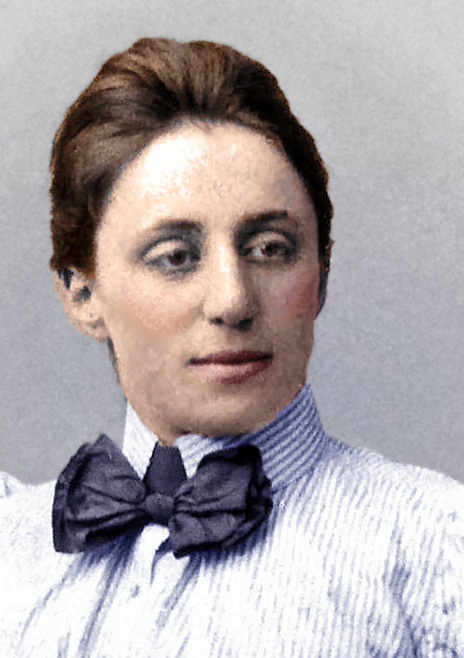
\includegraphics[scale=1]{img/Noether.jpg}
 \captionsetup{labelformat=empty}
 \caption{埃米$\cdot$诺特 1882-1935}
 \label{fig:Noether}
%\end{figure}
\end{wrapfigure}

\index{诺特(Emmy Noether)}
现代抽象数学中环和域的概念是由德国女数学家埃米$\cdot$诺特所发展的。1882年3月23日,诺特生于德国大学城埃尔朗根的一个犹太人家庭。她的父亲是埃尔朗根大学的数学家。诺特本来打算将来教授法文和英文,但在父亲的影响下,她逐渐对数学产生了兴趣。1900年冬天,18岁的诺特考进了埃尔朗根大学。当时,大学里不允许女生注册,女生顶多只有自费旁听的资格。大学的986名学生中只有两名女生,诺特大大方方地坐在教室前排,认真听课,刻苦学习,后来,她勤奋好学的精神感动了主讲教授,破例允许她与男生一样参加考试。1903年7月,诺特顺利通过了毕业考试,男生们都取得了文凭,而她却成了没有文凭的大学毕业生。诺特生活在公开歧视妇女发挥数学才能的制度下。毕业以后她在埃尔朗根数学研究院工作,长达7年却没有任何工资。1907年12月,她以优异的成绩通过了博士考试,成为第一位女数学博士。此后,她在著名的数学家高丹、费叶尔的指引下,在数学的不变式领域进行了深入的研究。1915年,应著名数学家希尔伯特和克莱因的邀请,诺特来到数学圣地哥廷根大学。不久,她就以希尔伯特教授的名义,在哥廷根大学讲授数学课程。希尔伯特十分欣赏诺特的才能,想帮她在哥廷根大学找一份正式的工作。当时的哥廷根大学没有专门的数学系,数学、语言学、历史学都划在哲学系里,聘请必须经过哲学教授会议批准。希尔伯特的努力遭到教授会议中语言学家和历史学家的极力反对,他们出于对妇女的传统偏见,连聘为“私人讲师”这样的请求也断然拒绝。希尔伯特屡次据理力争都没有结果,他在一次教授会上愤愤地说:“我简直无法想象候选人的性别竟成了反对她升任讲师的理由。先生们,别忘了这里是大学而不是洗澡堂!”

在希尔伯特等人的影响下,不到两年时间,诺特就发表了两篇重要论文。诺特为爱因斯坦的广义相对论给出了一种纯数学的严格方法。并提出了现代物理学中称为“诺特定理”的观点。就这样,诺特以她出色的科学成就,迫使那些歧视妇女的人也不得不于 1919年准许她升任讲师。此后,诺特走上了完全独立的数学道路。1921年,她从不同领域的相似现象出发,把不同的对象加以抽象化、公理化,然后用统一的方法加以处理,完成了《环中的理想论》这篇重要论文。这是一项非常了不起的数学创造,它标志着抽象代数学真正成为一门数学分支,或者说标志着这门数学分支现代化的开端。诺特也因此获得了极大的声誉,被誉为是“现代数学代数化的伟大先行者”,“抽象代数之母”。1931年,她的学生荷兰数学家的范德瓦尔登系统总结了整个诺特学派的成就,出版了《近世代数》一书,影响了许多当时的青年数学家。1932年,诺特的科学声誉达到了顶点。在这一年于苏黎世举行的第9届国际数学家大会上,诺特作了长达1小时的大会发言,受到广泛的赞扬。

然而,巨大的声誉并未改善诺特的艰难处境。在不合理的制度下,灾难和歧视像影子一样缠住了她。1922年,由于大数学家希尔伯特等人的推荐,诺特终于在清一色的男子世界——哥廷根大学取得教授称号。不过,那只是一种编外教授,没有正式工资,于是,这位历史上最伟大的女数学家,只能从学生的学费中支取一点点薪金,来维持极其简朴的生活。希特勒上台后,德国法西斯对犹太人的迫害愈演愈烈。1929年,诺特被撵出居住的公寓。1933年4月,法西斯当局剥夺了诺特教书的权利,将一批犹太人教授逐出校园,诺特只好辗转逃往美国。尽管她是世界知名的数学家,但由于是女性,诺特没有获得大型研究院校的聘约。最后,她在一家名为布林莫尔(Bryn Mawr)的女校以访问学者的身份任教。1935年,诺特做了卵巢囊肿摘除手术,4月14日不幸去世,终年53岁。

诺特善于通过透彻的洞察建立优雅的抽象概念,再将之漂亮地形式化。被帕维尔·亚历山德罗夫、爱因斯坦、迪厄多内、外尔和维纳形容为数学史上最重要的女性。她彻底改变了环、域和代数的理论。在物理学方面,诺特定理解释了对称性和守恒定律之间的根本联系,她还被称为“现代数学之母”,她允许学者们无条件地使用她的工作成果,也因此被人们尊称为“当代数学文章的合著者”\cite{Wiki-Noether}。

\subsection{环的定义}
\index{环}
群是定义了一种运算的系统(集合与乘法运算),而环(ring)是定义了两种运算的系统。给定元素$a, b, ...$的集合$R$,并在之上定义加法$a+b$和乘法$ab$,它们的结果也都属于这个集合。其中加法和乘法满足下面的规律:

\begin{enumerate}
\item 加法的规律:
  \begin{enumerate}
  \item 结合律: $a + (b + c) = (a + b) + c$
  \item 交换律: $a + b = b + a$
  \item 存在唯一的单位元,任何元素都有唯一逆元。
  \end{enumerate}
\item 乘法的规律:
  \begin{enumerate}
  \item 结合律: $a(bc) = (ab)c$
  \end{enumerate}
\item 分配律:
  \begin{enumerate}
  \item $a(b + c) = ab + ac$
  \item $(b + c)a = ba + ca$
  \end{enumerate}
\end{enumerate}

可以看出加法系统构成一个群,并且由于满足交换律,所以是一个阿贝尔加群。而乘法只是封闭的满足结合律的半群。

\index{交换环}
显然,全体整数对于普通加法和乘法构成一个环。另外多项式和矩阵对于加法和乘法也构成一个环。在环的定义中,我们只要求加法满足交换律,构成阿贝尔群。而对乘法没有要求。如果乘法也满足交换律,我们称这样的环为\textbf{交换环}。在一个交换环里,对于正整数$n$和任何两个元都有:

\[
a^nb^n = (ab)^n
\]

在环的定义中,我们也没有要求环中的乘法一定要有单位元。如果$R$中存在一个元素$e$的,使得对任何元素都有:

\[
ea = ae = a
\]

则称$e$为环的单位元。一般来说,一个环未必有单位元\footnote{现代学者更多使用包含乘法单位元的环定义,因为这样可以涵盖更为丰富有趣的代数结构。而用符号$rng$来表示不含乘法单位元的环。}。习惯上我们常用1来代表乘法单位元(unity),用0代表加法单位元。当然它们只是符号,并不是数字0、1。有了单位元,自然也可以规定逆元。如果$ab = ba = 1$,我们称$b$是$a$的逆元。从群的性质我们可以推知,如果一个环有单位元,这个单位元必然是唯一的。如果一个元素有逆元,这个逆元也必然是唯一的。但是并非任何元素都逆元,例如整数环有单位元,但除了$\pm 1$外,其它整数都没有逆元。在环中,我们称有逆元的元素为可逆元(unit)。

由于环上有分配律,所以我们有:

\[
(a - a)a = a(a - a) = aa - aa = 0
\]

因此

\[
0 a = a 0 = 0
\]

也就是说,环中两个元$a$、$b$之中,如果有一个是0,则$ab = 0$。但是这一结论的逆命题却不成立。也就是说,由$ab = 0$,并不能推知$a$或$b$中存在一个0。我们来看一个反例。考虑模$n$的剩余类,其中加法是模$n$的加法:$[a] + [b] = [a + b]$,即相加后对$n$取模,其构成一个交换加群。模$n$的乘法定义为:$[a][b] = [ab]$,即相乘后对$n$取模。容易验证这构成一个环,称为模$n$的剩余类环。

如果$n$不是素数,例如10,我们发现两个非0元素$[5][2] = [5 \times 2] = [0]$。事实上,把$n$分解成两个因子,其模乘的结果必然是零。

\index{零因子}
在一个环里,如果$a \neq 0, b \neq 0$,但却有$ab = 0$,我们说$a$是环的一个\textbf{左零因子},$b$是环的一个\textbf{右零因子}。如果环是交换环,那么一个左零因子同时也是右零因子。当然,一个环可能没有零因子,例如整数环。只有在没有零因子的环里,我们才能从$ab = 0$推知$a$或$b$等于0。并且我们有如下定理:

\begin{theorem}
一个没有零因子的环里,以下两个消去律都成立:
\begin{itemize}
\item 若$a \neq 0$,$ab = ac$,则$b = c$
\item 若$a \neq 0$,$ba = ca$,则$b = c$
\end{itemize}
\end{theorem}

反之,如果一个环里任一个消去律成立,则另一个也必然成立,并且环中没有零因子。

\index{整环}
这样,我们认识了一个环的三种附加条件:一是乘法满足交换律;二是单位元存在;三是不存在零因子。同时满足这三个附加条件的环有一个特殊名称,叫做\textbf{整环}(integral domain)。整数环显然是一个整环。

\index{半环}
有些情况下,环的条件太强了。我们并不需要加法一定存在逆元(即加法取反,additive inverse)。如果放宽条件,我们就得到\textbf{半环}这种代数结构。

\begin{definition}
一个集合$R$,以及其上定义的某种加法和乘法称作半环,如果它满足以下条件。
\begin{enumerate}
\item $R$上的加法构成一个交换幺半群,并且存在一个称为0的单位元;
\item $R$上的乘法构成了一个幺半群,并且存在一个称为1的单位元;
\item 满足分配律,任意$a, b, c$都有:
\[
\begin{array}{l}
a(b + c) = ab + ac \\
(b + c)a = ba + ca
\end{array}
\]
\item 0元乘以任何元都得0。即$a0 = 0a = 0$
\end{enumerate}
\end{definition}
自然数$N$就是半环的典型例子。布尔运算是一个只有两个元素的半环。

\begin{Exercise}
\Question{证明本节的定理,一个没有零因子的环里,两个消去律成立。}
\Question{证明所有形如$a + b \sqrt{2}$,其中$a, b$是整数的实数对于普通加法和乘法构成一个整环。}
\end{Exercise}

\subsection{除环和域}

我们知道一个环里不一定所有的元素都有逆元。如果某个环中所有的非零元素都有逆元,就构成一种特殊的环。例如全体有理数对于普通加法和乘法来说显然是一个环,这个环中任意不等于零的元$a$都有逆元$\dfrac{1}{a}$。

\index{除环}
\begin{definition}
一个环$R$如果满足以下条件,则叫做\textbf{除环}:
\begin{enumerate}
\item $R$至少包含一个不等于零的元;
\item $R$有一个单位元1;
\item $R$的每个不等于零的元都有一个逆元。
\end{enumerate}
\end{definition}

\index{域}
\begin{definition}
一个交换除环叫做一个\textbf{域}。
\end{definition}

按照这一定义,全体有理数构成一个域。同样,全体实数或者全体复数的集合对于普通加法和乘法也各自构成一个域\footnote{我们在第6章会看到,有理数域是可数的,而实数、复数域是不可数的}。除环和域有一些有趣的性质。一个除环没有零因子。这是因为,如果$a \neq 0$,并且$ab = 0$。我们在两边左乘$a$的逆元:

\[
a^{-1}ab = b = 0
\]

这样必然有$b$等于零,所以除环不含有零因子。第二个性质是,一个除环中的所有非零元,对于乘法构成一个群$R*$,我们称$R*$叫做除环$R$的乘群。这样一个除环是由两个群:加群与乘群组合而成的;分配率好像是一座桥梁,使得两个群发生联系。到目前为止,我们介绍过的环、半环、整环、除环和域的关系总结如图\ref{fig:ring}。

\begin{figure}[htbp]
\centering
\begin{tikzpicture}[scale=0.8]
\draw (0, 1) node (semiring) {半环}
      (0, 0) node (ring) {环}
      (-4, -1) node (commu-ring) {交换环}
      (0, -1) node (unit) {有单位元}
      (3, -1) node (zero-factor) {无零因子}
      (-3, -3) node (integral-domain) {整环}
      (3, -3) node (division-ring) {除环}
      (0, -4) node (field) {域};
\draw (0, 2) circle[x radius = 1.5cm, y radius = 0.5cm] node (add-monoid) {加法幺半群}
      (4, 2) circle[x radius = 1.5cm, y radius = 0.5cm] node (mul-monoid) {乘法幺半群}
      (-4, 2) circle[x radius = 1.5cm, y radius = 0.5cm] node (distribution-law) {分配律}
      (4, 0.5) circle[x radius = 1.5cm, y radius = 0.5cm] node (negate) {加法可求反}
      (-5, 0) circle[x radius = 1.5cm, y radius = 0.5cm] node (mul-commu) {乘法可交换}
      (0, -3) circle[x radius = 1.5cm, y radius = 0.5cm] node (mul-invert) {乘法可求逆};
\draw (distribution-law) to (semiring)
      (add-monoid) to (semiring)
      (mul-monoid) to (semiring)
      (semiring) to (ring)
      (negate) to (ring)
      (mul-commu) to (commu-ring)
      (ring) to (commu-ring)
      (ring) to (unit)
      (ring) to (zero-factor)
      (commu-ring) to (integral-domain)
      (unit) to (integral-domain)
      (zero-factor) to (integral-domain)
      (unit) to (division-ring)
      (zero-factor) to (division-ring)
      (integral-domain) to (field)
      (division-ring) to (field)
      (mul-invert) to (division-ring);
\end{tikzpicture}
\caption{半环、环、整环和域}
\label{fig:ring}
\end{figure}

还有一些重要的概念,如子环、理想、主理想环与欧几里得环限于篇幅我们不在这里介绍了。

\section{伽罗瓦理论}
我们分别介绍了域和群,而伽罗瓦理论像是一座桥梁把它们连接到了一起。域里面有加减乘除四种运算和无穷多个元素,是很复杂的对象。而伽罗瓦理论可以把域中的一些问题化简到只有一种运算的有限群里去。整个伽罗瓦理论的核心思想就是这一点。

伽罗瓦理论无疑是相当艰深难懂的。今天我们读到的伽罗瓦理论不再模糊费解,而是经过不下二十位大师的发展和处理的。其中最主要的贡献当属若当、戴德金和阿廷。若当和戴德金分别在法国和德国最早系统地整理伽罗瓦理论。今天使用的伽罗瓦群的定义是由戴德金给出的。阿廷使得伽罗瓦理论取得了现代的形式\cite{ZhangPu2013}。为了在这么短的一个章节介绍伽罗瓦理论,我采用了对初学者比较容易理解的一种解释\cite{Stillwell1994}。对于一般的读者,可能仍然无法一遍就弄懂它。开卷有益,生活不是线性发展的。我建议大家不断回过头去重温此前介绍的一些概念,并阅读那些名著。每次也许有不同的体会,让我们一起享受那种一览众山小的感觉。

\subsection{扩域}
\index{扩域}
根据域的定义,我们知道全体有理数构成一个域,记作$Q$。我们现在考虑所有形如$a + b\sqrt{2}$的数组成的集合,其中$a, b$都是有理数\cite{Goodman2011}。显然有理数是这一集合的子集(只要让$b=0$即可)。容易验证,任何两个这样的数做加、减、乘法都仍然可以写成$a + b \sqrt{2}$的形式。除法稍微难些。观察$x = \dfrac{1}{a + b\sqrt{2}}$,我们可以将分子分母同时乘以$a - b \sqrt{2}$,这样就有:

\[
\begin{array}{rl}
x & = \dfrac{a - b \sqrt{2}}{(a + b \sqrt{2})(a - b \sqrt{2})} \\[2ex]
  & = \dfrac{a - b \sqrt{2}}{a^2 - 2b^2}
\end{array}
\]

令$p = a^2 - 2b^2$,这样$x$就可以表示成$(a/p) -(b/p)\sqrt{2}$。这样除法也就验证了。的的确确这一集合构成一个域。我们将其记为$Q[\sqrt{2}]$。同理$Q[\sqrt{3}]$也是一个域。这就引出了扩域的概念。

\begin{definition}
如果域$E$包含域$F$,我们称$E$是$F$的\textbf{扩域},记作$F \subseteq E$或者$E/F$。
\end{definition}

例如实数域就是有理数域的扩域,$Q[\sqrt{2}]$是有理数域$Q$的扩域。一般来说,如果$F$是一个域,$\alpha \in F$,但是$\sqrt{\alpha} \not\in F$,则$F_1 = F[\sqrt{\alpha}]$仍是一个域。这样,我们就可以重复使用这个方法不断扩张。若$\beta \in F_1$, 但$\sqrt{\beta} \not\in F_1$,则:

\[
\begin{array}{rl}
F_2 & = F_1[\sqrt{\beta}] \\
    & = F[\sqrt{\alpha}][\sqrt{\beta}] \\
    & = F[\sqrt{\alpha}, \sqrt{\beta}]
\end{array}
\]

即所有形如$a + b \sqrt{\beta}$的数,其中$a, b \in F_1$的数构成了更高层次的扩域。这样我们就可以从有理数域开始,得到一个扩域系列:$Q \subset F_1 \subset F_2 ... \subset F_n$。

扩域有何意义呢?举个例子,方程$x^2 - 2 = 0$在有理数域上无解,但是它在有理数域的扩域$Q[\sqrt{2}]$上有一对解($x = \pm \sqrt{2}$)。我们进一步再看一个例子,方程$x^4 - 5x^2 + 6 = 0$在有理数域上无解,在扩域$Q[\sqrt{2}]$上有两个解$\pm \sqrt{2}$,在扩域$Q[\sqrt{2}, \sqrt{3}]$上有全部四个解$\pm \sqrt{2}, \pm \sqrt{3}$。于是就自然引出了根域的重要概念:

\index{分裂域} \index{根域}
\begin{definition}
包含方程$p(x) = 0$全部根的最小扩域叫做$p(x)$的\textbf{分裂域}。也称为根域。
\end{definition}

这样方程$x^2 -2 = 0$的分裂域就是$Q[\sqrt{2}]$。为什么叫做“分裂”呢?多项式$x^2-2$在有理数域$Q$上是不可约的,但是在扩域$Q[\sqrt{2}]$上可以“分裂”成:
\[
(x + \sqrt{2}) (x - \sqrt{2})
\]
对于某一多项式方程,如果我们能够从基本域有理数域开始,通过一系列上述的扩域,最终到达分裂域,那么自然这个方程是可以用根式解的。

我们给出了平方根的例子,显然还有更加复杂的情况。例如此前介绍的分圆方程$x^p-1=0$含有$p$个根$1, \zeta, \zeta^2, ..., \zeta^{p-1}$,它们分布在复平面的单位圆上。为了涵盖这些情况,我们需要更加严格地描述扩域。

%% \begin{figure}[htbp]
%% \centering
%% \begin{tikzpicture}[scale=3]
%%  \draw[step=.5cm, gray, very thin] (-1.2,-1.2) grid (1.2,1.2);
%%  \draw[->] (-1.25,0) -- (1.25,0) coordinate (x axis);
%%  \draw[->] (0,-1.25) -- (0,1.25) coordinate (y axis);
%%  \draw (0,0) circle (1cm);
%%  \draw[->, very thick] (0, 0) edge node[below=2pt,fill=white] {$\zeta^0 = \zeta^3 = 1$} (1, 0)
%%      (0, 0) edge node[above] {$\zeta = \dfrac{-1 + i\sqrt{3}}{2}$} (120:1cm)
%%      (0, 0) edge node[below] {$\zeta^2 = \dfrac{-1 - i\sqrt{3}}{2}$} (-120:1cm);
%% \end{tikzpicture}
%% \caption{单位根,$x^3 - 1 = 0$}
%% \label{fig:root-of-unity}
%% \end{figure}

\index{正规扩域}
如果$\alpha$的整数次方等于域$F$中的某个元素$b$,也就是说$\alpha^m = b \in F$,这样$\alpha$就可以写成$b$的根式形式$\alpha = \sqrt[m]{b}$。为了简化问题,假设每次根式扩域$F[\alpha_i]$中加入的$\alpha_i$都是素数次方根。例如对$\sqrt[6]{\alpha}$,我们把它拆成$\sqrt{\alpha} = \beta$和$\sqrt[3]{\beta}$,然后分两次进行根式扩域。还有一个问题需要解决,考虑方程$x^3 - 2 = 0$,仅仅将$\sqrt[3]{2}$加入域中是不够的。方程的另外两个根$\omega\sqrt[3]{2}, \omega^2\sqrt[3]{2}$不在扩域$Q[\sqrt[3]{2}]$中。为此我们需要同时加入$\sqrt[3]{2}$和$\omega = \dfrac{-1 + i\sqrt{3}}{2}$,形成扩域$Q[\sqrt[3]{2}, \omega]$。这样的扩域包含多项式的\textbf{所有}根,我们将这样的扩域称为正规扩域。

\index{根式扩域}
我们可以逐一用这样的一组根式进行扩域,从而得到$F[\alpha_1][\alpha_2]...[\alpha_k]$。如果每次扩张所用的$\alpha_i$都是根式,我们称扩域$F[\alpha_1, \alpha_2, ..., \alpha_k]$为$F$的根式扩域(radical extension)。设方程的根是$x_1, x_2, ..., x_n$(注意,这里我们没有说$x_i$一定是根式),如果其分裂域$E = Q[x_1, x_2, ..., x_n]$是根式扩域,我们说方程是根式可解的。

\begin{Exercise}
\Question{证明$Q[a, b] = Q[a][b]$,其中$Q[a, b]$是所有由$a, b$组成的表达式如$2ab, a + a^2b$等。}
\end{Exercise}

\subsection{从牛顿、拉格朗日到伽罗瓦}

人类理性和认知的进步是共同努力的结果。伽罗瓦理论这颗智慧的明珠不是凭空出现的。沿着它背后的历史脉络,我们能看到一系列的脚步:从韦达、牛顿、范德蒙德、拉格朗日、到高斯,最终在伽罗瓦手中结出了灿烂的成果。回溯历史,能让我们更好地理解伽罗瓦是如何形成他的思路的。

\subsubsection{对称多项式与牛顿定理}
\index{对称多项式}
人们熟悉牛顿那些最伟大的发现,包括微积分、二项式定理、经典力学。他其实在很多领域都取得了惊人的成果。韦达之后,牛顿深入思考了更多的对称多项式,他的结果发表在1707的著作《普遍算数》中。高斯称之为“牛顿定理”。牛顿的性格很难被今天的人们所理解,他迟迟不肯发表自己的发现。如果不是哈雷的鼓动和催促,他根本不愿意出版《自然哲学的数学原理》。牛顿定理也是如此,人们在他23岁(1665或1666)时的笔记中发现了这些结果:

令三次方程$x^3 + bx^2 + cx + d = 0$的3个根为$r, s, t$,等式

\[
x^3 + bx^2 + cx + d = (x - r)(x - s)(x -t)
\]

成立,并且:

\bea*{rcl}
r + s + t & = & -b \\
r^2 + s^2 + t^2 & = & b^2 - 2c \\
r^3 + s^3 + t^3 & = & -b^3 + 3bc - 3d \\
rs + st + rt & = & c \\
r^2s + s^2t + t^2r + r^2t + t^2s + s^2r = -bc + 3d \\
... & & ... \\
r^3s^3t^3 = -d^3
\eea*

牛顿列出了19个对称多项式的结果,他还把方程的次数增加到8次$x^8 + px^7 + qx^6 + rx^5 + sx^4 + tx^3 + vx^2 + yx + z = 0$进行类似的计算。牛顿发现这些对称多项式中,有一些是基本的。推广到$n$次方程的$n$个根:

\[
x^n + b_1 x^{n-1} + b_2 x^{n-2} + ... + b_n = (x - r_1)(x - r_2)...(x - r_n)
\]

这些基本对称多项式为:
\index{基本对称多项式}

\bea{rcccl}
\sigma_1 & = & r_1 + r_2 + ... + r_n & = & -b_1 \\
\sigma_2 & = & r_1r_2 + r_2r_3 + ... + r_{n-1}r_n & = & b_2 \\
\sigma_3 & = & r_1r_2r_3 + r_1r_2r_4 + ... + r_{n-2}r_{n-1}r_n & = & -b_3 \\
& & ... & & \\
\sigma_n & = & r_1r_2...r_n & = & (-1)^nb_n \\
\eea

为什么说它们是基本对称多项式呢?因为牛顿发现任何对称多项式都可以变换基本对称多项式的组合。例如:$(a - b)$并不是对称的(交换$a,b$值的正负会改变),平方后$(a - b)^2$是对称多项式,它可以变换为:

\bre
(a - b)^2 & = & (a + b)^2 - 4ab & \text{变成两个对称多项式相减} \\
          & = & \sigma_1^2 - 4\sigma_2 & \text{二次方程基本对称多项式} \\
\ere

\begin{theorem}
\textbf{牛顿定理}:任何关于$r_1, r_2, ..., r_n$的对称多项式都可用基本对称多项式$\sigma_1, \sigma_2, ..., \sigma_n$来表示。
\end{theorem}
\index{牛顿定理}

\subsubsection{拉格朗日预解式}
\index{拉格朗日预解式}
我们略去了牛顿定理的证明。沿着牛顿对称多项式的思路继续向前迈进的是法国数学家范德蒙德和拉格朗日。他们两个各自进行独立研究。拉格朗日并不了解范德蒙德的工作,但是他解决三次方程的方法本质上和范德蒙德是一致的。拉格朗日的论文长达220页,我们只能简单总结一下他的结果(正是伽罗瓦15岁时研读并掌握的那篇《关于方程代数解的思考》\footnote{1770年的论文Réflexions sur la résolution algébrique des équations})。首先一般三次方程$ay^3 + by^2 + cy + d = 0$,可以进行变量替换,令$y = x - b / 3a$,将其转换为$x^3 + px + q = 0$的形式。如果它的三个根为$r_1, r_2, r_3$,拉格朗日把3次本原单位根$\omega = \dfrac{-1 + i \sqrt{3}}{2}$也考虑进来。根据分圆方程的结果,我们有$\omega^3 = 1, 1 + \omega + \omega^2 = 0$。拉格朗日引进了一个关键概念——预解式(resolvent),令:

\be
t = r_1 + \omega r_2 + \omega^2 r_3
\ee

拉格朗日对三个根进行置换(重新排列),他发现了一个有趣的现象,尽管总共有6种置换,但是预解式$r$的立方却只有两个值。1770年还没有群的概念,我们今天知道,拉格朗日发现的,本质上是在群$S_3$的6个置换下,预解式$r^3$只有2个值:

\[
\begin{cases}
t_1^3 = (r_1 + \omega r_2 + \omega^2 r_3)^3 = L^3 & (1) \\
t_2^3 = (\omega r_1 + \omega^2 r_2 + r_3)^3 = (\omega L)^3 = L^3 & (132) \\
t_3^3 = (\omega^2 r_1 + r_2 + \omega r_3)^3 = (\omega^2 L)^3 = L^3 & (123) \\
\end{cases}
\]

其中左边是预解式的值,右边是$S_3$中的置换。因为$\omega^3 = 1$,以上面第二行为例:$r_3 \omega^3 = r_3$。可以看出这一组是同时置换3个根,对应着不变子群$C_3$中的置换$\{(1), (132), (123)\}$,

\[
\begin{cases}
t_4^3 = (r_1 + \omega^2 r_2 + \omega r_3)^3 = R^3 & (23) \\
t_5^3 = (\omega r_1 + r_2 + \omega^2 r_3)^3 = (\omega R)^3 = R^3 & (12) \\
t_6^3 = (\omega^2 r_1 + \omega r_2 + r_3)^3 = (\omega^2 R)^3 = R^3 & (13) \\
\end{cases}
\]

这一组的特点是固定一个根而交换另外两个根,对应着陪集中的置换$\{(23), (12), (13)\}$。拉格朗日接着引入了预解式方程:

\be
(X - t_1)(X - t_2)(X - t_3)(X - t_4)(X - t_5)(X - t_6) = 0
\ee

这个看似复杂的6次方程实际上可以化为2次方程。前三个因式一组,后三个因式一组。其中$(X - t_1)(X - t_2)(X - t_3) = (X - L)(X - \omega L) (X - \omega^2 L) = X^3 - L^3$,同样后三个因式化简为$X^3 - R^3$,这样预解式方程就变成了$(X^3 - L)(X^3 - R) = 0$。进一步展开得:

\be
X^6 - (L^3 + R^3)X^3 + L^3R^3 = 0
\ee

将$X^3$替换为$Y$,就变成了二次方程$Y^2 -(L^3 + R^3)Y + L^3R^3 = 0$。预解式的立方和与积能用原方程的系数表示:

\be
\begin{cases}
L^3 + R^3 = -27q \\
L^3R^3 = -27p^3 \\
\end{cases}
\label{eq:LR-pq}
\ee

代入$p, q$,解关于$Y$的二次方程就可以求出$L, R$了。回顾方程$x^3 + px + q = 0$,由于2次项为0,所以根据韦达定理。我们有$r_1 + r_2 + r_3 = 0$。这样我们可以联立出3个方程:

\be
\begin{cases}
r_1 + \omega r_2 + \omega r_3 = L \\
r_1 + \omega^2 r_2 + \omega r_3 = R \\
r_1 + r_2 + r_3 = 0 \\
\end{cases}
\ee

解方程组就得到了用拉格朗日预解式表达的3个根:

\be
\begin{cases}
r_1 = \dfrac{\omega^2 L + \omega R}{3} \\
r_2 = \dfrac{\omega L + \omega^2 R}{3} \\
r_3 = \dfrac{L + R}{3} \\
\end{cases}
\ee

再代入求出的$L, R$就解出了3次方程的根。拉格朗日的方法具有重要的启示。以4次方程为例,结合4次单位根$\pm 1, \pm i$,定义预解式:

\be
t = r_1 + i r_2 - r_3 - i r_4
\ee

在4阶对称群$S_4$的$4! = 24$个置换下,下面预解式方程是不变的:

\be
\Phi(X) = (X - t_1)(X - t_2)...(X - t_{24})
\ee

根据牛顿定理,它的所有系数已知。拉格朗日成功地把这个24次方程,简化为3次方程,然后加以解决。然而拉格朗日被5次方程卡住了。此时预解式$\Phi(X) = (X - r_1)(X - r_2) ... (X - r_{120})$达到了$5! = 120$次。拉格朗日把它转换成了低次的5次方程,但这相当于转了一圈又回到了5次方程的问题。接下来的关键一步需要等到伽罗瓦迈出。

\subsubsection{伽罗瓦的遗稿}
\index{不可约多项式} \index{最小多项式}

我们把时光倒转到1832年5月29日深夜,尝试理解这篇沉重的论文。我们略去了证明,通过一些验证性的例子展示伽罗瓦的主要思路。伽罗瓦首先定义了什么是不可约多项式:多项式$f(x)$的系数域\footnote{当时还没有域的概念,后来德国数学家戴德金定义了域。}为$F$,如果$f(x)$可以在域$F$内因式分解,称其为可约的,否则叫做不可约多项式。例如$x^2 + 1$在有理数域$Q$内是不可约的,但是在复数域$C$内可以因式分解为$(x + i)(x - i)$。再例如$x^2 - 2$在有理数域$Q$内是不可约的,但是在扩域$Q[\sqrt{2}]$内可分解为$(x + \sqrt{2})(x - \sqrt{2})$。域$F$上以某个值为根,最高次系数为1(简称“首1”),并且次数最低的不可约多项式叫做最小多项式。例如$x^2 - 2$就是有理数域上,以$\sqrt{2}$为根的最小多项式。伽罗瓦接着定义什么是已知的数,从有理数域开始,通过向其中添加指定的数,并通过有理式(也就是四则运算)得到的数叫做已知的。我们今天知道,这相当于扩域的概念。

伽罗瓦接下来引入了置换群的概念。这是对若干元素重新排列的群。他第一个给出了法文groupe这个词,并且指出两个置换组合起来的结果也是一个置换。在今天看来,伽罗瓦使用的是置换群$S_n$的及其子群。有了置换群,伽罗瓦就可以对方程根组成的有理式进行置换。例如有理式$x_1 x_2 + x_3$,使用$\sigma = (123)$进行置换后得到:

\[
\sigma(x_1 x_2 + x_3) = x_2 x_3 + x_1
\]

接下来伽罗瓦给出了不可约多项式的性质:

\begin{lemma}不可约多项式的性质:设$f(x)$为域$F$上的多项式,$p(x)$为域$F$上的不可约多项式。如果$f(x)$和$p(x)$有共同的根,则$f(x)$可以被$p(x)$整除。
\end{lemma}

我们可以类比这个性质和整数的整除性质:多项式相当于整数,不可约多项式相当于素数。有共同的根相当于含有相同的素因子。例如多项式$f(x) = x^3 - 1$,在有理数域上$p(x) = x^2 + x + 1$是不可约多项式。它们两个有共同的根$\omega = \dfrac{-1 + i\sqrt{3}}{2}$:

\[
\omega^3 - 1 = \omega^2 + \omega + 1 = 0
\]

$f(x)$的确可以被$p(x)$整除:$x^3 - 1 = (x - 1)(x^2 + x + 1)$。

伽罗瓦接下来的思路,看起来像是拉格朗日预解式的延伸,他定义了“伽罗瓦预解式”。

\begin{lemma}伽罗瓦预解式$t$:设$f(x)$是域$F$上的多项式,它的根为$x_1, x_2, ..., x_n$。存在根的某个有理式$t = \varphi(x_1, x_2, ..., x_n)$,在根的不同排列下取不同的值。
\end{lemma}

也就是说,置换$n$个根产生的不同排列,导致各种不同的$t$值。例如,有理数域上的多项式$f(x) = x^2 + 1$有两个根$x_1 = i, x_2 = -i$。我们可以找到一个有理式:

\[
t = x_1 - x_2
\]

在$S_2$的两个置换(1)和(12)下$t$取不同的值:

\[
\begin{cases}
t_1 = x_1 - x_2 = 2i & \text{对应置换} (1) \\
t_2 = x_2 - x_1 = -2i & \text{对应置换} (12) \\
\end{cases}
\]

这两个值不相等。伽罗瓦只是说存在$t$。他说可以通过根的整系数线性组合构造$t = k_1x_1 + k_2x_2 + ... + k_nx_n$,但是没有给出证明。伽罗瓦还排除了重根的情况,因为重根不管怎么排列都是一样的。回忆拉格朗日的方法是用预解式不同值表达方程的根,伽罗瓦也延续这个思路。

\begin{lemma}用伽罗瓦预解式$t$表示根:域$F$上存在有理式$\varphi_1(x), \varphi_2(x), ..., \varphi_n(x)$, 使得多项式$f(x)$的根$x_1, x_2, ..., x_n$可以用伽罗瓦预解式$t$表示为:
\[
x_1 = \varphi_1(t), x_2 = \varphi_2(t), ..., x_n = \varphi_n(t)
\]
\end{lemma}

还用上面的例子,$f(x) = x^2 + 1$,两个根是$x_1 = i, x_2 = -i$,预解式$t = x_1 - x_2 = 2i$,我们可以找到$\varphi_1(x) = \dfrac{x}{2}, \varphi_2(x) = -\dfrac{x}{2}$,用$t$表示两个根如下:

\[
x_1 = \dfrac{t}{2}, x_2 = -\dfrac{t}{2}
\]

这样伽罗瓦就把方程个根域$F[x_1, x_2, ..., x_n]$和扩域$F[t]$联系了起来。置换$n$个根的时候,伽罗瓦预解式$t$会产生不同的值。延续拉格朗日的思路,$t$是另外一个预解方程$f_t(X) = 0$的某个根(一个方程可能有多个根)。

\begin{lemma}
在域$F$内构造一个以$t$为根的最小多项式$f_t(X)$,设$f_t(X)$的根为$t_1, t_2, ..., t_m$,此时
\[
\varphi_1(t_k), \varphi_2(t_k), ..., \varphi_n(t_k)
\]
是原方程$f(x) = 0$根的某种排列($k = 1, 2, ..., m$)。
\end{lemma}

注意这里的区别$f(x) = 0$是原方程,而$f_t(X) = 0$是构造出的方程。其中$f_t(X)$是以$t$为其中一个根最小多项式。原方程有$n$个根$x_1, ..., x_n$,预解式方程有$m$个根$t_1, t_2, ..., t_m$

\[
(X - t_1)(X - t_2)...(X - t_m) = 0
\]

它们彼此的关系是: $t = \varphi(x_1, ..., x_n)$,而$x_i = \varphi_i(t)$。作为例子,考虑方程$x^3 - x^2 - 2x + 2 = 0$,它有3个根$1, \pm \sqrt{2}$。第一步构造伽罗瓦预解式:$t = \varphi(x_1, x_2, x_3) = x_1 + 2x_2 + 4x_3$。它在$S_3$下的取6个不同的值:

\btab{c|c|l}
置换 & $\varphi(x_1, x_2, x_3)$ & $t$ \\
\hline
(1, 2, 3) & $x_1 + 2x_2 + 4x_3$ & $1 - 2\sqrt{2}$ \\
(1, 3, 2) & $x_1 + 2x_4 + 4x_2$ & $1 + 2\sqrt{2}$ \\
(2, 1, 3) & $x_2 + 2x_1 + 4x_3$ & $2 - 3\sqrt{2}$ \\
(2, 3, 1) & $x_2 + 2x_3 + 4x_1$ & $4 - \sqrt{2}$ \\
(3, 1, 2) & $x_3 + 2x_1 + 4x_2$ & $2 + 3\sqrt{2}$ \\
(3, 2, 1) & $x_3 + 2x_2 + 4x_1$ & $4 + \sqrt{2}$ \\
\etab

第二步,取$t = 1 - 2\sqrt{2}$和前三行,可以联立出方程组:

\[
\begin{cases}
x_1 + 2x_2 + 4x_3 & = 2t \\
x_1 +  x_3 + 4x_2 & = 2 - t \\
x_2 + 2x_1 + 4x_3 & = \dfrac{3t + 1}{2}
\end{cases}
\]

解方程组得到用$t$表示的三个根:

\[
\begin{cases}
x_1 = \varphi_1(t) = 1 \\
x_2 = \varphi_2(t) = \dfrac{1-t}{2} \\
x_3 = \varphi_3(t) = \dfrac{t-1}{2} \\
\end{cases}
\]

第三步,构造以$t = 1 - 2\sqrt{2}$为根的最小多项式:$f_t(X) = X^2 - 2X - 7$。它有两个根:$t_{1,2} = 1 \pm 2\sqrt{2}$。代入$\varphi_1(t), \varphi_2(t), \varphi_3(t)$得到根的两个置换:

\btab{c|c|c}
$t_i$ & $\varphi_1(t_i), \varphi_2(t_i), \varphi_3(t_i)$ & $S_3$中的置换 \\
\hline
$t_1$ & $1, \sqrt{2}, -\sqrt{2}$ & (1) \\
$t_2$ & $1, -\sqrt{2}, \sqrt{2}$ & (23) \\
\etab

我们可以看到拉格朗日思想的影响。但伽罗瓦预解式不是特定构造出的,而是某种“存在性”定义。他的预解式方程也是用最小多项式给出的“存在性”定义。这里有一个和拉格朗日方法的不同点,$m$并不一定等于$n!$。伽罗瓦看出并非$S_n$中的所有置换都是等同的,有些特殊的置换反映了方程的对称性。为此他引入了伽罗瓦群。
\index{伽罗瓦群}

\begin{definition}
方程的伽罗瓦群:用域$F$上多项式$f(x)$的根构成的有理式$r$,如果$r$的值属于域$F$,$r$就是\textbf{已知}的($r \in F$)。如果对根进行某种置换$\sigma$时$r$的值不发生改变,则称$r$是\textbf{不变}的($\sigma(r) = r$)。对所有这样的$r$,存在满足下面性质的群$G$:

\begin{center}
有理式$r$的值在群$G$的所有置换下不变 $\iff$ 有理式$r$的值是已知的。
\end{center}

这个置换群$G$就是方程$f(x) = 0$在域$F$上的伽罗瓦群。
\end{definition}

这个性质可以用两句话来概括:“如果不变则已知,如果已知则不变。”这里有几个关键的概念:首先有理式不是有理数,有理式是对一组变量进行加减乘除的式子,系数都在$F$中。例如$r = \dfrac{3a^2 + 2b + 1}{a^2 - 2b}$,系数都在有理数域$Q$中。这组变量取某些特定值时,这个有理式的值对于域$F$来说,可能在$F$中,称为已知的;也可能不在$F$中,称为未知的。例如,令$a = \sqrt{2}, b = -1$,有理式$r$的值等于$5/4 \in Q$,是已知的;但如果令$a = 1, b = \sqrt{2}$,则$r = -\dfrac{12}{7} - \dfrac{10\sqrt{2}}{7}$,对于有理数域$Q$是未知的。但对于扩域$Q[\sqrt{2}]$是已知的。

例如方程$x^2 - 2x - 1 = 0$的两个根为$1 \pm \sqrt{2}$。方程在有理数域上的伽罗瓦群是$S_2 = \{(1), (12)\}$,包括恒等置换$e = (1)$和对换$(12)$。任何有理式在恒等置换下的值不变,所以我们只需要考虑对换(12)。如果有理式$r$对换变量值不变,它一定是对称多项式。根据牛顿定理,可以由基本对称多项式$x_1x_2 = -1$和$x_1 + x_2 = 2$表达,因而仍然是有理数,所以是已知的。回顾前面的例子,方程$x^3 - x^2 - 2x + 2 = 0$的伽罗瓦群恰恰就是$\{(1), (23)\}$,包括恒等置换,以及固定第一个根,交换后两个根$\pm \sqrt{2}$的置换。它是$S_3$的一个子群。

\begin{Exercise}
\Question{推导式(\ref{eq:LR-pq})给出的拉格朗日预解式和原方程系数间的关系。提示:考虑$(L + R)(L + \omega R)(L + \omega^2 R)$}
\Question{验证方程$x^3 - x^2 - 2x + 2 = 0$的伽罗瓦群是$\{(1), (23)\}$。提示:验证“已知则不变,不变则已知”。}
\end{Exercise}

\subsection{自同构和伽罗瓦群}
\index{阿廷(Emil Artin)}

\begin{figure}[htbp]
 \centering
 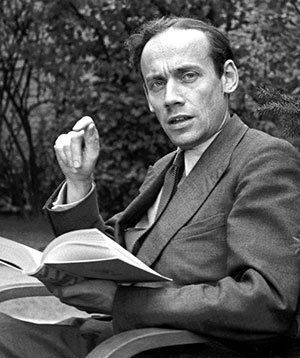
\includegraphics[scale=0.4]{img/emil-artin}
 \captionsetup{labelformat=empty}
 \caption{埃米尔$\cdot$阿廷 1898-1962}
 \label{fig:Emil-Artin}
\end{figure}
% https://milwaukeearmenians.com/2015/12/19/emil-artin/

1938年,德国数学家埃米尔$\cdot$阿廷对伽罗瓦的思想重新整理,他给出了伽罗瓦群的现代形式。对比阿廷的定义和伽罗瓦最初的定义,我们看出伽罗瓦的思想是如何一步一步走向清晰、简洁、成熟的。例如方程$x^2 - 2 = 0$有一对根$\pm \sqrt{2}$。显然用$-\sqrt{2}$去代替$\sqrt{2}$,方程仍然成立。除此之外,将等式$\sqrt{2}^2 + \sqrt{2} + 1 = 3 + \sqrt{2}$中的$\sqrt{2}$替换成$-\sqrt{2}$也是成立的。也就是说,这对根$\pm \sqrt{2}$,对于关系$\alpha^2 + \alpha + 1 = 3 + \alpha$是对称的。进一步说,对于任何仅仅对$\sqrt{2}$进行乘法和加法的表达式,这对根都可以进行互换。今天我们知道,描述对称的有力武器是群。这就是伽罗瓦当初引入置换群来研究方程的原因。阿廷看出了伽罗瓦群和域上的自同构的关系。考虑扩域$Q[\sqrt{2}]$,如果定义一个从$Q[\sqrt{2}]$到它自身的函数$f: Q[\sqrt{2}] \to Q[\sqrt{2}]$。它将$\sqrt{2}$的符号反转:
\[
f(a + b \sqrt{2}) = a - b \sqrt{2}
\]

则$f$就是一个域上的自同构。

\index{自同构}
\begin{definition}
\textbf{域的自同构}是一个可逆函数$f$,它将域映射到自身,并满足$f(x + y) = f(x) + f(y)$,$f(ax) = f(a) f(x)$,$f(1/x) = 1/f(x)$。
\end{definition}

我们可以验证,前面那个例子$f(a + b \sqrt{2}) = a - b \sqrt{2}$满足这三个条件。并且有趣的是反转正负号等效于置换方程的一对根$x_{1,2} = \pm \sqrt{2}$。域的自同构背后的思想是,我们可以重新调换域中的元素,而完全不影响域的结构。

\begin{definition}
$F$-自同构:进一步,如果$E$是$F$的扩域,并且在域$E$的自同构$f$的基础上还满足一条额外的性质:对$F$中的任何元素$x$都有$f(x) = x$,则称为$E$上的$F$-自同构。
\end{definition}

这样就非常精确地定义了根的对称性。$F$-自同构对$F$中的所有元素都原样保持不动,而仅仅调换扩域$E$中新元素。这个定义恰恰是伽罗瓦“如果已知则不变,如果不变则已知”的完美解释:元素是已知的,即$x \in F$,当且仅当在自同构下不变,即$f(x) = x$。对域中的元素进行调换恰好是置换的思想,置换后保持不变恰好是对称的概念。对于$Q[\sqrt{2}]$这个例子,只有两个$Q$-自同构:一个是恒等变换$e(x) = x$,另外一个就是$f(a + b\sqrt{2}) = a - b\sqrt{2}$。它们组成一个群$\{e, f\}$。这个群同构于循环群$C_2$和对称群$S_2$。它可以写成$\{f, f^2\}$,这是因为$f^2 = f \cdot f = e$。也可写成置换群的形式$\{(1), (1\ 2)\}$,其中(1)是保持两个根不变,(1 2)是对调两个根。

我们再给一个例子,方程$x^4 - 5x^2 + 6 = 0$的分裂域是$Q[\sqrt{2}, \sqrt{3}]$。我们有调换$\pm \sqrt{2}$的自同构$f$,也可以定义一个调换$\pm \sqrt{3}$的自同构$g(a + b\sqrt{3}) = a - b\sqrt{3}$。但是不存在能够调换$\sqrt{2}$和$\sqrt{3}$的$Q$-自同构。否则假设存在$h(\sqrt{2}) = \sqrt{3}$,则$h(\sqrt{2})^2 = h(\sqrt{2}^2) = h(2) = 2$。这是因为$f$保持乘法结构并且根据自同构的定义,对于有理数$x$有$h(x) = x$。但同时既然$h(\sqrt{2}) = \sqrt{3}$,则$h(\sqrt{2})^2 = \sqrt{3}^2 = 3$。于是推出$2 = 3$这样的矛盾。这说明并非$S_4$中的所有置换都反映了方程的对称性。这个方程的自同构有4个:$\{e, f, g, f \cdot g\}$,分别对应着恒等置换,对换$\pm \sqrt{2}$的$f$,对换$\pm \sqrt{3}$的$g$,和同时调换两对根的复合置换$f \cdot g$。它们构成一个群。

至此,我们已经把扩域和自同构联系了起来。把所有的自同构做成一个集合,这些自同构间的二元运算是复合变换,恒等变换是单位元,阿廷指出,这个群就是伽罗瓦群。

\index{伽罗瓦群}
\begin{definition}
\textbf{伽罗瓦群}的现代定义:对于$F$的扩域$E$,我们有一组$E$的$F$-自同构的集合$G$。对任意$G$中的两个$F$-自同构$f, g$,定义二元运算$(f \cdot g)(x) = f(g(x))$。我们称$G$为扩域$E/F$的伽罗瓦群。记为$Gal(E/F)$。
\end{definition}

\begin{mdframed}
通过根的对称性来研究方程是伽罗瓦思想中最优美的部分。现在我们终于可以利用自同构来精确定义对称了。所谓对称,就是组元的构形在其自同构变换群作用下所具有的不变性。
\end{mdframed}

\begin{Exercise}
\Question{试证明:对于有理数系数的任何多项式$p(x)$,若$E/Q$是扩域,$f$是$E$上的$Q$-自同构,则有$f(p(x)) = p(f(x))$。}
\Question{考虑复数,多项式$p(x) = x^4-1$的分裂域是什么?它的$Q$-自同构中有哪些变换?}
\Question{尝试写出二次方程$x^2 - bx + c = 0$的伽罗瓦群。}
\Question{证明,如果$p$是素数,则方程$x^p - 1$的伽罗瓦群是$p-1$阶的循环群$C_{p-1}$。}
\Question{若$\alpha$是方程$x^3 + x^2 - 4x + 1$的根,验证$2 − 2\alpha - \alpha^2$也是方程的根。方程在有理数域上的伽罗瓦群是什么?}
% from: https://math.stackexchange.com/questions/850818/find-the-galois-group-of-the-polynomial-when-a-root-is-given
% If $\alpha$ is a root of a polynomial $f(x) = x^3 + x^2 - 4x + 1$ then show that $2 − 2\alpha - \alpha^2$ is also a root of $f(x)$. Use this fact to compute the Galois group of the splitting field of $f(x) over $Q$.
% step 1: show f(2 − 2\alpha - \alpha^2) = 0
% step 2: let g(\alpha) = 2 − 2\alpha - \alpha^2, and
%             g^2(\alpha) = g(2 − 2\alpha - \alpha^2) \equiv \alpha^3 + \alpha - 3 (\bmod f(\alpha))
%             g^3(\alpha) = g(\alpha^3 + \alpha - 3) \equiv \alpha (\bmod f(\alpha)
% G = \{e, g, g^2\}
\end{Exercise}

\subsection{伽罗瓦基本定理}
\index{伽罗瓦基本定理}

现在我们进入了伽罗瓦理论的核心部分了。从方程系数所在的域$F$开始,我们可以进行一系列扩域一直到达分裂域$F \subset F_1 \subset F_2 ... \subset E$。对应的伽罗瓦群为$Gal(E/F)$。伽罗瓦发现,这个群的所有子群和这些中间域$F_1, F_2, ...$之间存在着反序的一一对应。

\begin{theorem}
\textbf{伽罗瓦基本定理}:令$E/F$为正规扩域,$G$是对应的伽罗瓦群。这个群的子群和中间域之间存在一一对应。若$F \subset L \subset E$,有$Gal(E/L) = H$,则$H$是$Gal(E/F)$的子群。
\end{theorem}

之所以说是反序,是因为,随着域的扩张,对应的群是缩小的。扩张的起点是域$F$,此时对应的群是完整的伽罗瓦群$G = Gal(E/F)$;扩张的终点是分裂域$E$,此时的群只有一个元素,就是恒等变换$\{e\}$。扩张的中间域$L$,对应的群是$H = Gal(E/L)$,它是子群,有$Gal(E/L) \subset Gal(E/F)$。并且如果$H$是正规子群,则它的商群$G/H = Gal(L/F)$。

例如方程$x^4 - 8x^2 + 15 = 0$,它可以表示成$(x^2 - 3)(x^2 - 5) = 0$。它的系数域是有理数域$Q$,方程的分裂域是$E = Q[\sqrt{3}, \sqrt{5}]$。它的伽罗瓦群$Gal(E/Q)$的阶是4,同构于一个4阶循环群。可以找到3个中间扩域分别是$Q[\sqrt{3}]$, $Q[\sqrt{5}]$和$Q[\sqrt{15}]$,这3个中间扩域对应的子群的阶都是2。而方程的伽罗瓦群,也就是4阶循环群只有一个2阶子群。除此之外,它不再有其它非平凡子群了。根据伽罗瓦基本定理,我们知道,除了那3个中间扩域之外,再也没有其它中间扩域了。换个角度看,分裂域上的任何元素都可以表示为$\alpha = a + b\sqrt{3} + c\sqrt{5} + d\sqrt{15}$,其中$a, b, c, d$是有理数;对于3个中间扩域上的任何元素,$b, c, d$中至少有两个为0。

\begin{figure}[htbp]
\centering
\begin{tikzpicture}[scale=0.8]
\draw (-3, 3) node (Q3-5) {$Q[\sqrt{3}, \sqrt{5}]$}
      (-5, 0) node (Q5) {$Q[\sqrt{5}]$}
      (-3, 0) node (Q15) {$Q[\sqrt{15}]$}
      (-1, 0) node (Q3) {$Q[\sqrt{3}]$}
      (-3, -3) node (Q) {$Q$};
\draw (3, 3) node (G1) {$\{1\}$}
      (1, 0) node (G3) {$\{1, f\}$}
      (3, 0) node (G15) {$\{1, (f \cdot g)\}$}
      (5, 0) node (G5) {$\{1, g\}$}
      (3, -3) node (G) {$\{1, f, g, (f \cdot g)\}$};
\draw[->] (Q3-5) edge node[midway, above] {伽罗瓦群} (G1)
      (G) edge node[midway, above] {对应到扩域} (Q)
      (Q3) edge node[midway] {扩域} (Q3-5)
      (Q15) edge (Q3-5)
      (Q5) edge (Q3-5)
      (Q) edge (Q3)
      (Q) edge (Q15)
      (Q) edge (Q5)
      (G1) edge node[midway] {子群} (G3)
      (G1) edge (G15)
      (G1) edge (G5)
      (G3) edge (G)
      (G15) edge (G)
      (G5) edge (G);
\end{tikzpicture}
\caption{伽罗瓦对应}
\label{fig:Galois-Correspondence}
\end{figure}

如图\ref{fig:Galois-Correspondence}所示,分裂域上的任意元可以写成如下形式:

\[
\begin{array}{rl}
\alpha &= (a + b\sqrt{3}) + (c + d\sqrt{3}) \sqrt {5} \\
       &= a + b\sqrt{3} + c\sqrt{5} + d\sqrt{15}
\end{array}
\]

其中$a, b, c, d$都是有理数。我们定义如下自同构:

变换$f$将$\sqrt{3}$反号:

\[
\begin{array}{rl}
f((a + b\sqrt{3}) + (c + d\sqrt{3}) \sqrt {5}) & = (a - b\sqrt{3}) + (c - d\sqrt{3})\sqrt{5} \\
 & = a - b\sqrt{3} + c\sqrt{5} - d\sqrt{15}
\end{array}
\]

变换$g$将$\sqrt{5}$反号

\[
\begin{array}{rl}
g((a + b\sqrt{3}) + (c + d\sqrt{3}) \sqrt {5}) & = (a + b\sqrt{3}) - (c + d\sqrt{3})\sqrt{5} \\
 & = a + b\sqrt{3} - c\sqrt{5} - d\sqrt{15}
\end{array}
\]

复合变换$f \cdot g$同时将$\sqrt{3}$和$\sqrt{5}$反号

\[
\begin{array}{rl}
(f \cdot g)((a + b\sqrt{3}) + (c + d\sqrt{3}) \sqrt {5} & = (a - b\sqrt{3}) - (c - d\sqrt{3})\sqrt{5} \\
 & = a - b\sqrt{3} - c\sqrt{5} + d\sqrt{15}
\end{array}
\]

\begin{figure}[htbp]
\centering
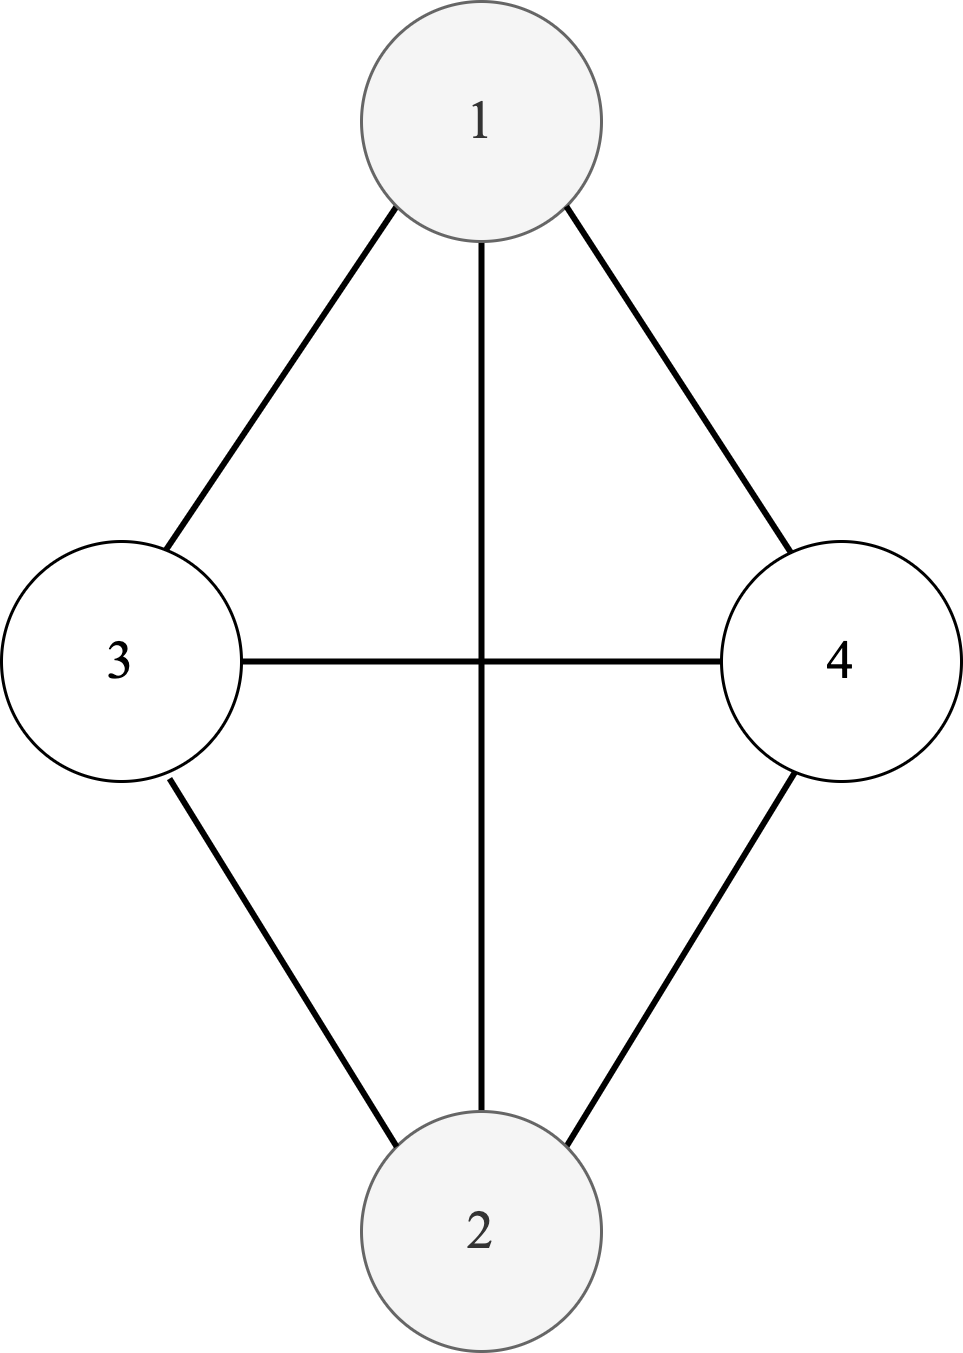
\includegraphics[scale=0.4]{img/K4}
\caption{克莱因群($K_4$)的对称性。左右翻转,上下翻转,或者同时上下左右翻转都是对称的。}
\label{fig:Klein-four-group}
\end{figure}

再加上恒等变换1,基本域$Q$上的伽罗瓦群一共有4个元素:$G = \{1, f, g, (f \cdot g)\}$。这个群同构于克莱因群$K_4$,而$K_4$相当于是两个循环群$C_2$的积。它共有5个子群,每个都对应着一个扩域:

\begin{enumerate}
\item 只含有单位元$\{1\}$的子群,对应于分裂域$Q[\sqrt{3}, \sqrt{5}]$;
\item $G$自身,对应于有理数域$Q$;
\item 二阶子群$\{1, f\}$,对应于扩域$Q[\sqrt{5}]$,$f$只反转$\sqrt{3}$而固定$\sqrt{5}$不变;
\item 二阶子群$\{1, g\}$,对应于扩域$Q[\sqrt{3}]$,$g$只反转$\sqrt{5}$而固定$\sqrt{3}$不变;
\item 二阶子群$\{1, (f \cdot g)\}$,对应于扩域$Q[\sqrt{15}]$,$(f \cdot g)$同时反转$\sqrt{5}$和$\sqrt{3}$,而固定$\sqrt{15}$不变。
\end{enumerate}

我们也可以把这个方程的伽罗瓦群写成置换群的形式:$\{(1), (1 2), (3 4), (1 2)(3 4)\}$。其中置换(1)表示保持4个根都不变;(1 2)表示交换$\pm \sqrt{3}$这两个根;(3 4)表示交换$\pm \sqrt{5}$这两个根;(1 2)(3 4)表示同时交换这两对根。通过伽罗瓦基本定理,我们已经成功地将方程在域上的问题,转换为对称群的问题了。接下来要做的就是最后一击,通过群揭示可解性的本质。

\subsection{可解性}

\begin{definition}
多项式方程根式可解,当且仅当它的根域$E$是基本域$F$的根式扩域。
\end{definition}

我们可以从基本域$F = Q$开始,不断通过根式扩域加入前一个域中某个元素的素数次方根或者本原单位根,最终可以到达方程的根域$E = F[\alpha_1, ..., \alpha_k]$。这样就可以形成了域的“根式塔”:

\[
F = F_0 \subseteq F_1 \subseteq F_2 \subseteq ... \subseteq F_k = E
\]

其中每个$F_i = F_{i-1}[\alpha_i]$,而$\alpha_i$是$F_{i-1}$中某个元素的素数次方根或本原单位根。通过伽罗瓦对应,根式扩域的结构就和群的结构联系起来了,和这一系列不断扩大的域塔对应的,是一系列缩小的子群塔:

\[
Gal(F_k/F_0) = G_0 \rhd G_1 \rhd ... \rhd G_k = Gal(F_k/F_k) = \{e\}
\]

其中,每一个群都是上一个的正规子群,每一步从$G_{i-1}$前进到它的子群$G_i$,都反应了向域$F$中扩张某个$\alpha_i$。伽罗瓦看出了根式扩域和伽罗瓦群缩小之间的规律。伽罗瓦每次向域中加入的是最小多项式$f_t(X)$的全部$p$个根,其中$p$为素数。正规扩域后对应的伽罗瓦群$H$将原来的群划分为$p$个陪集:
\[
G = \sigma_1H + \sigma_2H + ... \sigma_pH
\]
其中$H$为不变子群,而这些陪集组成的商群$G/H$的阶等于素数$p$。从练习\ref{ex:p-grp-abelian}的结论可知,素数阶群$p$一定是阿贝尔群(可交换的),因此根式扩域时,伽罗瓦群缩小后产生的商群是阿贝尔群。

\begin{definition}
\textbf{可解群}:$G$是一个有限群,如果存在一个$G$的子群列
\[
  G = G_0 \rhd G_1 \rhd ... \rhd G_k = \{e\}
\]
使得每个商群$G_i/G_{i+1}$都是阿贝尔群(可交换),则称$G$是一个可解群,上述群列为一个可解群列。
\end{definition}

从定义可以直接得出,可解群列中的任何子群都是可解群。另外任何阿贝尔群都有$G \rhd \{e\}$,所有阿贝尔群都是可解群。

伽罗瓦应用他的理论揭示出了多项式方程根式可解的答案:

\begin{theorem}
多项式方程根式可解,当且仅当它的伽罗瓦群是可接群。
\end{theorem}

对于一般3次方程,3个根的全部置换构成群$S_3$,它有一个正规子群$C_3$,$C_3$是单群,只有一个子群$\{e\}$。参考图\ref{fig:S3-Cayley},我们有群列:

\[
S_3 \rhd C_3 \rhd \{e\}
\]

对应商群的阶: $S_3/C_3 = 2, C_3/\{e\} = 3$都是素数,是可解群列。因此一般三次方程可解。

对于一般4次方程,4个根的全部置换构成群$S_4$,有24个元素。它有一个正规子群,是交错群$A_4$,有12个元素,如图\ref{fig:A4-Cayley}所示。接下来的正规子群是克莱因群$K_4$,有4个元素;而它又有正规子群$C_2$(同构于$S_2$),这是一个单群,只有一个子群$\{e\}$。我们有群列:

\begin{figure}[htbp]
 \centering
 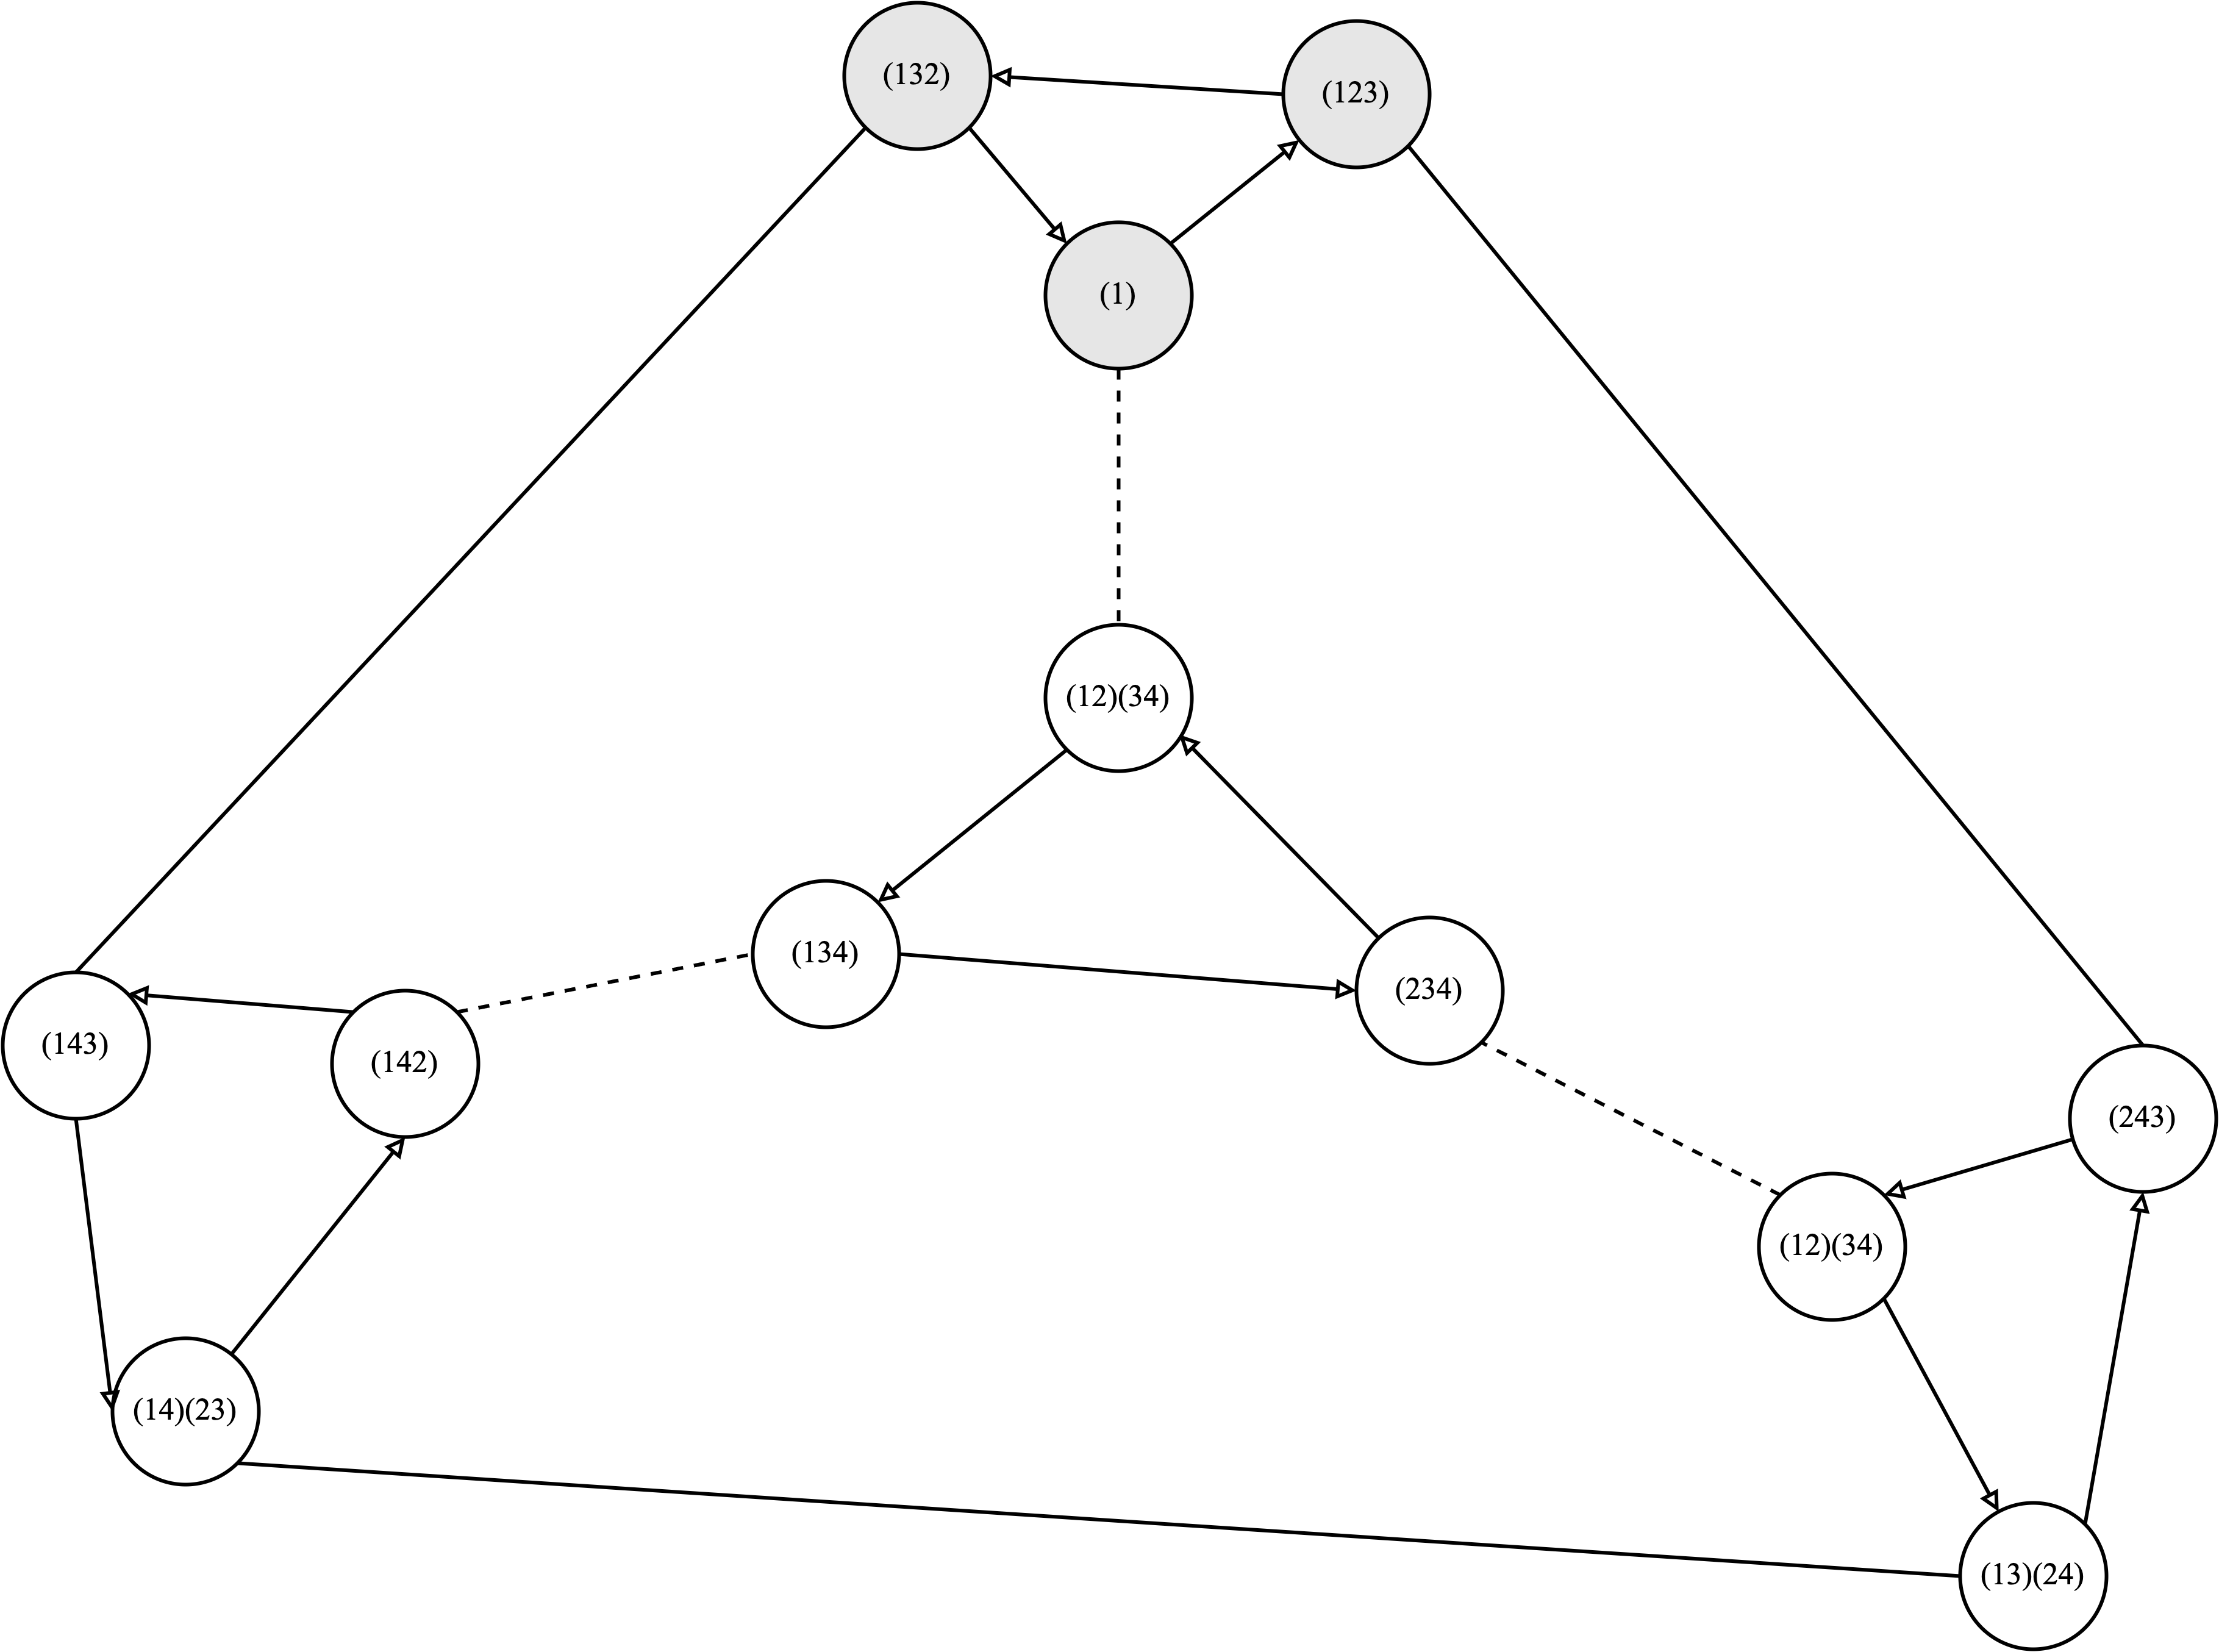
\includegraphics[scale=0.4]{img/A4-Cayley}
 \caption{交错群$A_4$的形状像一个三棱锥被截去了3个顶角}
 \label{fig:A4-Cayley}
\end{figure}
% http://weddslist.com/groups/cayley-31/index.html
% A graph illustrate K4 and A4: https://math.stackexchange.com/questions/651053/visualize-a-4-and-langle-x-z-rangle-isomorphic-to-the-klein-4-group

\[
S_4 \rhd A_4 \rhd K_4 \rhd C_2 \rhd \{e\}
\]

对应商群的阶分别是2、3、2、2,都是素数,是可接群列。因此一般4次方程可解。

从伽罗瓦理论可以直接推出阿贝尔——鲁菲尼定理:一般5次方程根式不可解。5个根的全部置换构成对称群$S_5$,有120个元素,它唯一的正规子群是交错群$A_5$,有60个元素,如图\ref{fig:A5-Cayley}所示。但是$A_5$是一个单群,它唯一的正规子群是$\{e\}$。我们有群列:

\[
S_5 \rhd A_5 \rhd \{e\}
\]

但是商群$A_5/\{e\}$同构于$A_5$,而$A_5$不是阿贝尔群。商群的阶是60,不是素数。因此它不是可解群。这样一般5次方程不是根式可解的。

\begin{figure}[htbp]
 \centering
 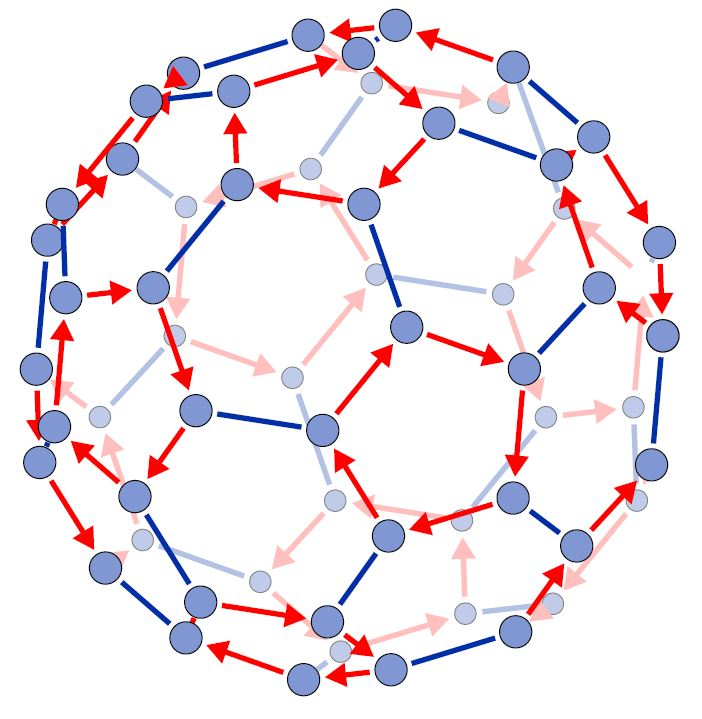
\includegraphics[scale=0.25]{img/A5-Cayley}
 \captionsetup{labelformat=empty}
 \caption{交错群$A_5$的形状像一个足球}
 \label{fig:A5-Cayley}
\end{figure}

我们还可以推出$n > 5$时,$S_n$也都不是可解群(见练习\ref{ex:3-cycle},用反证法,这会导致$\{e\}$包含3循环的矛盾)。应用伽罗瓦理论,一般5次以上的多项式方程也都不是根式可解的。

伽罗瓦正是通过对方程对称性的研究,发展出了伽罗瓦理论。它是抽象思想的明珠,是理性思维的强大工具。它可以解决很多问题,如证明正17边形可以用尺规作出,这是高斯年轻时发现的结论。伽罗瓦理论给出古希腊三大作图问题——圆化方、三分角、倍立方的否定答案,它们都无法用尺规作出。

\begin{Exercise}
\Question{考虑5次方程$x^5 - 1 = 0$,它是根式可解的。它的伽罗瓦群和对应的子群列是什么?}
\Question{证明:当$n \geq 5$时,设$S_n$的子群$G$含有所有的3循环,形如$(abc)$,$N$是$G$的一个正规子群,商群$G/N$是阿贝尔群。则$N$也含有所有的三循环。}
\label{ex:3-cycle}
\end{Exercise}

%% \section{扩展阅读}

%% 对于抽象代数的基本概念,张禾瑞先生的《近世代数基础》\cite{ZhangHeRui1978}是本入门的教材。这本书不到200页,提纲挈领地介绍了群、环、域的基本概念。阿姆斯特朗的《群与对称》\cite{Armstrong1988}同样也是小薄本,对于对称性的讲解是其特色。爱德华兹的《伽罗瓦理论》以历史的发展为主要脉络,还原了伽罗瓦理论是如何从牛顿、范德蒙德、拉格朗日的思想中逐步演进的。这本书基本沿用了伽罗瓦当初的的方法,并且还把伽罗瓦手稿的英文译文置于附录。埃米尔$\cdot$阿廷的《伽罗瓦理论》用现代方法重新整理了伽罗瓦理论,使用向量空间和域上的自同构进行改造,使得伽罗瓦理论具备了今天清晰、优雅的形式,是这个领域中的经典。韩雪涛的《好的数学》系列中有很多数学家的传记故事,生动有趣。

\section{附录}
伽罗瓦在他的论文中列出了一般4次方程伽罗瓦群缩小的群列。他当时还没有凯莱图这样的工具,于是用$abcd$代表方程的4个根,通过它们的置换表达了自己的思想。

\vspace{5mm}
\begin{center}

\begin{tabular}[t]{|c|}
\hline
$S_4$ \\
\hline
abcd \\
badc \\
cdab \\
dcba \\
acdb \\
cabd \\
dbac \\
bdca \\
adbc \\
dacb \\
bcad \\
cbda \\
bacd \\
abdc \\
dcab \\
cdba \\
cadb \\
acbd \\
bdac \\
dbca \\
dabc \\
adcb \\
cbad \\
bcda \\
\hline
\end{tabular}
\parbox[t]{3mm}{\vspace{2mm} $\rhd$}
\begin{tabular}[t]{|c|}
\hline
$A_4$ \\
\hline
abcd \\
badc \\
cdab \\
dcba \\
acdb \\
cabd \\
dbac \\
bdca \\
adbc \\
dacb \\
bcad \\
cbda \\
\hline
\\
\\
\\
\\
\\
\\
\\
\\
\\
\\
\\
\\
\hline
\end{tabular}
\parbox[t]{3mm}{\vspace{2mm} $\rhd$}
\begin{tabular}[t]{|c|}
\hline
$K_4$ \\
\hline
abcd \\
badc \\
cdab \\
dcba \\
\hline
\\
\\
\\
\\
\hline
\\
\\
\\
\\
\hline
\end{tabular}
\parbox[t]{3mm}{\vspace{2mm} $\rhd$}
\begin{tabular}[t]{|c|}
\hline
$C_2$ \\
\hline
abcd \\
badc \\
\hline
\\
\\
\hline
\end{tabular}
\parbox[t]{3mm}{\vspace{2mm} $\rhd$}
\begin{tabular}[t]{|c|}
\hline
$\{e\}$ \\
\hline
abcd \\
\hline
\\
\hline
\end{tabular}
\end{center}

\ifx\wholebook\relax \else
\begin{thebibliography}{99}

\bibitem{HanXueTao16}
韩雪涛 ``数学悖论与三次数学危机''. 人民邮电出版社. 2016, ISBN: 9787115430434

\bibitem{LiuXinyu2017}
刘新宇 ``算法新解'' 人民邮电出版社. 2017, ISBN: 9787115440358

\bibitem{HanXueTao2009}
韩雪涛 ``好的数学——“下金蛋”的数学问题''. 湖南科学技术出版社. 2009, ISBN: 9787535756725

\bibitem{HanXueTao2012}
韩雪涛 ``好的数学——方程的故事''. 湖南科学技术出版社. 2012, ISBN: 9787535770066

\bibitem{Wiki-Galois-theory}
Wikipedia ``伽罗瓦理论''. \url{https://en.wikipedia.org/wiki/Galois_theory}

\bibitem{Wiki-Galois}
Wikipedia ``埃瓦里斯特$\cdot$伽罗瓦''. \url{https://en.wikipedia.org/wiki/Évariste_Galois}

\bibitem{StepanovRose15}
[美] 亚历山大 A$\cdot$斯捷潘诺夫,丹尼尔 E$\cdot$罗斯著,爱飞翔译. ``数学与泛型编程:高效编程的奥秘''. 机械工业出版社. 2017, ISBN: 9787111576587

\bibitem{Wiki-Rubik-Cube-group}
Wikipedia ``魔方群''. \url{https://en.wikipedia.org/wiki/Rubik's_Cube_group}

\bibitem{ZhangHeRui1978}
张禾瑞 ``近世代数基础''. 高等教育出版社. 1978, ISBN: 9787040012224

\bibitem{Armstrong1988}
M.A. Armstrong ``群与对称(影印版)''. Springer. 1988. ISBN: 0387966757.

\bibitem{Wiki-Lagrange}
Wikipedia ``约瑟夫$\cdot$拉格朗日''. \url{https://en.wikipedia.org/wiki/Joseph-Louis_Lagrange}

\bibitem{Wiki-FLT-proof}
Wikipedia ``费马小定理的证明''. \url{https://en.wikipedia.org/wiki/Proofs_of_Fermat's_little_theorem}

\bibitem{Wiki-Euler}
Wikipedia ``莱昂哈德$\cdot$欧拉''. \url{https://en.wikipedia.org/wiki/Leonhard_Euler}

\bibitem{Wiki-Carmichael-number}
Wikipedia ``卡迈克尔数''. \url{https://en.wikipedia.org/wiki/Carmichael_number}

\bibitem{Algorithms-DPV}
Sanjoy Dsgupta, Christos Papadimitriou, Umesh Vazirani. 钱枫 邹恒明 注释. ``算法概论(注释版)''. 机械工业出版社. 2009年1月. ISBN: 9787111253617

\bibitem{Wiki-Miller-Rabin}
Wikipedia ``米勒——拉宾素数检验''. \url{https://en.wikipedia.org/wiki/Miller-Rabin_primality_test}

\bibitem{Wiki-Noether}
Wikipedia ``埃米$\cdot$诺特''. \url{https://en.wikipedia.org/wiki/Emmy_Noether}

\bibitem{ZhangPu2013}
章璞. ``伽罗瓦理论:天才的激情''. 高等教育出版社. 2013年5月. ISBN: 9787040372526

\bibitem{Stillwell1994}
John Stillwell. ``Galois Theory for Beginners''. The American Mathematical Monthly, Vol. 101, No. 1 (Jan., 1994), pp. 22-2

\bibitem{Goodman2011}
Dan Goodman. ``An Introduction to Galois Theory''. \url{https://nrich.maths.org/1422}

\bibitem{MArtin}
Michael Artin. ``代数(英文版,第二版)''. 机械工业出版社. 2011年12月. ISBN: 9787111367017

\bibitem{Weyl1952}
赫尔曼 $\cdot$ 外尔 著 冯承天、陆继宗 译. ``对称''. 北京大学出版社. 2018年7月. ISBN: 9787301291719

\end{thebibliography}

\expandafter\enddocument
%\end{document}

\fi
